\documentclass{scrreprt} % <= Druckversion: "scrbook" / Bildschirmversion: "scrreprt"
\usepackage[english,bibtex]{osm-thesis} % <= Sprache der Arbeit ("ngerman"/"english"), Biblatex-Backend ("bibtex"/"biber")

\usepackage{amssymb}
\usepackage{tabularx}
\usepackage{xspace}

% ABOUT
\newcommand{\hpitype}{Masterarbeit}
\newcommand{\hpiauthor}{Hendrik Tjabben}
\newcommand{\hpititle}{V 0.4}
\newcommand{\hpititleother}{TODO} % <= das Studienreferat verlangt einen deutschen UND englischen Titel
\newcommand{\hpisupervisor}{Prof.\,Dr.\,Andreas Polze, Robert Schmid, Lukas Pirl, Arne Boockmeyer}
\newcommand{\hpichair}{Professur für Betriebssysteme und Middleware}
\newcommand{\hpiexternalsupervisor}{Jakob Gärtner}
\newcommand{\hpiexternal}{Railergy}
\newcommand{\hpidate}{\today}


\newcommand{\etal}{\textit{et al.}\xspace}
\newcommand{\abr}{\gls*}
\newcommand{\abrpl}{\glspl*}

\usepackage[acronym]{glossaries}
\newacronym{ATO}{ATO}{Automatic Train Operation}
\newacronym{CPU}{CPU}{Central Processing Unit}
\newacronym{DCPS}{DCPS}{Data-Centric Publish-Subscribe}
\newacronym{DDS}{DDS}{Data Distribution Service}
\newacronym{ECC}{ECC}{Error Checking and Correction}
\newacronym{ERTMS}{ERTMS}{European Rail Traffic Management System}
\newacronym{ETCS}{ETCS}{European Train Control System}
\newacronym{FCR}{FCR}{Fault Containment Region}
\newacronym{FDI}{FDI}{failure detection and identification}
\newacronym{MA}{MA}{Movement Authority}
\newacronym{MOON}{MooN}{M-out-of-N}
\newacronym{OMG}{OMG}{Object Management Group}
\newacronym{OS}{OS}{Operating System}
\newacronym{PFD}{PFD}{probability to fail on demand}
\newacronym{QOS}{QoS}{Quality of Service}
\newacronym{SIL}{SIL}{Safety Integrity Level}
\newacronym{TMR}{TMR}{Tripple Modular Redundancy}


% DOCUMENT
\bibliography{bibliography}

\begin{document}

	% Einband
	\pagenumbering{alph}
	\ifisbook\begin{titlepage}
	\setlength{\evensidemargin}{0.5\evensidemargin+0.5\oddsidemargin}
	\setlength{\oddsidemargin}{\evensidemargin}

	\centering

	\raisebox{-0.5\height}{\includegraphics[width=5.5cm]{images/hpi_logo_black.pdf}}
	\hspace*{.2\textwidth}
	\raisebox{-0.5\height}{\includegraphics[width=4cm]{images/uni_logo_black.pdf}}
	
	\vspace*{4\baselineskip}
	{\usekomafont{subject}\hpitype}\par
	
	\vfill
	{\usekomafont{title}\hpititle\par}
	\vspace*{\baselineskip}
	{\usekomafont{subtitle}\hpititleother}\par
	
	\vfill
	{\textbf{\phantom{\iflanguage{ngerman}{von}{by}}} \\
	 \smallskip\usekomafont{author}\hpiauthor}\par
	
	\vfill
	\phantom{\begin{minipage}{\textwidth}
	{\textbf{\iflanguage{ngerman}{Betreuung}{Supervisors}}\\
	\usekomafont{publishers}\smallskip\hpisupervisor\\ \textit{\hpichair}\\ \smallskip\textbf{\normalfont\hpiexternalsupervisor}\\ \textit{\hpiexternal}}
	\end{minipage}}
	
	\vfill
	{\usekomafont{date}\iflanguage{ngerman}{Hasso-Plattner-Institut an der Universität Potsdam}{Hasso Plattner Institute at University of Potsdam}}\par
	\vspace*{\baselineskip}
	{\usekomafont{date}\hpidate}\par
	
\end{titlepage}\fi
	\ifisbook\cleardoubleemptypage\fi

	% (Haupt-)Titelseite, Abstract, ggf. Danksagung & Inhaltsverzeichnis
	\pagenumbering{roman}
	\begin{titlepage}
	\centering

	\raisebox{-0.5\height}{\includegraphics[width=5.5cm]{images/hpi_logo_srgb.pdf}}
	\hspace*{.2\textwidth}
	\raisebox{-0.5\height}{\includegraphics[width=4cm]{images/uni_logo_srgb.pdf}}

	\vspace*{4\baselineskip}
	{\usekomafont{subject}\hpitype}\par
	
	\vfill
	{\usekomafont{title}\hpititle\par}
	\vspace*{\baselineskip}
	{\usekomafont{subtitle}\hpititleother}\par
	
	\vfill
	{\textbf{\iflanguage{ngerman}{von}{by}}\\ 
		\smallskip\usekomafont{author}\hpiauthor}\par
	
	\vfill
	{\textbf{\iflanguage{ngerman}{Betreuung}{Supervisors}}\\ 
		\usekomafont{publishers}\smallskip\hpisupervisor\\ \textit{\hpichair}\\ \smallskip\textbf{\normalfont\hpiexternalsupervisor}\\ \textit{\hpiexternal}}
	
	\vfill
	{\usekomafont{date}\iflanguage{ngerman}{Hasso-Plattner-Institut an der Universität Potsdam}{Hasso Plattner Institute at University of Potsdam}}\par
	\vspace*{\baselineskip}
	{\usekomafont{date}\hpidate}\par

	\setcounter{page}{1}

\end{titlepage}


	% \ifisbook\cleardoubleemptypage\fi% => Wenn die Arbeit auf Deutsch verfasst wurde, verlangt das Studienreferat KEINEN englischen Abstract

% % englischer Abstract
\null\vfil
%\begin{otherlanguage}{english}
\begin{center}\textsf{\textbf{\abstractname}}\end{center}
%
\noindent \glsentryfull{ETCS} on-board units are safety-critical systems whose reliability plays a vital role in the integrity of railway operation.
While redundancy is a typical method for increasing fault tolerance, reliability, and safety, it also adds a communication and computation overhead.
Further, the development and maintenance of highly safety-critical applications are resource-intensive.
This thesis provides background and implementation of a redundant and fault-tolerant ETCS on-board system using real-time \glsentryfull{DCPS} machine-to-machine communication and consensus-based voting.
Besides behavioral concepts, such as a leader election and decision-making algorithm, the work exposes global system state and system recovery mechanisms in distributed systems.
The implementation's functionality, safety, and reliability are evaluated based on a subset of ETCS in a simulated environment.
The results confirm DCPS concepts applicable for solving the communication and computation overhead of distributed and redundant computation in a real-time and safety-critical environment.
Furthermore, the findings also apply to an architecture of general-purpose Programmable Logic Controllers (PLCs).
Thereby, this work facilitates the development of safe and more cost-efficient on-board systems for future ETCS applications.

%\end{otherlanguage}
\vfil\null

% => Wenn die Arbeit auf Englisch verfasst wurde, verlangt das Studienreferat einen englischen UND deutschen Abstract (der dt. Abstract kann dann ggf. auch ans Ende der Arbeit)

% deutsche Zusammenfassung
\null\vfil
\begin{otherlanguage}{ngerman}
\begin{center}\textsf{\textbf{\abstractname}}\end{center}

\noindent 

Die Fahrzeugsysteme des Europäischen Zugbeeinflussungssystems (ETCS) sind sicherheitskritische Systeme, deren Zuverlässigkeit eine entscheidende Rolle bei der Betriebssicherheit der Bahn spielt.
Um die Fehlertoleranz, die Zuverlässigkeit und die Sicherheit von Systemen zu erhöhen, werden üblicherweise redundante Informationen und Berechnungen verwendet.
Diese führen allerdings auch zu einem erhöhten Kommunikations- und Bearbeitungsaufwand.
Darüber hinaus sind Entwicklung und Instandhaltung von sicherheitskritischen Anwendungen ressourcenintensiv.
In dieser Arbeit werden Grundlagen, Funktionsweisen und die Implementierung eines verteilten, redundanten und fehlertoleranten ETCS-Fahrzeugsystems vorgestellt.
Die systeminterne Kommunikation basiert auf einer echtzeitfähigen Zwischenanwendung, die dem datenzentralen Publish-Subscribe (DCPS) Muster folgt.
Weiterhin werden redundante Zwischenergebnisse über ein konsensbasiertes Abstimmungsverfahren dedupliziert.
Neben Verhaltenskonzepten, wie der Wahl eines Systemanführers und einem Entscheidungsfindungsalgorithmus, stellt diese Arbeit Möglichkeiten für einen globalen Systemzustand und zur Erholung von Fehlern in verteilten Systemen vor.
Die Evaluation von Funktionalität, Sicherheit und Zuverlässigkeit der Implementierung erfolgt in einer simulierten Umgebung, basierend auf einer Teilmenge von ETCS.
Die Ergebnisse bestätigen die Anwendbarkeit von DCPS-Konzepten zur Lösung des Kommunikations- und Rechenaufwandes verteilter und redundanter Systeme in echtzeit- und sicherheitskritischen Umgebungen.
Darüber hinaus zeigt sich, dass die Erkenntnisse auch für eine Architektur von universell einsetzbaren Speicherprogrammierbaren Steuerungen (SPS) gelten. 
Dadurch erleichtert diese Arbeit die zukünftige Entwicklung von sicheren und kostengünstigen ETCS-Fahrzeugsystemen.

\end{otherlanguage}
\vfil\null



	%\ifisbook\cleardoubleemptypage\fi\vspace*{\fill}
\begin{center}\textsf{\textbf{Acknowledgment}}\end{center}

\noindent Throughout the writing of my thesis I have received great support and assistance.
\\

\noindent First of all, I would like to thank my supervisor, Prof. Andreas Polze, whose expertise and systematic methodology was inevitably for this work's structure and success.
\\

\noindent I would further like to acknowledge my tutors Robert Schmid, Lukas Pirl, and Arne Boockmeyer, who supported me with their valuable advice.
Besides all the tools I needed, you gave me indispensable and regular feedback to choose the right direction and successfully complete my thesis.
\\

\noindent I would also like to thank Jakob Gärtner for his dedication, support, and insights.
Jakob, you not only provided the hardware for the project but also were decisive in formulating the research question.
Without you, this work would not have been possible.
\\

\noindent In addition, I would like to thank my family, my friends, and my partner.
You were always there for me during a time, where social contacts must be limited to a minimum.
Thank you for every conversation and any welcome distraction. 


\vspace*{\fill}
	\tableofcontents
	\cleardoublepage

	% Textteil
	\pagenumbering{arabic}
    \chapter{Introduction}

%https://www.myperfectwords.com/blog/thesis-writing/writing-a-thesis-introduction

% Attention grabbing hook statement
Railway operation is undergoing rapid changes.
%
% General introduction to topic through general statements
As digitalization progresses, a trend towards the \abr{IOT} is developing and devices such as vehicles and machines become interconnected~\cite{RailwayDigitalization}.
With the increasing traffic and the importance of the railway in the transportation of persons and goods alike, digitization offers a way to deal with growing complexity.

On the one hand, improvements in computation and communication technologies, as well as in railway applications, laid the foundation for building safe and reliable systems.
Studies have shown that 41\% of all railway accidents were caused by human failures~\cite{StudyRailwayAccidents}.
At the same time, \abr{SIL} 4 certified \abr{ATO} systems with a small \abr{PFD}~\cite{SallekSIL} are possible.
Further, the standardization of signaling and control components in the \abr{ETCS} facilitated train operation across borders and increased the significance of \abr{ATO} systems~\cite{YIN2017RNDofATO}.

On the other hand, the automation of railway operations comes with higher development and acquisition costs, as well as ethical issues.
System designers must specify the system's reaction under specific conditions and balance the safety of humans, such as passengers and road users, and of resources, such as costs and time~\cite{EthicsInSafety}.

Hence, with the railway being a safety-critical system, any component applied in the \abr{ETCS} context must comply with strict certification requirements to assure its safety and reliability.
Compliance with system requirements is ensured during an approval process.
The thereby applied verification, validation, and certification steps are time- and cost-intensive, which adds to the already high development costs.
Moreover, the approval process needs to be repeated every time the system gets updated.
Increasing costs for \abr{ETCS} systems could lead to a situation where it is not profitable to equip certain regions, connections, or train models with \abr{ETCS}.
\\

Distributed computation is a way to reduce the costs of repeated approval processes and increase scalability.
Therefore, autonomous computing elements - that each performs a subset of the system's requirements - are interconnected~\cite{DistributedSafety2020}.
However, distributed systems also introduce new challenges such as coping with the communication overhead and dealing with node-, network-, and computation faults.

A fundamental technique for coping with faults in a computing system is redundancy~\cite{TanenbaumSteen07}.
In redundant computation, safety-critical calculations are performed in parallel in a distributed manner and combined afterwards.
Generally speaking, redundancy entails additional resources that are not required for a system's functional operation but add specific characteristics such as fault detection and fault tolerance~\cite{BarryFaultToleranceAnalysis}.
Various well-established redundancy patterns have been proven in practice, including hardware-, software-, information-, and time redundancy.
In contrast to non-redundant systems, redundancy allows building safe systems out of less safe and cheaper parts.
\\

For handling communication in distributed systems, different concepts, standards, and frameworks exist.
One of them is \abr{DDS}, a \abr{DCPS} standard for machine-to-machine communication that is specified by the \abr{OMG}~\cite{omgDDSspec}.
\abr{DDS} is designed for facilitating safe and real-time communication among distributed and autonomous execution units and is therefore applicable for building safety-critical systems~\cite{DistributedSafety2020}.
The standard, which is intended to be implemented as a middleware, allows the specification of \abr{QOS} to define the service's behavior in a declarative way.
Through the \abrpl{QOS}, the communication can be defined to be reliable and real-time.

However, \abr{DDS} has been designed to be a generic standard for distributed application communication and integration and therefore provides a wide variety of features~\cite{omgDDSspec}.
Hence, every feature from the applied middleware implementation needs to be approved when applied in a safety-critical application.
\\

In this thesis, it is investigated whether the \abr{DDS} standard is applicable for building redundant, distributed, real-time, and safety-critical systems in the \abr{ETCS} domain.
One of the main requirements is that the application should run on general-purpose \abrpl{PLC} with limited resources without violating safety and reliability requirements.
This work makes the following \textit{contributions}:

\begin{enumerate}
\item An analysis and comparison of different established redundancy concepts based on their reliability and implementability with \abr{DDS}.
\item Elaboration and implementation of a consensus-based redundant architecture based on a fault model of an \abr{ETCS} subset.
\item A proof-of-concept evaluation of the implementation towards functionality, safety, and implementability with \abr{DDS}.
\item A sufficient \abr{DDS} subset for building a safety-critical and real-time distributed system.
\end{enumerate}

\paragraph{Structure}
First, an overview of popular redundancy patterns and characteristics for building safe and reliable systems, as well as about \abr{ETCS} and \abr{DDS}, is given in~\autoref{chptr:concepts}.
Afterward, mathematical concepts for evaluating the safety and reliability of these systems are pointed out.
A selection of related work that uses \gls{DDS} in safety-critical applications is presented and set in relation to this work at the end of chapter 2.
\\

In~\autoref{chptr:redundantSystemsCompare}, key building blocks for designing distributed systems with the \abr{DDS} standard are described.
The redundancy concepts and patterns previously presented are opposed and evaluated based on the characteristics from chapter 2.
Further, each pattern's exemplary concepts and architectures are described and assessed based on their safety and realizability with \abr{DDS} concepts.
Therefore, not only voting-based concepts but also a way of building consensus-driven redundant systems are described and analyzed.
A combination of a consensus- and voting-based approach is identified as the most suitable concept for satisfying the desired system's requirements.
\\

In~\autoref{cpt:Implementation}, an exemplary implementation is presented that follows the concepts of \texttt{Raft}~\cite{RaftConsensusPaper}.
Thereby, the significance of a safe consensus- and voting-based redundant system, which utilizes \abr{DDS} for communication, is shown.
The system comprises of four homogeneous and interconnected \textit{Revolution Pi} from Kunbus~\cite{Kunbus} and utilizes \textit{OpenSplice DDS} from ADLINK~\cite{VortexOpenSplice} as a \abr{DDS} framework.
A \textit{Revolution Pi} is a robust \abr{PLC} that build upon a \textit{Raspberry Pi} and features a real-time capable \abr{OS}.
The \textit{OpenSplice DDS} framework's applicability for safety-critical railway applications has been proven in practice~\cite{SchmidtMissionCriticalChallenges}.
\\

Afterward, the implemented system's safety and functional correctness are proven based on a simulated \abr{ETCS} scenario in~\autoref{cpt:evaluation}.
In addition, the system's time performances and hardware resource utilization is examined.
Results show the system runs the simulated scenarios successfully and all requirements are met, even when an entire component fails.
Finally, the applied \abr{DDS} subset is listed and justified.


%TODO Mention results and main realization


     \chapter{Background and Related Work}
\label{chptr:concepts}

All systems that are designed based on the \abr{ETCS} specification must be safety-critical~\cite{OnBoardUnitSafetyTesting}. 
Introducing redundancy to safety-critical systems is a popular approach to ensure that faults inside the system do not lead to failures that effect the system's environment.
A system that is able to continue its intended work even in the presence of faults is said to be fault-tolerant~\cite{BarryFaultToleranceAnalysis}.
Redundancy can be achieved in multiple ways, some of which being adding additional resources (hardware redundancy), adding additional information or messages (information redundancy), or performing the same operation multiple times (time redundancy).
Although being one of the most often used redundancy techniques, the addition of hardware components, called replicas for redundant computation, leads to multiple results which need to be consolidated to a final system result.
Thus, the replicas need to communicate with each other and synchronize their results in order to act like a single unit in their environment.
A promising approach to cope with the communication overhead is \gls*{DDS}, a \gls*{DCPS} system, since it allows reliable and real-time communication~\cite{omgDDSspec}.
However, while hardware redundancy enhances a system's fault-tolerance, it also increases its costs and complexity.
\\

In the first section of this chapter, an introduction to \abr{ETCS} and its three levels is provided.
Afterwards, an overview about the \abr{DDS} standard and its concepts is exposed.
In the third section, terms, criteria, and concepts for evaluating the safety and reliability of redundant systems are described.
Then, different redundancy concepts are explained and weighted against each other with regards to reliability, safety, and performance.
Finally, standards for building and designing safe and fault-tolerant systems are given and related works, that successfully applied \gls*{DCPS}-middleware in the railway context, are shown.

\section{\glsentryfull{ETCS}}
In order to facilitate interoperability between national railway systems throughout Europe, the signaling and speed control system has been standardized by the European Union under the term of \abr{ERTMS}.
\abr{ETCS} defines the signaling and train control component of \abr{ERTMS}~\cite{ETCS26}.
As such, \abr{ETCS} defines concepts for monitoring a train's speed, calculating the permissible speed restrictions, and coordinating the collaboration between track-side components, such as \abr{ETCS} euro-balises and on-board systems.
Any train requires a \abr{MA} to be allowed to drive from one location to another.
Besides encoding a train's permission to move, a \abr{MA} also encodes information about the track's conditions such as gradient proviles and speed limitation.
Any \abr{MA} is supplied by an external entity, called \abr{RBC}, via track-side components or via radio frequencies
A system that is located on the operating train - called on-board unit - monitors compliance with the current \abr{MA}.
The track-side components, as well as the on-board unit, are standardized according to three different \abr{ETCS} levels.

\paragraph{\abr{ETCS} level one}
\abr{ETCS} level one has been designed to build upon existing signaling systems.
\abrpl{MA} as well as route data and the maximum allowed speed are transmitted through fix positioned euro-balises.
Parallel to that, a breaking curve and the train's position are permanently calculated and compared to the \abr{MA}'s limitations by an on-board unit.

\paragraph{\abr{ETCS} level two}
For \abr{ETCS} level two, signaling and \abr{MA} data is transmitted via mobile communication channels from the \abr{RBC} and displayed to the driver.
The \abr{RBC} is a central unit that constantly collects and supervises train movements and track information.
Although each train observes its own position, it can come to inaccuracies, for example due to a faulty sensor calibration.
Hence, a train operating under \abr{ETCS} level two does not know its exact position but can only locate itself within a certain range.
This range is called \textit{confidence interval} and consists of an upper and lower limit of an area.
The train's actual position in located within this area.
In order for the on-board unit to determine a train's exact position, track-side balises are used.
Before the train starts its journey, the positions of the balises that it will encounter on its journey are provided during linking phase.
Thus, when a train crosses a linked balise and receives the balise telegram, the on-board unit can reset the train's position to the balises position.

\paragraph{\abr{ETCS} level three}
Finally, in \abr{ETCS} level three, any track-side component is abolished and the entire communication takes place via radio signals.
This \abr{ETCS} level is not fully standardized yet.

\section{\glsentryfull{DDS}}

\begin{figure}[!hb]
	\centering
	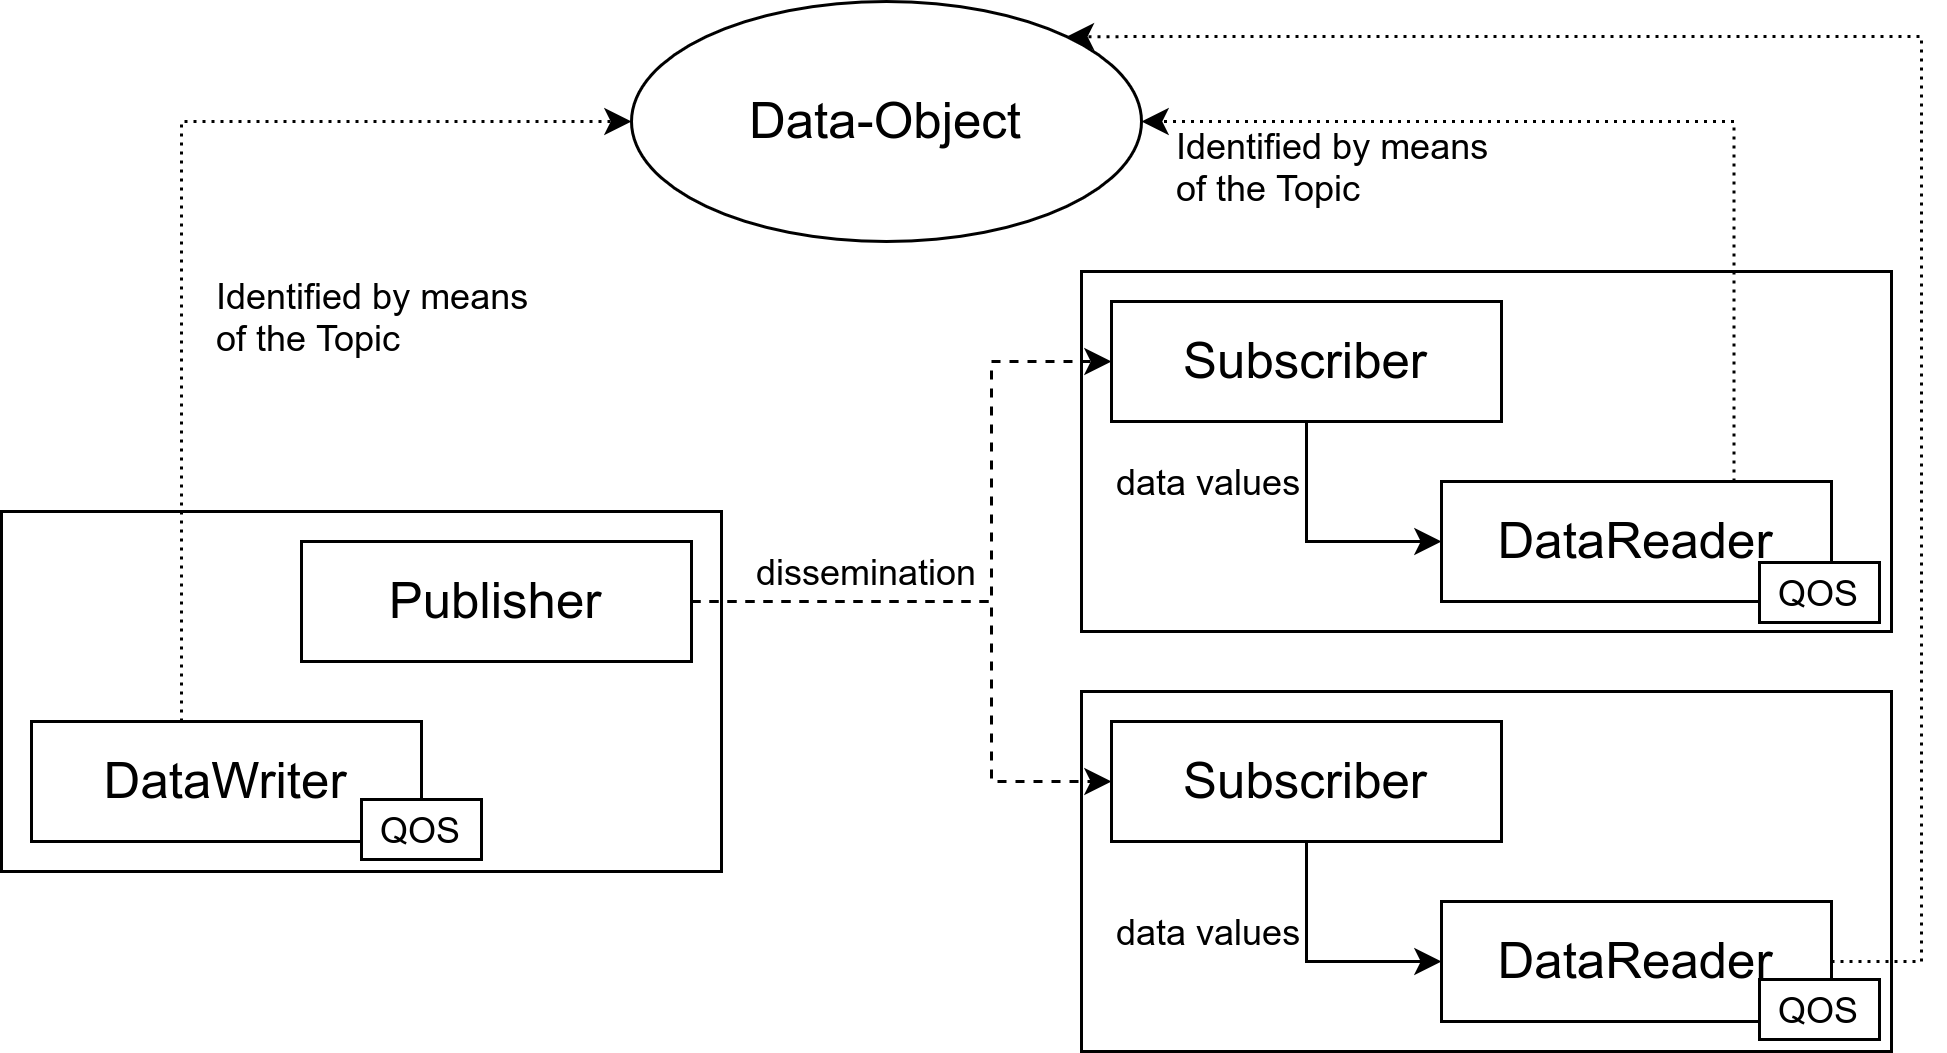
\includegraphics[width=0.75\linewidth]{images/DDSStructure}
	\caption{The \glsentryfull{DDS} is a data-centric communication model and follows the publish/subscribe pattern. The publishing and subscribing attendees do not communicate directly with each other, but make use of topics to read and write data objects.}
	\label{fig:DDSStructure}
\end{figure}

\Gls*{DDS} is a \gls*{DCPS} model for machine-to-machine communication, that is specified by the \gls*{OMG}~\cite{omgDDSspec}.
It is stated that the model should, for practical use, be implemented as a middleware in order to interface with the underlying \gls*{OS}.
The model follows the concept of a global data space and facilitates data exchange among entities based on type and content.
Central entities are \texttt{Publishers} and \texttt{Subscribers}, while data exchange is based on \texttt{Topics}.
A \texttt{Publisher} is used for sending data of different types.
In order to send specifically typed data, a \texttt{DataWriter} object is used which acts as a typed interface to a \texttt{Publisher}.
On the other side, a \texttt{Subscriber} is used to receive data and to make it accessible to the receiving application.
The equivalent of the \texttt{DataWriter} for the \texttt{Subscriber} is the \texttt{DataReader} object.
A \texttt{Topic} acts as the connecting element between publishing entities on the one side and subscribing entities on the other.
Any forecasting of when and how data is published to a \texttt{Topic} or received by a \texttt{Subscriber} is made possible through so called \glspl*{QOS} policies.
This concept is illustrated in~\autoref{fig:DDSStructure}, which is based on the official \gls*{DDS} specification~\cite{omgDDSspec} and shows the information flow from the publishing to the subscribing side.

An application can either rely on the middleware to asynchronously notify it about the presence of new data through so called \texttt{Listeners}, or actively wait for new data by utilizing \texttt{WaitSets}.
A \texttt{WaitSet} can be attached with different \texttt{Conditions}, for example \texttt{ReadConditions}, and allows the application to wait until either one or more of the attached conditions are satisfied, or until the waiting times out.
Examples for conditions are \texttt{ReadCondition} and \texttt{QueryCondition}.
The \texttt{ReadCondition} object allows to name specific data samples and is met when the specified type of data is present in a \texttt{DataReader}.
A \texttt{QueryCondition} is a specified \texttt{ReadCondition} that further provides capabilities of filtering the data that is read through a \texttt{DataReader}.
\\

The usefulness of \gls*{DDS} for containerization technologies in automotive architectures has been studied by Kugele \etal~\cite{KugeleDataCentricForAuto}.
Although their findings are based on containerization technologies and are therefore not resilient for this work, Kugele \etal showed that the applicability of \gls*{DDS} with regards to safety, certification and security depends on the actual implementation's characteristics.
Therefore, Vortex OpenSplice DDS is used throughout this thesis, which is being developed and maintained by ADLINK.

The applicability of the \gls*{DDS}-standard and of Vortex OpenSplice \gls*{DDS} for safety-critical railway applications has been demonstrated by Schmidt and van't Hag~\cite{SchmidtMissionCriticalChallenges}.
Their findings show, that OpenSplice \gls*{DDS}'s \gls*{QOS} policies allow predictable time and locality characteristics for data distribution.
Further, their work provides an overview about Vortex OpenSplice's \gls*{QOS} policies and features to ensure reliability, availability, data-delivery, and resource usage.

\section{Techniques for Safety and Reliability Evaluation}
\label{sec:techniquesSafetyReliability}
In order to profoundly express and analyze redundancy techniques towards their safety, reliability and fault-tolerance, it needs to be defined what these characteristics mean.
\\

Reliability is, by IEEE 610.12-1990, defined as the ability of a system or component to perform its required function under stated conditions for a specified period of time~\cite{ieee610.12}.
A circumstance where a system deviates from its requirement is called a system failure.
A failure is preceded by a fault, which describes a static defect of a system~\cite{AmmannOffutt2016}.
When a fault becomes active, it manifests itself as an error, which marks an incorrect internal system state.
An failure occurs as soon as the error affects the system's environment.

\begin{definition}
A failure of a system or a system component is a state where its actual behavior deviates from the its specified behavior.
\end{definition}

The definition of reliability used in this work is the following:

\begin{definition}
\label{def:reliability}
A system's reliability is a function of time that expresses the probability for the system to operate as specified at a time $t_1$, given that it was operating as specified at time $t | t \leq t_1$.
\end{definition}

In other words, reliability is a system's ability to not have any failure for a specific period of time.

A system's safety is associated with its reliability, since it constitutes an extension of reliability~\cite{AvizienisDependability2001}.
In general, safety defines the absence of catastrophic failures on a system's environment.
When the presence of non-catastrophic failures can be reliably detected and a safe state can be taken in case of failures, safety can be treated as reliability concerning catastrophic failures.
In other words, safety can be expressed as a system's probability to not experience any fault that would lead to a catastrophic failure in a specific time span.

Based on these definitions, it can be conducted that a system's safety and reliability can only be finally assessed when the system's environment, the reliability of the system's components and the operations performed by the system are known.
In addition, the system's architecture and structure need to be acquainted.
Finally, in order to specifically evaluate a system's safety, possible faults and their consequences need to be known.
In order to be able to evaluate and compare different architectural pattern towards their safety characteristics, independently of the subsequently conducted operations, the definition of \texttt{intrinsic safety}, made by~\cite{BoulangerStandards}, is used in this work.

\begin{definition}
A system is said to be intrinsically safe if one can be certain that any failure of one or more components of that system will only result in its becoming more permissive.
In the railway context, a complete stoppage is generally the safest state.
\label{def:intrinsic_safety}
\end{definition}

This definition requires that measures are taken to assure the system's safety even in the presence of failures.
A system that provides the functionality to behave as specified even in the case of faults is said to be fault tolerant~\cite{AvizienisDependability2001}.
Fault tolerance is generally obtained through error detection, which allows the system to determine the presence of errors and enables it to mitigate resulting failures.
In the course of this thesis, the following definition is used for safety:

\begin{definition}
A system is said to be safe when the fault of the system or any of its components does not lead to a catastrophic failure.
\label{def:safety}
\end{definition}

Thus, in order to be considered secure, a distributed system must tolerate possible faults that could occur in distributed systems.
Flaviu Cristian has established the following five fault classes for distributed distributed systems~\cite{CristianFaultModel}:

\begin{enumerate}
\item \textbf{F1:} One or multiple components in the system crash (\textbf{crash fault}).
\item \textbf{F2:} One or multiple components fail to respond to an incoming request (\textbf{omission fault}).
\item \textbf{F3:} One or multiple components fail to produce an output within a certain time span (\textbf{timing fault}).
\item \textbf{F4:} One or multiple components produce a wrong result (\textbf{computation fault}).
\item \textbf{F5:} One or multiple components produce arbitrary responses at arbitrary times (\textbf{byzantine fault}).
\end{enumerate}

It applies, that all fault classes \textbf{Fx} are included in \textbf{Fy}, given that $y \geq x$.
In the course of this thesis, the fault classes \textbf{F1} to \textbf{F4} are analyzed and byzantine faults are not covered.
\\

A required condition for a system to be safe is that the system is reliable.
One method of analyzing a system's reliability is through mathematical functions of time, for example the \texttt{exponential failure law}~\cite{GeffroyMotetDependableComputing}.
It describes a component's reliability as an exponential function on time.
\begin{equation}
R(t) = e^{-\lambda t}.
\label{eq:expFailureLaw}
\end{equation}
The parameter $\lambda$ is called the failure rate and encodes the probability of failures occurring in a certain time span, typically in an hour.
For the exponential failure law it is, mathematically, assumed that the components fail independently.
This might not always be the case in practice, as common core or power outage failures can affect multiple components at once.
However, the probability of failures affecting multiple components at once can be reduced by various techniques, such as using independent power supplies or diverse redundancy, the latter of which being discussed below.
\\

Among various theoretical techniques for evaluating a system's safety, Markov chains are one of the most commonly used~\cite{BarryFaultToleranceAnalysis}.
Markov chains are a stochastic process that models the alterations of a system's state and probabilities for the system to transition into a specific state given that it was in a certain state~\cite{KemenyMarkovChains}.
Thereby, the next state only depends on the current state and is independent from all previous system modifications.

For a safety analysis, each state models the system in one out of three conditions:
\begin{enumerate}
\item The system functions without having an error.
\item The system detects and successfully mitigates an error without leading to a failure
\item The system either not detects an error or does not recover from it, leading to a failure
\end{enumerate}

For the state transition probabilities, the exponential failure law~\autoref{eq:expFailureLaw}, with a constant failure rate $\lambda$, holds.

\begin{figure}[!hb]
	\centering
	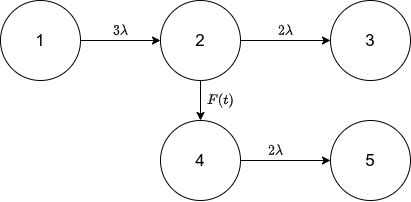
\includegraphics[width=0.75\linewidth]{images/TriplexSystemNASA}
	\caption{A reliability model for \glsentryfull{TMR} using Markov chains. In state (1), three replicas are operating redundantly. Each state transition describes the failure of a replica together with the corresponding probability.}
	\label{fig:NASATMR}
\end{figure}

An example Markov chain for a system using three replicas is proposed by NASA and depicted in~\autoref{fig:NASATMR}~\cite{NASAMarkovChains}.
At state (1), assuming that the system is homogeneous redundant, the probability that one of the replicas fails is $3\lambda$.
In state (2), the system applies failure detection and mitigation procedures and has a chance of $F(t)$ for successful reconfiguration, which allows the system to continue its work.
However, there is still a change of $2\lambda$ that another component fails before the system detects and mitigate the first failure, which would lead to a system fault and render the entire system unsafe.
In state (4), there is again a $2\lambda$ change for one of the remaining components to fail, which would lead to a failure of the entire system.

As experiments have shown, a system's recovery time is not necessarily exponential~\cite{TheoryAndPracticeReliableSystem}.
Thus, it is expressed by $F(t)$ which is the probability that the system recovers within a time-span less than $t$.
In a diverse redundant system, each component failure is represented with an individual state.

\section{Redundancy Patterns}
\label{sec:redundancyPatterns}
Redundancy is a typically applied technique for handling and masking errors in a system and thereby enhancing a system's reliability~\cite{TanenbaumSteen07}.
Error masking is the concept of detecting and mitigating errors, so that they do not become failures and effect the system's environment.
For redundancy, additional resources or information are added to a system, that would not be required when errors where impossible to happen.
Barry Johnson defines redundancy in the following way~\cite{BarryFaultToleranceAnalysis}:
\begin{definition}
The concept of redundancy implies the addition of information, resources, or time beyond what is needed for normal system operation.
Redundancy can take one of several forms, including hardware, software, information, and time redundancy.
\end{definition}

Each form of redundancy has its unique characteristics and patterns, which are presented in the following.

\subsection{Hardware Redundancy}
In hardware redundancy, additional replications of physical components are added to the system.
This typically increases the system's reliability by masking internal failures, but also increases the system's cost.
In general, a system's safety can be further improved when using components that are based on different internal components.
Using different components in redundancy patterns is called diverse redundancy, while replicating the same components is called homogeneous redundancy~\cite{HomogeneousRedundancyOuzineb}.
Using diverse redundancy has the benefit that it reduced the effect that common core errors have on a system's or component's safety.

Johnson subdivides hardware redundancy into two parts, namely passive and active redundancy.
In passive hardware redundancy, a voter or consensus algorithm is used to reduce a number of redundant outputs to a single output, in order to prevent individual internal failures from propagating out of the system.
In active hardware redundancy, the system tries to detect and repair any internal failure, for example by replacing the faulty component.
While \gls*{MOON} systems are a typical example of passive hardware redundancy, standby redundancy is often used as an example of active hardware redundancy.

A voter can be realized in both software and hardware.
The benefits of software voters are that they typically cost less and are easier to develop, because no special hardware is required.
However, software voters tend to operate slower.
The benefit of hardware voters is, that they can operate faster and a minimal set of hardware needs to be approved, which reduces the time and cost expenses for approving the system.

Both types of voters have in common that they require some kind of time constraint synchronization with the replicas to collect their intermediate results, perform a voting, and recognize failed or delayed redundant results.
Therefore, the individual replicas communicate their results to the voter, which collects the results, performs the voting and thereby generates a single system result.
The voting process facilitates the system to allow single replicas to produce wrong results without rendering the overall system result wrong.
In an active hardware redundant system - where the individual components are independent and communicate via a shared communication medium - the synchronization process is further impeded.
This is due to the impossibility of agreeing on values in asynchronous distributed systems with possibly faulty components~\cite{FLPProblemConsensus}.
Consequently, a way for synchronizing the communication is required, which can be achieved through time constraints in form of timeouts.
This can be, for example, achieved by starting a timer after a first replica sent its result, or by letting the voter request the result from each replica.
In addition, an expired timeout can indicate crashed replicas or network partitions.

\paragraph{M-out-of-N Systems}
\begin{figure}[!hb]
	\centering
	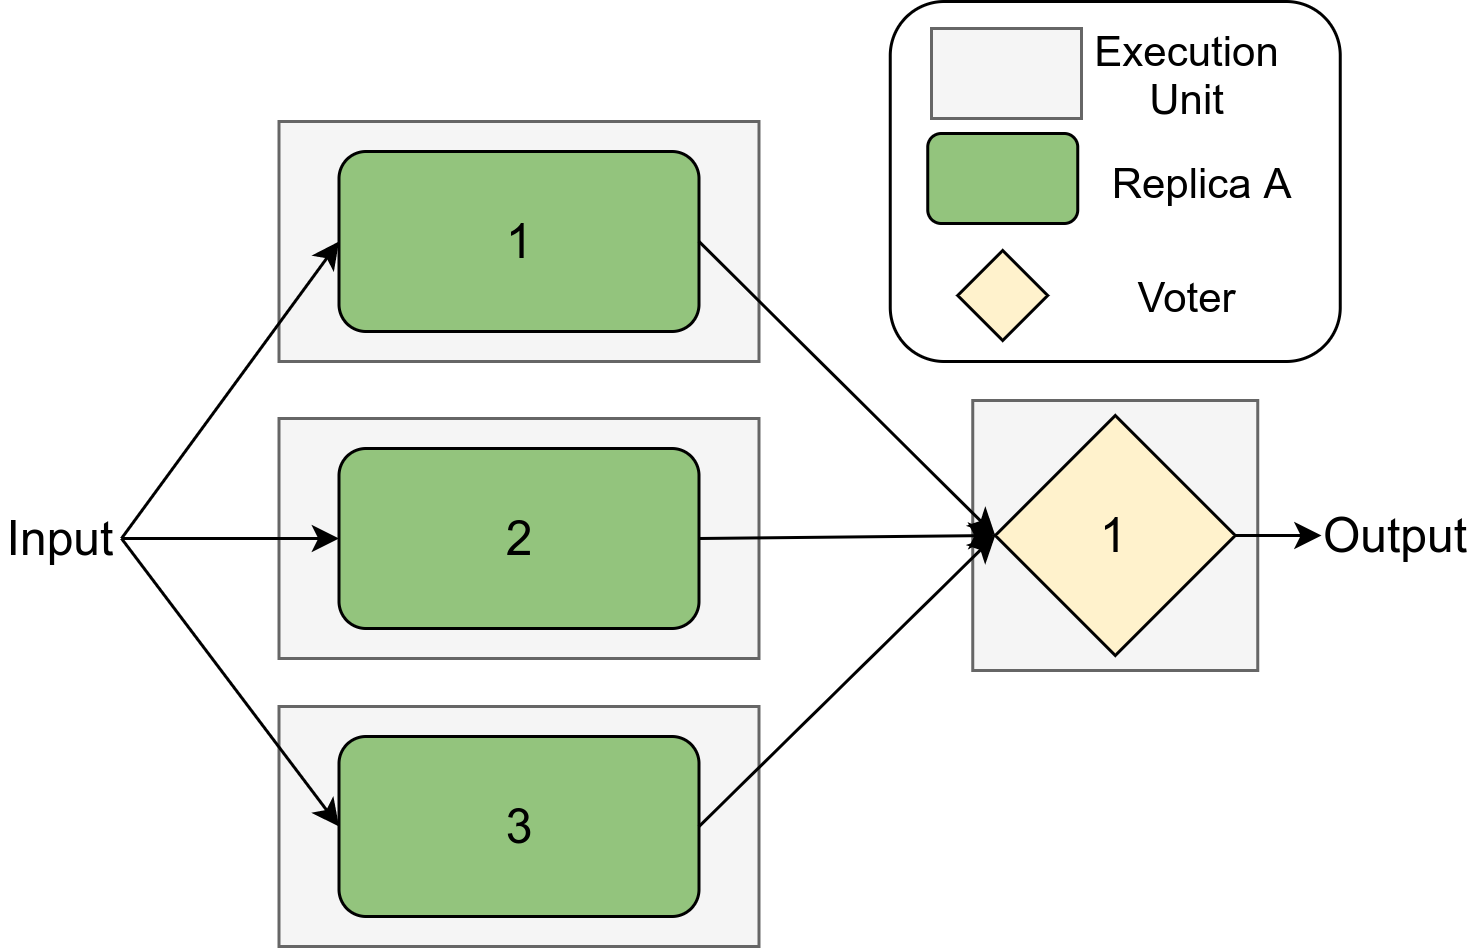
\includegraphics[width=0.75\linewidth]{images/Classical2OO3}
	\caption{Classical 3-out-of-2 redundancy, also known as \glsentryfull{TMR}. Three replicas are simultaneously reading and processing an input in a redundant way. A voter collects these redundant results and performs a majority voting to produce a final output.}
	\label{fig:Classical2OO3}
\end{figure}

One of the most common versions of \gls*{MOON} systems is \gls*{TMR} as shown in~\autoref{fig:Classical2OO3}.
In \gls*{TMR}, three replicas are receiving the same input and performing the same work in parallel.
A voter collects the individual outputs and reduces them to a single system output based on majority voting.
The system output must qualify the characteristic that at least two out of the three replicas agree on this output.
This allows the entire system to still produce a correct output even in the presents of a faulty replica.
All replicas, as well as the voter, are running on individual execution units.

Instead of having one voter that decides about the final result, the calculations could be modularized and votings on intermediate results could be made.
This would have the benefit of masking intermediate faults and not letting them influence further calculations.
An example of how this could be achieved is depicted in~\autoref{fig:IntermediateVoting}.
\\

The biggest weakness of \gls*{TMR} is the voter, because it marks a single point of failure.
Therefore, the voter's reliability in the system has to be high compared to the remaining replicas, because the entire system's reliability cannot be higher than the voter's reliability.
There is a lot of research for making voters more reliable, one of which being Arifeen \etal, who proposed a highly reliable hardware voter~\cite{ArifeenFaultTolerantTMR}.
An alternative to voters are consensus algorithm, where all components, not only a single voter, are involved in deciding about the system's output value~\cite{lamport2001paxos}.
While not having a single point of failure anymore, consensus approaches typically introduce a communication overhead and lead to rigid configurations~\cite{GamerIncreasingMOON}.

\begin{figure}[!hb]
	\centering
	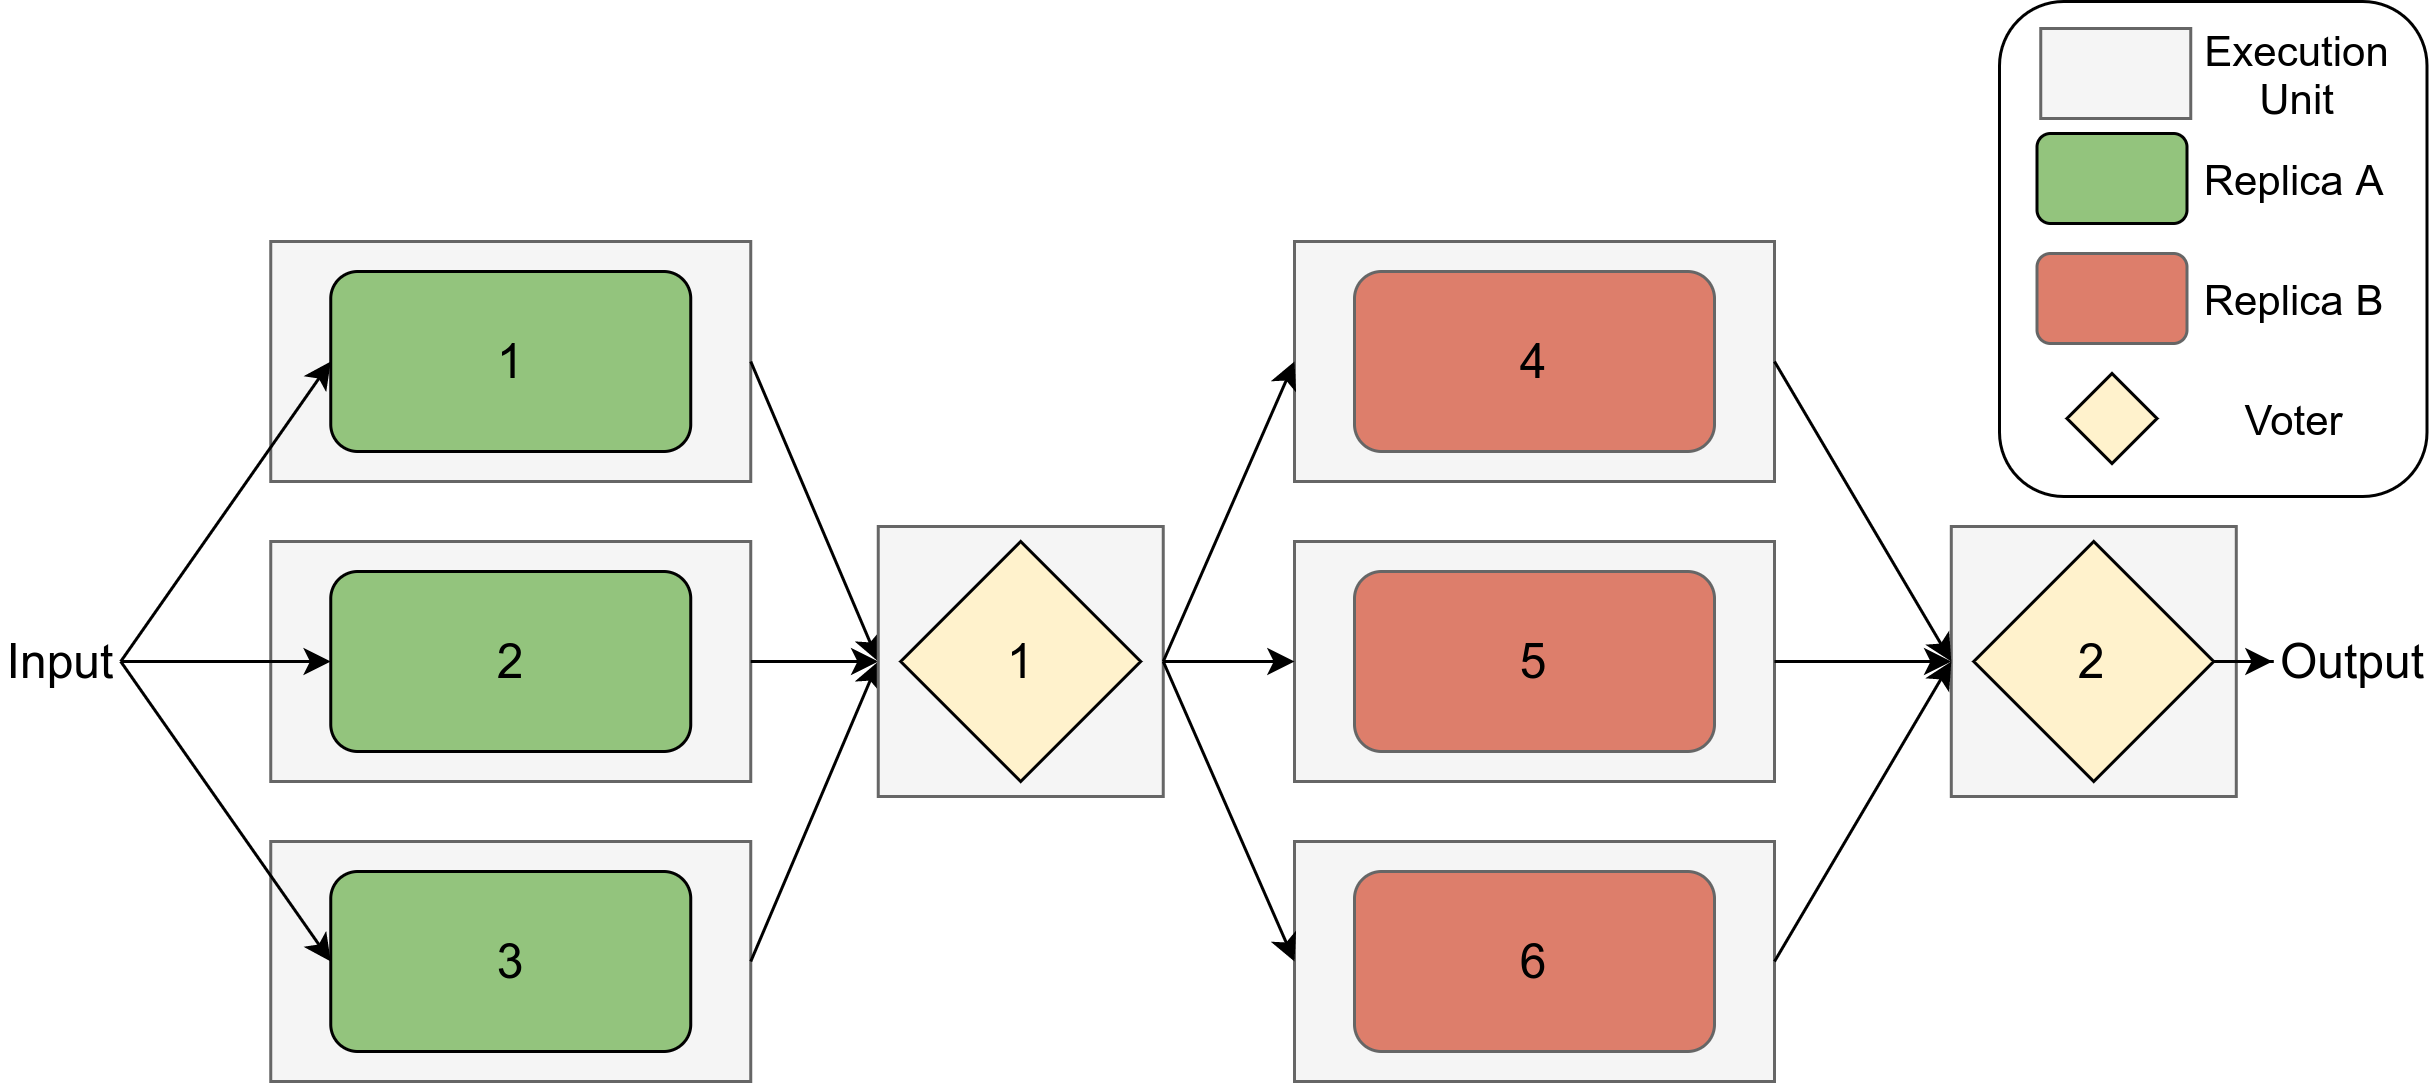
\includegraphics[width=0.75\linewidth]{images/IntermediateVoting}
	\caption{Intermediate voting could be applied to reduce the effect of partial results on the final output. Another benefit of this approach is its pipelined fashion, which improves the overall system throughput.}
	\label{fig:IntermediateVoting}
\end{figure}

\paragraph{Standby Redundancy}
\begin{figure}[!hb]
	\centering
	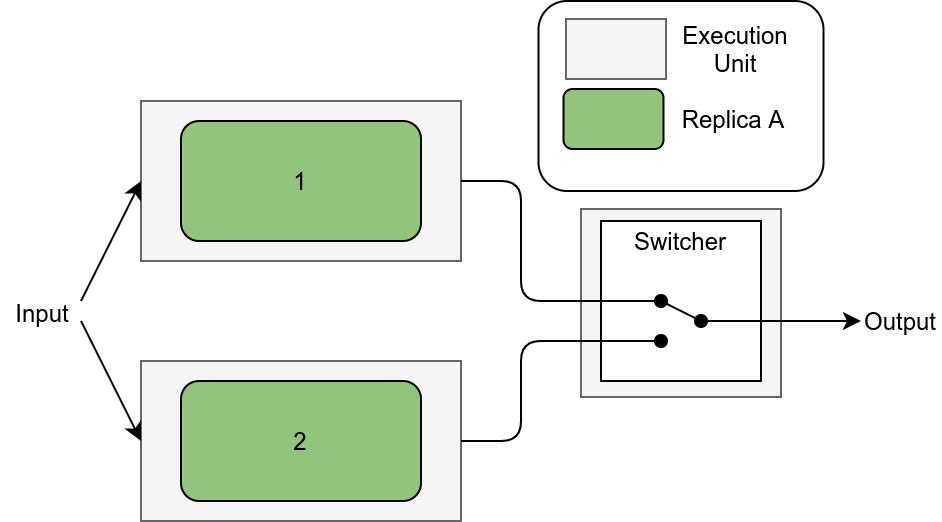
\includegraphics[width=0.75\linewidth]{images/ActiveSelectionRedundancy}
	\caption{With standby redundancy, a system can recover from individual component errors by replacing faulty components. Therefore, a switcher component performs error detection operations and delegates control over the output to the component it considers to be the most trustworthy.}
	\label{fig:StandbyRedundancy}
\end{figure}

As stated above, standby redundancy is an example of active hardware redundancy and builds on the concept of error detection, location and recovery.
If an individual component experiences a fault, the resulting error and faulty component would need to be located so that the system can recover from the error by replacing the faulty component with a spare.
This concept is depicted in~\autoref{fig:StandbyRedundancy}, where two replicas are used, one as a primary and one as a secondary component.
A switching element observes the active component and, when no error is detected, provides control about the system's output to the active component.
As soon as the switching element detects an error, it excludes the active component from the system and transfers control about the system's output to the secondary component, which thereby becomes the active component.
When the secondary component is already running when the switching happens, this is called hot standby redundancy.
When the secondary component needs to be turned on before it can be used as the active component, this is called cold standby redundancy.

\subsection{Software Redundancy}
One speaks of software redundancy when the redundancy concepts or error detection methods are implemented in software.
Examples for software redundancy are heartbeat messages to validate a component's accessibility, component-checking, or software voters.
In component-checking, a software or hardware program is used to monitor and validate a component's hardware, for example its memory, its clock, or its \gls*{CPU}.
A \abr{CPU}, for example, can apply redundant hardware for self-testing and fault-secureness~\cite{SelfCheckingProcessorDesign}.
While self-testing allows the detection of faults, self-secureness ensures that no fault can lead to an undetected error.
Thereby, it can be qualified whether a specific component's output can be considered valid or not.
This state is summarized into the term \texttt{internal consistency}.

\begin{definition}
A system or a component is said to be internally consistent, when any failure of this component is not based on a fault of its internal hardware.
A system's or component's internal consistency can be determined by component checking mechanisms.
\end{definition}

By implication, when a system is internally consistent any system failures can only be introduced by external causes - such as network delays, errors during data transmission, or defects in the inputs.

Further, voting or consensus algorithms can be implemented in software.
Similar to homogeneous and diverse hardware redundancy, diverse implementations of the same software can be used to reduce the effect of faults in a software.
The concept of diverse software programs is summarized under the term N-version programming, where a software program, which is based on the same specification, is developed by separate programmers~\cite{BarryFaultToleranceAnalysis}.

\subsection{Information and Time Redundancy}

\begin{figure}[!hb]
	\centering
	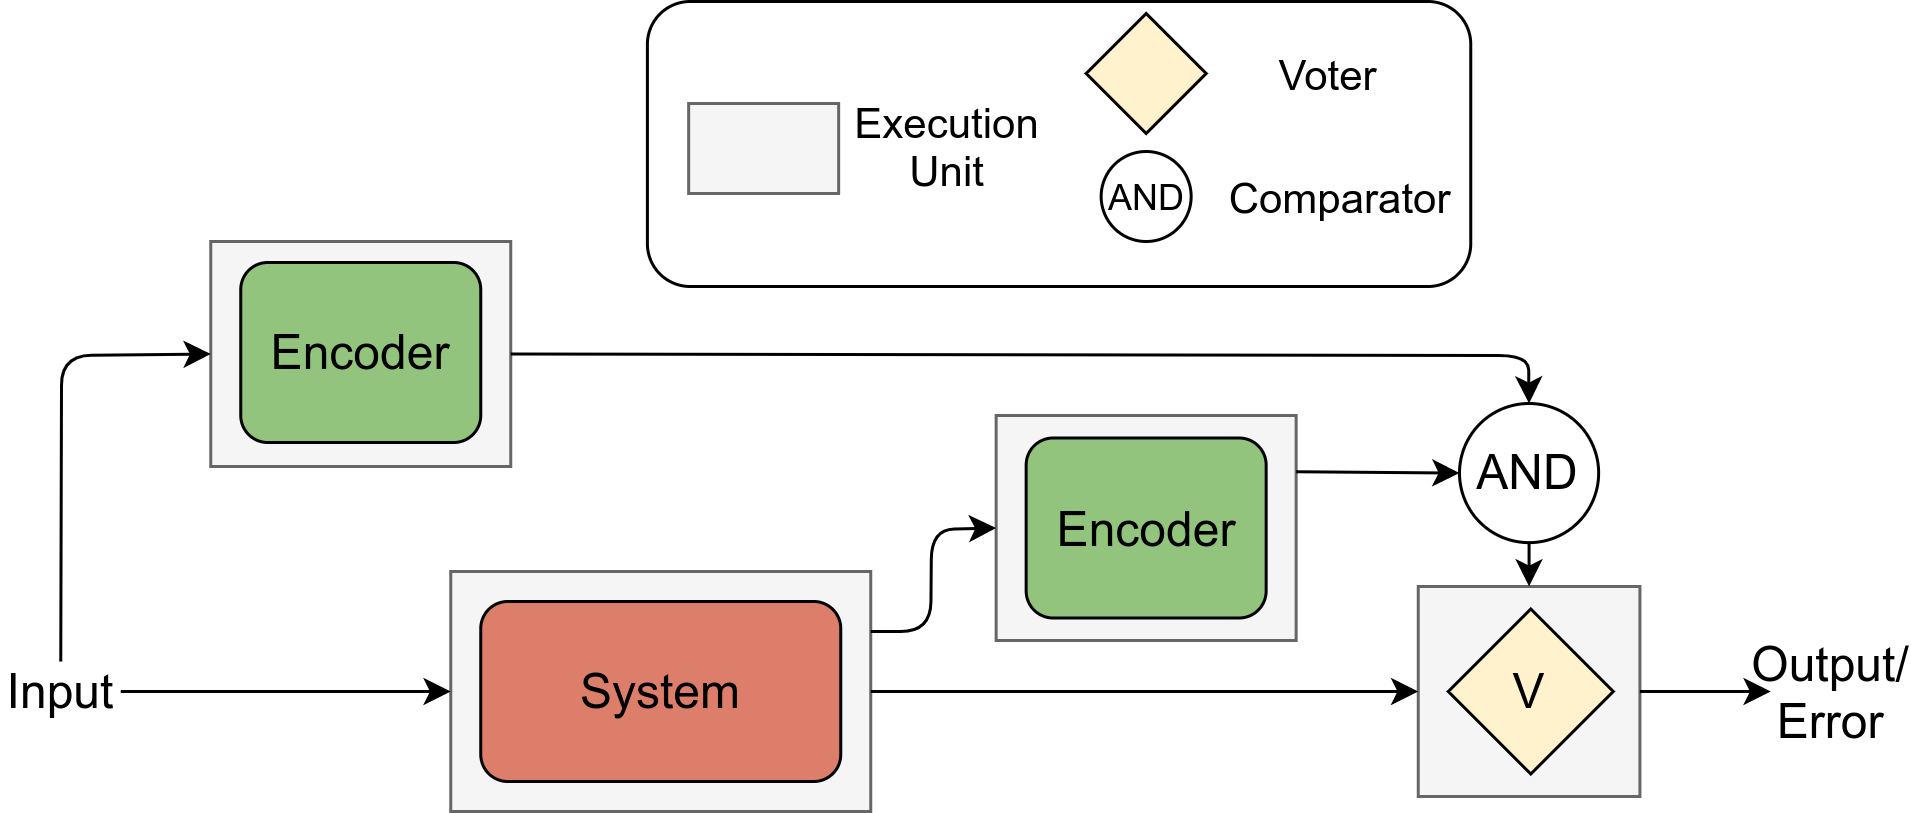
\includegraphics[width=0.75\linewidth]{images/ECC}
	\caption{\glsentryfull{ECC} applies both time and information redundancy. An encoder is used to encode both input and output of a system (time redundancy). This encoded information is used in addition to the actual data (information redundancy). The encoder function needs to be chosen to that possible outputs can be derived from it~\cite{Su2005ECC}. An exemplary encoding that fulfills these characteristics are Hamming codes~\cite{HammingCodes}.}
	\label{fig:ECC}
\end{figure}

The addition of redundant information can allow the detection, masking and recovery from faults~\cite{BarryFaultToleranceAnalysis}.
Examples for information redundancy include Hamming codes~\cite{HammingCodes}, checksums or information duplication.
In Hamming codes, one or multiple parity bits are attached to the data bits so that defects in the transmitted information can be detected.
Additionally, Hamming codes also allow to locate and correct errors in a bitstream.
Information- and time redundancy can be either implemented in software or in hardware using self-checking circuits.
John F. Wakerly argues that, when a system is non-transforming, the applied circuit is automatically self-checking~\cite{SelfCheckingProcessorDesign}.
He further compares different error-detection codes and provides self-checking hardware designs.
All information redundancy concepts share that they somehow encode redundancy into the transmitted data that can later be decoded.
\\

Another way of adding redundancy is to perform the same operation multiple times at different points in time.
This concept is called \texttt{Time Redundancy} and has the benefit that it does not necessarily require additional physical components.
Thereby, permanent faults in a system can be detected.

\autoref{fig:ECC} depicts an example of a combination of information and time redundancy using \gls*{ECC} techniques.
Hereby, an encoder encodes the input and transmits this redundant information together with the input data.
After the system produces an output based on its input information, the output is also encoded and afterwards compared to the encoded input.
When there are anomalies between the system's input and its output, safety operations can be initiated.
The encoding function must be chosen so that it allows the detection of faults in the system.
In an exemplary case, where each input allows two possible outputs, the encoding function could generate two numbers for each input.
These two numbers are redundantly transmitted with the input.
The system's output is further encoded with the same encoding function, which generates an identification number for the generated output.
In a final step, it is verified whether the output's identification number corresponds with one of the input's two possible outputs.

\section{Related Work}
\paragraph{Redundancy to enhance Safety.}
Alapan Chakroborty demonstrates a development process of a reliable, safe and fault-tolerant system using redundancy methods by an example of railway signaling~\cite{ChakrabortyFaultTolerantRailway}.
He argues, that every fault tolerant system needs to build upon real-time software solutions.
This requires both logical, as well as timing correctness, which can only be achieved by correct redundancy management such as fault propagation, synchronization and consensus among replicas.
At a fail-safe design's heart lies fault identification, masking and recovery.
Therefore, in a first step, each redundant design should be subdivided into redundant elements that are not affected by any fault from outside the element.
Chakroborty calls these redundant elements \glspl*{FCR}.
As a second step, he proposes to define interface between the \glspl*{FCR} so that they do not interfere with each other.
These two steps form a necessary precondition to be able to predict the probability of failures in the system.

In order for the system to reduce redundant results to a single result and to mask failures, the concept of voting is demanded.
Voting, as Chakraborty claims, requires the \glspl*{FCR} to be in identical states, to provide all redundant hardware with the same input and to ensure a real-time concurrent operation of the same computations on each \gls*{FCR} for synchronization.
Finally in the work, the shown method is performed on developing a railway signaling system.

An overview about possible redundancy concepts for the railway domain is provided by Bemment \etal~\cite{BemmentEvaluationOfRedundancy}.
They further made a cost, benefit and performance analysis for each presented concept.
\\

In my work, the concepts proposed by Bemment \etal are extended based on the steps by Chakraborty and by using and evaluating the feasibility of \gls*{DDS} for redundancy in the railway context.
Normally, as Bemment \etal pointed out, an in depth redundancy evaluation towards safety and reliability can only be made for well defined use cases where hazards, risks and potential accidents are know.
In my work, however, only the intrinsic safety in examined, which can be done theoretically without doing an exact risk analysis.
For further evaluations, an overview about about possible accidents in railway is given by~\cite{ERTMSRailwayAccidents}.
\\

\paragraph{Software development in the railway context.}
The CENELEC 50128 standard is a norm for software creating processes for railway applications, so that the build software can be considered safe.
The 2011 version of CENELEC 50128, as well as resources needed to achieve a set level of assurance, are presented by Jean-Louis Boulanger~\cite{BoulangerStandards}.
Conducting a CENELEC 50128 conform design process for all software artifacts created in this thesis is outside of its scope.
However, each software intended to be used in railway practice should pass the CENELEC 50128 norm.
\\

\begin{table}[h!]
	\begin{center}
		\caption{\glsentryfull{QOS} policies that affect the communication overhead (o) or the communication time (t). Each \abr{QOS} policy can either be applied to \texttt{DataWriters} (DR), \texttt{DataReaders} (DR), \texttt{Topics} (T), or \texttt{Publishers} (P).}
		\label{tab:qos_garciavalls}
		\begin{tabularx}{\textwidth}{|l|l|X|}
			\hline
			\textbf{QoS policy} & \textbf{Entity} & \textbf{Description}\\
			\hline \hline
			Deadline (t) & DR \& DW & Maximal expected elapsed time between arriving data samples or instances. Max committed time to publish samples or instances.\\
			\hline
			Reliability (o) & DR \& DW & Global policy that specifies whether or not data will be delivered reliably. It can be configured on a per DataWriter/-DataReader connection. \\
			\hline
			History (o) & DR \& DW & Stores sent or received data in cache. It affects the Reliability \gls*{QOS} policy. \\
			\hline
			Resource Limits (o) & DP & Limit to the allocated memory. It limits the queue size for History when the Reliability protocol is used. \\
			\hline
			Latency Budget (t) & T \& DR \& DW & Indication on how to handle data that requires low latency. Allow specification of maximum acceptable delay from time the data is written to the time the data is received by the subscriber. \\
			\hline
			Time based Filter (t) & DR & Limits the number of data samples sent for each instance per a given time period. \\
			\hline
			Transport Priority (t) & DW & Establishes a given priority for the data sent by a writer.\\
			\hline
		\end{tabularx}
	\end{center}
\end{table}

\paragraph{\abr{DDS} in safety-critical systems.}
The \gls*{DDS} is already successfully deployed in distributed time- and safety critical environments.
One example is given by Bijlsma \etal~\cite{DistributedSafety2020}, who extended the E-Gas layered monitoring concept to handle faults in a distributed and redundant system.
\Gls*{DDS} is applied to facilitate a reliable communication among individual components in the system.
An other example is given by Hadiwardoyo and Gao, who proposed the use of \gls*{DDS} in security cameras for subways using \glspl*{QOS}~\cite{DDSInSubways}.
Song \etal have proposed a system architecture that integrates the \abr{DDS} middleware into real-time embedded systems as well as safety-critical systems and thereby achieved a stable communication time~\cite{SongDDSInRealTimeSystems}.
Their approach has been verified by an \abr{UAV} combat scenario that operates in highly safety-critical scenarios.
Results have shown that the worst case communication time for a one kilobyte payload and a reliable communication \abr{QOS} is around 280 microseconds.

Since Song \etal exerted a topology which is similar to the one used in this work - namely a network switch with a 100~Mpbs Ethernet link for communication and external nodes - their findings can be seen as a affirmation for the approach used in this work.
However, they utilized a different \abr{DDS} implementation, so that their experiments need to be repeated in my case to approve their findings. 
\\

A more general approach of how \gls*{DDS} can be used for enabling communication in distributed as well as time- and safety-critical environments, is given by García-Valls \etal~\cite{GarciaVallsDDSInDistributed}.
They used a design of reading and monitoring sensor data to benchmark the middleware's communication performance with different \glspl*{QOS}.
One of their findings is a summary of \gls*{QOS}-policies that effect the system's communication overhead and communication time.
These are illustrated in~\autoref{tab:qos_garciavalls} and are especially important when examining real-time and mission-critical systems.
The results from García-Valls \etal show that the communication performance remains stable even under heavy load.
Even though they applied a different \gls*{DDS} implementation than I did, the network topology and used hardware are comparable, which renders the results from García-Valls \etal useful for my work.

\paragraph{Time and availability for consensus based redundant systems.}
While redundant and distributed architectures are a typical approach to enhance a system's robustness, they also entail the demand to agree on certain data values, where the computations are based on.
Consensus algorithms are a way for components to coordinate and come to an agreement.
However, consensus algorithms also introduce a performance overhead, whose effects on the system's response time have been investigated by Sakic and Kellerer~\cite{SakicTimeInConsensus}.
Their studies focused on \abr{SDN} systems and \texttt{Raft}~\cite{RaftConsensusPaper}, a distributed consensus algorithm that takes care of data replication and leader election.
Results show that a system's response time in case of a random replica failing is linked to the probability of the leader being effected because this would entail a leader election process.
Eventually, in the studies from Sakic and Kellerer after one second, the cluster is almost guaranteed to deliver a response, even in the case of a random replica failing.
The situation looks different for combined correlated hardware and software failures, where only around 20\% of the systems respond a result after one seconds, when more than half of the replicas are affected.
In order to address this problem, Sakic and Kellerer propose a watchdog mechanism, which drastically increased the response probabilities in their experiments.

Based on the work from Sakic and Kellerer, the availability and response time for an actual system need to be evaluated in this work.
Further, the watchdog concepts should be kept in mind as it has a high impact on the system's response time in case of individual component failures.
    \chapter{Systems Evaluation}
\label{chptr:evaluation}



%In this chapter, an example scenario and its requirements are presented.
%Therefore, a risk analysis is made, a data model is presented and a high level analysis towards reliability and safety is conducted.
%Finally, different possible system patterns are presented and compared based on their reliability, practicability and comparability with the \gls*{DCPS}.

\section{Scenario Description}

\subsection{High-Level Risk Analysis}

\section{System Design and Comparison}



\iffalse

In this chapter, typical system architectures for solving highly safety-critical tasks are presented and discussed.

One way of building a dependable system, even out of undependable components, is through distribution (Source ReliabilityEngineering Slides).
This is because the failure of one individual component in a distributed system does not affect the remaining component's dependability.
However, if the failing component was responsible for a crucial system function, then a single failure can lead to a failure of the entire system.
A commonly applied technique for maintaining a system's functionality even when a crucial componant fails is redundancy~\cite{TanenbaumSteen07}.
Therefore, the crucial component's work is performed on multiple components, called replicas, simultaneously.
When one replica fails, the remaining replicas still allow the system to continue its work.

In the following of this chapter, different distributed and redundant system architecture approaches are described and assessed.
At first, redundancy categories that have been proven both in practice and in theory are described, based on~\cite{GeffroyMotetDependableComputing} and~\cite{BarryFaultToleranceAnalysis}.
Afterwards, the most prominent representatives out of the presented redundancy categories are choosen and evaluated based on the requirements made in~\todo{Ref to chapter 1}.
Finally, a decision for the most suitable system architecture for the described use case is compiled.

\section{Redundancy Techniques}


\subsection{Redundancy}

However, adding redundancy also increases the complexity as well as design and building costs of a system.

In computing systems, the two types \texttt{functional}- and \texttt{structural}-redundancy can be found.
While functional-redundancy incorporates a system's external manner, structural-redundancy refers to its internals.

\subsubsection{Functional Redundancy}
Functional redundancy is encoded in the relationship between a system's input and its output.
It allows the system to filter out impossible or unacceptable inputs or outputs.
Functional redundancy is independent of the system's design and implementation and solely depends on its functions.
A way of adding functional redundancy to a system is to structure it into interconnected modules~\cite{GeffroyMotetDependableComputing}.
\todo{Explain this further}

\subsubsection{Structural Redundancy}
For structural redundancy, additional components are added to the system that would be unnecessary, provided all components are working correctly.
Structural redundancy can be applied in software, in hardware or in the time domain~\cite{GeffroyMotetDependableComputing}.
Examples for structural redundancy are:

\paragraph{Standby Redundancy}
In standby redundancy, the redundant components are subdevided into primary and secondary components.
A third component type is required to switch between the primary and secondary components, when required.
The switching step, however, is not possible without any costs and adds an additional point of failure~\cite{PepperlFuchs}.
Standby redundancy is subdevided into cold and hot standby, implicated whether the secondary components are turned off or on while they are not used.

\paragraph{M-out-of-N Redundancy}
Another popular redundancy pattern for industrial applications is \gls*{MOON}-redundancy~\cite{GamerIncreasingMOON}.
Thereby, N individual components are executing the same task simultaneously and all separate outputs are collected.
The system finally generates the overall output by selecting the value where at least M out of the N components agreed on.
This allows the system to generate the right output even if $N-M$ components produced a wrong output.



\todo{Define module composition}

In structural redundant systems, it often happens that multiple redundant outputs need to be reduced to a single system output.
In order to produce a single output out of $N$ individual outputs, a voter or a consensus algorithm could be used.

\paragraph{Voter} 
A voter is an entity that collects the components individual outputs and performs a voting algorithm to combine them to a single output.
The voter approach has the benefit that it is fast and easy to implement.
For voter based systems, Chow and Willsky argue that system output's residual generation can be done by simply comparing outputs of redundantly working components~\cite{ChowFailureDetectionSystems}.
However, a voter is a single point of failure and thereby impairs the entire systems reliability and availability.

\paragraph{Consensus} 
A consensus algorithm is applied to reach consensus among the system's individual components in order to agree on a single output value.
This single output value is required to be proposed by at least one component~\cite{lamport2001paxos}.
While not having a single point of failure anymore, consensus approaches typically introduce a communication overhead and lead to rigid configurations~\cite{GamerIncreasingMOON}.


\section{Choosing a System Architecture}







\autoref{fig:Classical2OO3} depicts the most prominent form of passive hardware redundancy, \gls*{TMR}~\cite{BarryFaultToleranceAnalysis}.


The weakness of \gls*{TMR} is the voter, because it marks a single point of failure.
Therefore, the voter's reliability in this system has to be very high compared to the three replicas, because the entire system's dependability cannot be higher than the voter's dependability.
A solution to this problem would be to increase the number of voters.
However, having multiple voters would also lead to having multiple outputs and would require an additional step to combine the individual outputs to a final output, being a new single point of failure.

It is assumed that all replicas follow the exponential failure law.
Based on \autoref{eq:expFailureLaw} and \autoref{eq:reliabilityMOON} follows for the replicas reliability
\begin{equation}
R_{2oo3}(t) = \sum_{i = 2}^3 {3 \choose i} * (e^{-\lambda t})^i * (1 - e^{-\lambda t})^{3 - i}
\end{equation}

%
%
%


\section{Error Checking and Correction}



%Throughput can be increased by combining the parallel and serial pattern in a pipelined way.
%This also has the way that it adds functional redundancy to the system~\cite{GeffroyMotetDependableComputing}.


\todo{Define several candidate designs}
\todo{Analyze candidate designs}


\fi

    \chapter{Implementation}
\label{cpt:Implementation}

In this chapter, a practical implementation of a consensus-inspired redundant architecture is presented.
The applied consensus algorithm is based on the concepts of \texttt{Raft}.
This implementation's aim is to showcase the practicability and performance of a redundant architecture that applies \abr{DCPS} concepts for finding a consensus in an \abr{ETCS} context, even in the presence of individual component failures.
\\

At first in this chapter, the structure of the implemented system is presented.
Therefore, the utilized hardware, the network topology, and the software structure are described.
In the second section, the way the system manages its state is explained.
Afterward, the system's behavior is outlined in two steps.
First, a leader election algorithm - the basis for further processing - is shown.
Second, the decision-making algorithm, which is based on redundant computation and majority voting, is presented.
Finally in this chapter, methods for system recovery are described.
These include an active hardware redundancy approach as well as a hardware watchdog.

\section{System Structure}

\begin{figure}[!hb]
	\centering
	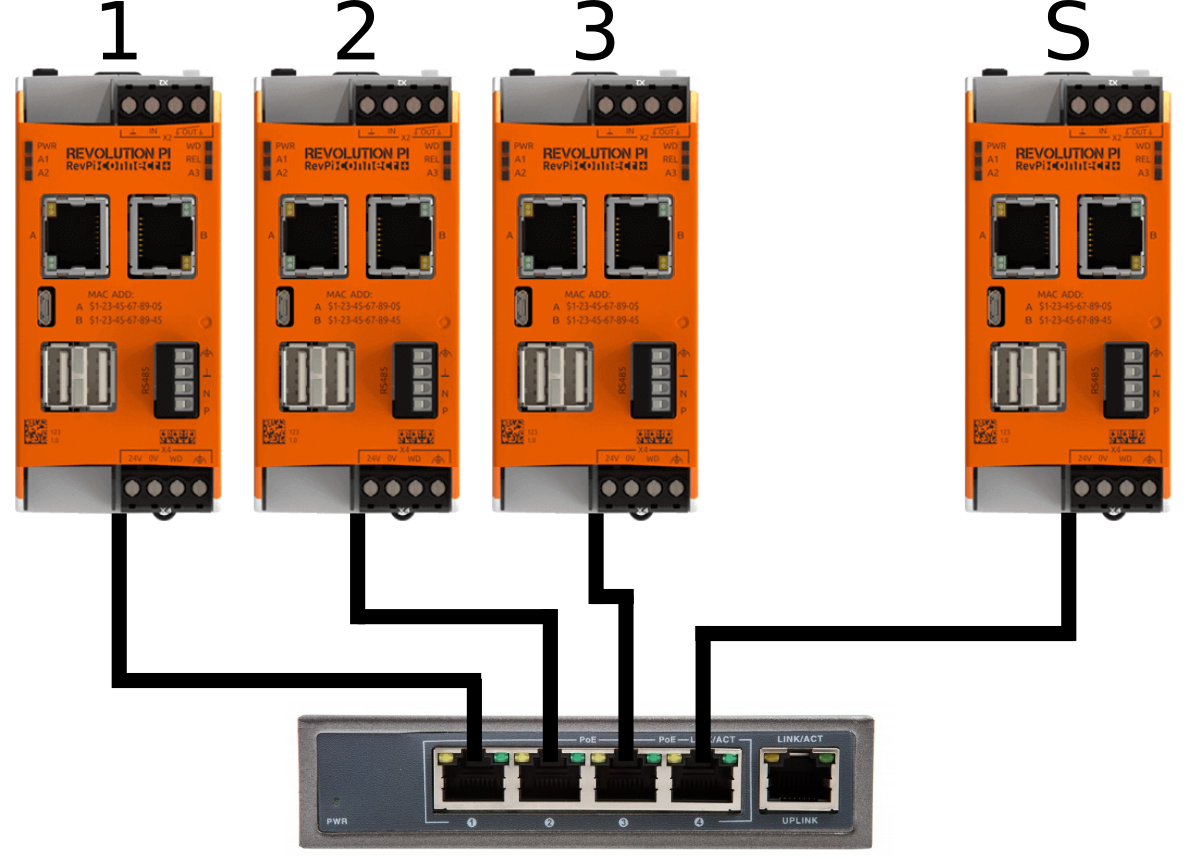
\includegraphics[width=0.8\linewidth]{images/setup}
	\caption{Three \textit{Revolution Pi Connects} make up the redundant system which is implemented in the course of this thesis. The replicas are interconnected via a network switch. A fourth \textit{Revolution Pi Connect} acts as a spare unit that is activated upon a failure of any other replica.}
	\label{fig:SystemSetup}
\end{figure}

\begin{figure}[!hb]
	\centering
	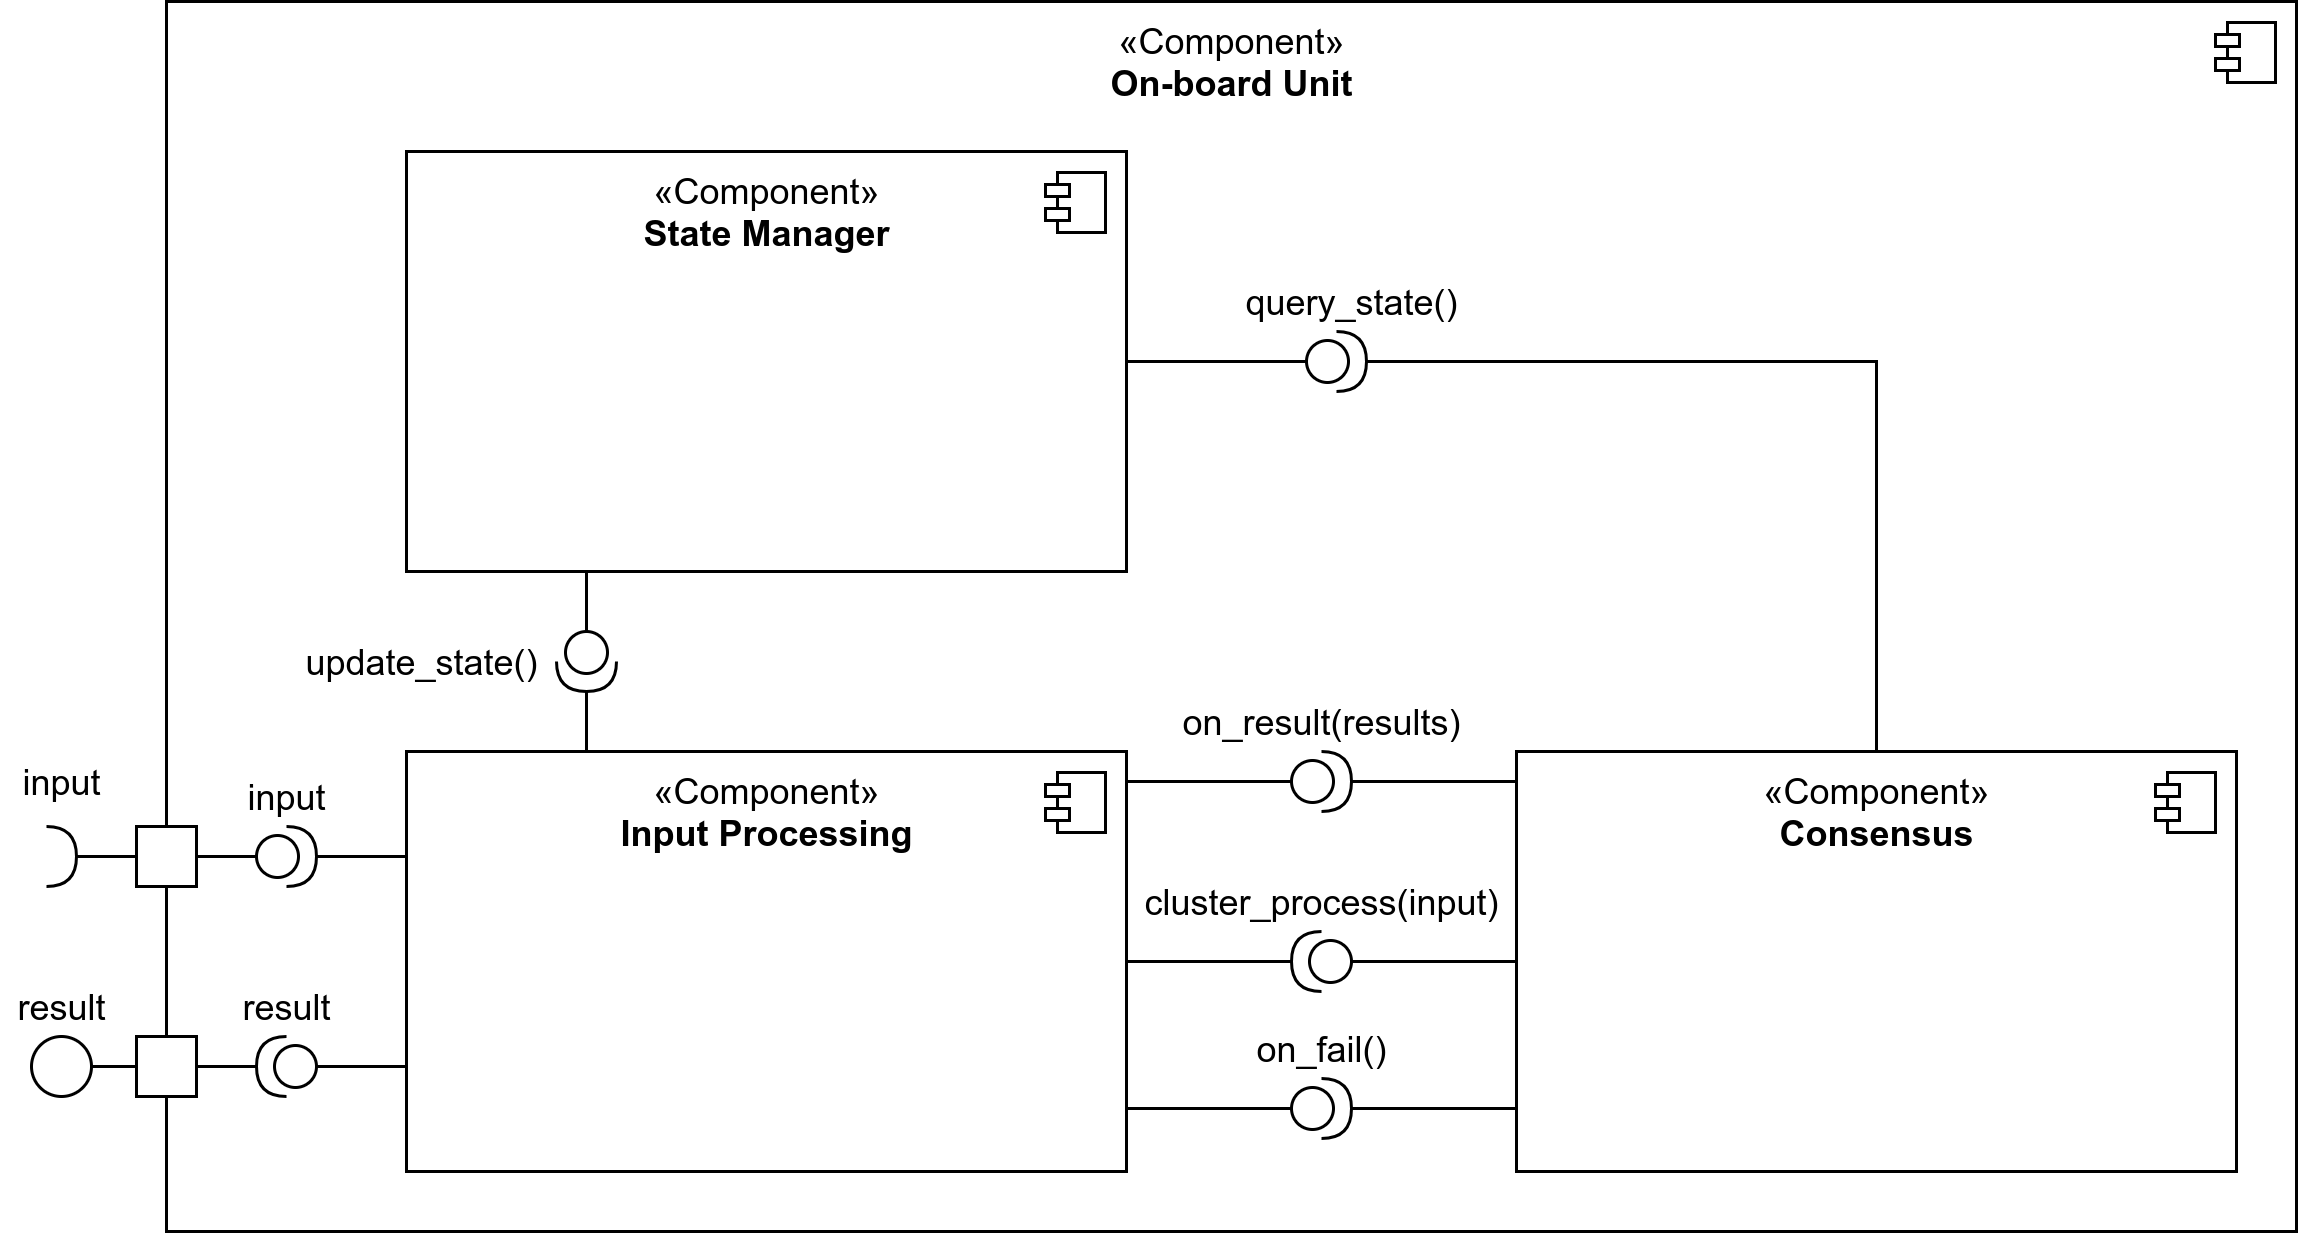
\includegraphics[width=0.9\linewidth]{images/Components}
	\caption{The on-board unit's program, which runs on each replica, consists of three major components. The \texttt{input} processing reads inputs and performs the voting. While the \texttt{state manager} component administers the system's global state, the \texttt{consensus} component ensures that a leader is present in the system and provides an interface to perform redundant processing and voting.}
	\label{fig:SystemComponents}
\end{figure}

The system's setup to implement the architecture from~\autoref{fig:ThreeRepConsensusDDS} is depicted in~\autoref{fig:SystemSetup}.
Four replicas are interconnected via a network switch.
While three replicas are operating in a \abr{TMR} setup, the fourth is used as a spare unit that can be activated on demand, for example when another replica failed.
Each replica is represented by a \textit{Revolution Pi Connect}, an open-source \abr{PLC} that builds upon a Raspberry Pi and is developed by \texttt{Kunbus}.
As such, it features a Broadcom BCM2837 quad-core ARM Cortex A53 1.2 GHz \abr{CPU} and 1 GB \abr{RAM}.
The used \abr{OS} is an extended \textit{Raspbian} \abr{OS} that has been patched with real-time support.
The solution is implemented in the C-programming language and makes use of the C \abr{API} of \textit{Votex OpenSplice DDS} by \texttt{ADLINK}.
\\

A general outline of the system's structure is provided in~\autoref{fig:SystemComponents}.
The \texttt{Input Processing} component provides an interface to the system's environment.
Information about \abrpl{MA}, linked balises, and balise telegrams can be transferred to the system via the \textit{input} interface.
Via the \textit{result} interface, the votet result for a corresponding input is presented.
\\

The system distinguishes between two message types.
Informative messages, such as a \abr{MA} or a set of linked balises, alter the system's state.
Upon receiving an informative message, the system's leader integrates the information into the system's global state by utilizing the \texttt{State Manager} component's \textit{update\_state()} functionality.
Critical messages, such as balise telegrams, require the system to make a decision.
After receiving a critical message, the system's leader applies the \texttt{Consensus} component to generate a system-wide decision.
Every replica generates a decision based on the system's global state.
When the decision-making succeeded, the \textit{on\_result} callback is called.
Otherwise, \textit{on\_fail} would be invoked.
\\

Because the network is arranged in a star network, the network switch makes up a single point of failure.
For safety-reasons, a fully connected network would be the better choice.
However, since the software implementation is independent of the applied network topology, a star network was chosen due to cost reasons.

The communication channel is implemented via \textit{Ethernet} and no information redundant communication channel is applied in this demonstration.
Further, no N-version programming is applied, which means that each replica runs the same software implementation.
In addition, it is assumed that all replicas' hardware functions as intended.
When this cannot be expected, component checking mechanisms, such as self-checking hardware, can be applied.
In order to build a highly secure system, the mentioned compromises need to be further addressed.

\section{System State}
\label{sec:stateManager}
It is mandatory for the replicas in the distributed system to produce deterministic results and to have access to the most recent global system state.
The system's state is stored as a global state in \abr{DDS} state topics and consequently managed by the middleware.
This ensures that all replicas can operate on the most recent system state and no replica becomes outdated.
Only the system's leader is permitted to alter the system's state, all other replicas have read-only access.
Three \abr{DDS} state topics make up the global system state.
\\

The currently valid \abr{MA} is stored in the \texttt{MovementAuthority} topic.
A \abr{MA} is transmitted to the system before a journey starts and is valid for an entire journey.
Hence, a \abr{MA} is stored in an enduring state topic (see~\autoref{tab:stateQOS}) so that it is reliably transmitted to all replicas.
Further, the currently valid \abr{MA} is transmitted to late joining replicas.
\\

The set of linked balises is managed by the \texttt{LinkedBalises} topic.
As for \abrpl{MA}, a set of linked balises is assigned once and valid for an entire journey so that an enduring state topic is used.
Further, because multiple balise instances are managed via this topic, an unique identifier is used to distinguish the balises.
\\

The train's position and speed are stored in the \texttt{TrainState} topic.
Three variables are used for the position.
One encodes the estimated position and two delimit an interval, the so-called confidence interval, that contains the train's actual position.
A confidence interval is required because position measuring instruments can have inaccuracies.
The topic further contains information about whether the train is moving.
Because the state data is updated periodically and frequently, it is managed as a volatile \abr{DDS} state topic.
\\

The different state topic's data is read and written like any other \abr{DDS} topic.
However, before starting a new journey, it is mandatory to ensure that any information about previous \abrpl{MA} and linked balises is no longer accessible.
In order to circumvent this situation beforehand, any data on the \texttt{MovementAuthority} and \texttt{LinkedBalises} topic is disposed before new data is written.

\section{System Behaviour}

In this section, the components used for processing inputs are described.
The basis for further processing is the election of a system leader.
Upon receiving a critical input, a system-wide decision is made based on redundant computation.
Therefore, a leader election algorithm that applies a \abr{DCPS} communication pattern and follows the concepts of \texttt{Raft} is presented.
Afterward, an algorithm for creating a voted decision based on redundant results is presented.
For both algorithms, safety and timing considerations are described.
\\

For the application to notice that data samples are available on topics, \abr{DDS} \texttt{WaitSets} are used.
\texttt{WaitSets} are preferred over \abr{DDS} \texttt{Listeners} because they are state-based rather than event-based, which means they trigger as long as the system is in a specific state rather than when an event is triggered.
Thereby, \texttt{WaitSets} ensure that no available data is missed.
Further, by using \texttt{WaitSets}, complete control over the application is managed by the application itself.
If \texttt{Listeners} had been used, the application logic that should be executed upon the event would be managed by the middleware.
As a result, the application logic cannot block the application logic.
\\

As depicted in~\autoref{fig:ThreeRepConsensusDDS}, the replicas are communicating via \abrpl{RPC} that are represented by \abr{DDS} event topics.
Although only one topic has been used for each \abr{RPC} so far, a distinct \abr{DDS} topic for requesting and answering to \abrpl{RPC} is required in practice.
This is because topics in \abr{DDS} need to be in a particular data format.
Thus, an event topic called \texttt{AppendEntriesReply} is used to answer to messages send via \texttt{AppendEntries}.
The same applies for \texttt{RequestVote}, whose \texttt{RequestVoteReply}.


\subsection{Leader Election}
\begin{figure}[!hb]
	\centering
	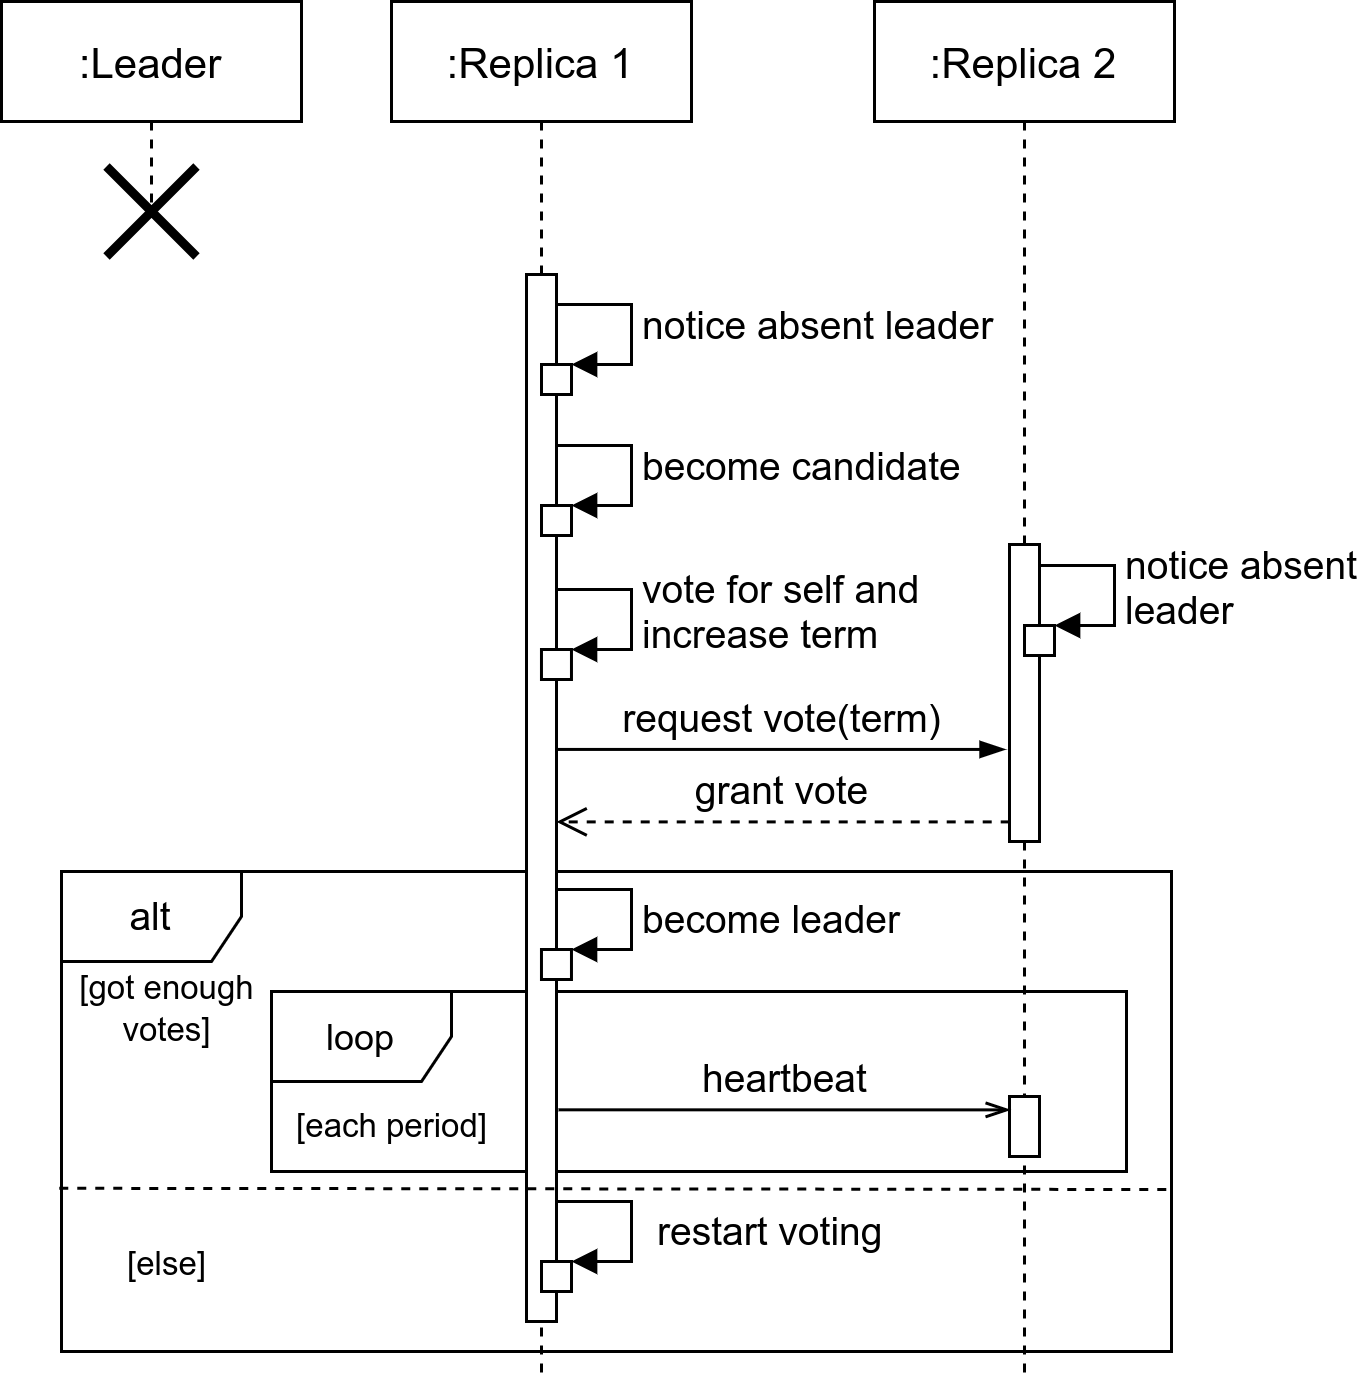
\includegraphics[width=0.75\linewidth]{images/sequence/LeaderElection}
	\caption{When a replica notices that the leader crashed, it becomes a candidate, votes for itself and sends vote requests to all remaining replicas. When enough votes were granted, it becomes the new leader and starts sending heartbeats. Otherwise, it retries to become the leader in the next term.}
	\label{fig:SeqLeaderElection}
\end{figure}

In this section, a consensus algorithm that follows the concepts of \texttt{Raft} and applies the \abr{DDS} publish/subscribe communication pattern is presented.
A consensus algorithm guarantees that there is at most one leader present in the system at a time and that a new leader is elected when there is none present.
The remaining replicas transition to follower mode when they recognize a leader.
Time in \texttt{Raft} is subdivided into \textit{terms}, that each start with a leader election.
When a follower recognizes a missing leader in the system, it starts a new term and promotes to become the new leader. 
Each replica manages its term, its current role, and voting information as a private replica state.
\\

It is the leader's responsibility to inform the remaining replicas about its existence.
Therefore, the leader periodically publishes heartbeat messages onto the \texttt{AppendEntries} topic.
When a replica does not receive a message from a leader for a specific period of time, called the \textit{election timeout}, it promotes to become the new leader.
A high-level overview of a voting process is depicted in~\autoref{fig:SeqLeaderElection}.
Replica 1 notices the crashed leader first and promotes to become the new leader by switching into candidate mode and sending a vote request to each remaining replica.
In the exemplary case in~\autoref{fig:SeqLeaderElection}, replica 2 accepts the vote request and replica 1 becomes the new leader.
It immediately starts sending heartbeat messages afterwards.
\\
In the following, the allocation and the collection of votes will be discussed in more detail.
\\\\

\begin{algorithm}[H]
\caption{Algorithm for vote allocation. Whether a vote gets granted or rejected depends on whether the replica that receives the vote request has already voted for another replica in the voting term.}\label{algo:VoteAllocation}
\SetKwData{Term}{\textit{term}}
\SetKwData{Sender}{\textit{senderID}}
\SetKwInOut{Input}{input}
\SetKwInOut{Output}{output}

\Input{A vote request with a \Term and a \Sender}
\Output{true if the vote for \Sender in \Term was granted, false otherwise}
\BlankLine
\If{\Term $>$ current term}{become follower in new \Term\;}
\If{\Term $==$ current term \textbf{AND} not voted in current term}{grant vote for \Sender\;}
\end{algorithm}

The allocation of votes is shown in~\autoref{algo:VoteAllocation}.
Each replica can only vote for one other replica in every term.
Because the system's state is managed globally by \abr{DDS}, every replica is equally up to date so that vote allocation only depends on the promoting replica's term.
As soon as a vote request is received that has a higher term number than the replica's term, the receiving replica automatically transitions into follower mode.
Afterward, it grants the vote for the promoting replica.
Only a single leader is allowed to be active in a term so that replicas are not allowed to vote for multiple replicas in a single term.
\\

\begin{algorithm}[H]\caption{Algorithm for vote collection. Only votes that were answered in the same term that the vote request was issued are considered. When enough votes are collected, the replica becomes the leader. If a vote was answered in a more recent term, the vote collection gets aborted and the replica becomes a follower.}\label{algo:VoteCollection}
\SetKwData{VoteTerm}{\textit{voteTerm}}
\SetKwData{VoteGranted}{\textit{voteGranted}}
\SetKwInOut{Input}{input}
\SetKwInOut{Output}{output}

\Input{A vote reply with a \VoteTerm and a \VoteGranted flag}
\Output{Transition to either leader or follower state}
\BlankLine

\If{the replica is no candidate anymore}{return\;}
\If{\VoteTerm $>$ term when election started}{
become follower\;
return\;}
\If{\VoteTerm $==$ term when election started \textbf{AND} vote got granted}{
Increase number of granted votes in the election term\;
	\If{got enough votes}{
	become leader\;
	return\;}
}
\end{algorithm}

Whether a promoting replica becomes the new leader depends on the number of accepted vote requests.
For each vote reply received by a promoting replica, it is first checked whether the replica has left the candidate state in the meantime, which makes the entire vote reply irrelevant.
This can, for example, happen when another vote request with a higher term number has been granted while the replica itself waits for incoming vote replies.
Afterward, it is checked whether the term of the processing replica was higher than the term in which the voting was started.
This fact indicates that the promoting replica is outdated, so that should not become a leader and transition into follower mode.
Finally, when the vote got granted and enough granted votes were received, the replica is elected as a new leader for the corresponding term.
The number of necessary voted depends on the total number of replicas in the system.

\begin{figure}[!hb]
	\centering
	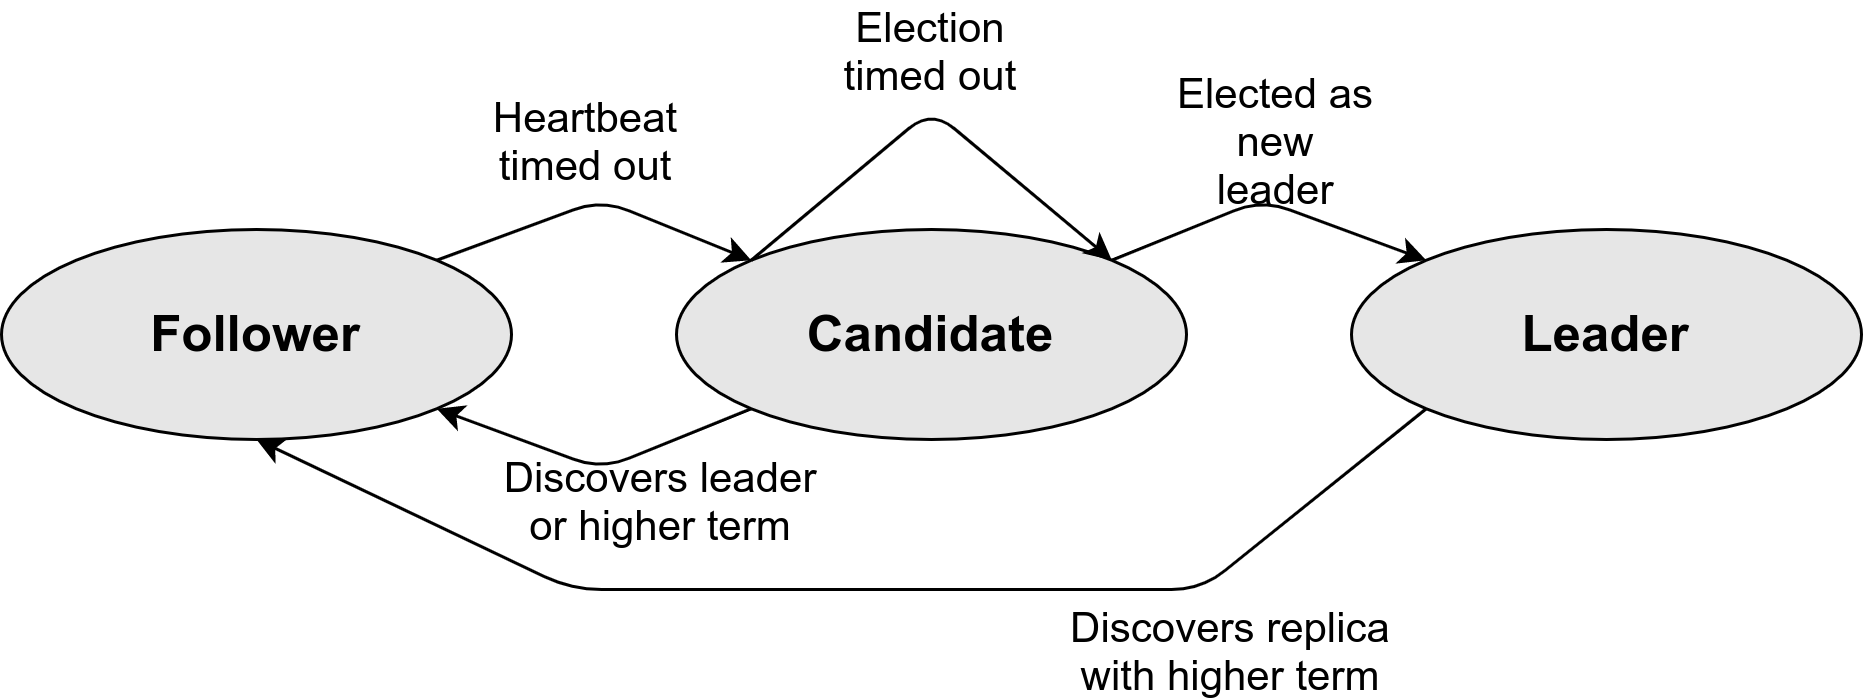
\includegraphics[width=0.75\linewidth]{images/RaftServerStates}
	\caption{Replicas in \texttt{Raft} can be in one of three states. When a follower receives no heartbeat messages from a leader, it starts an election and tries to become the new leader. A replica remains in the candidate state either until it becames the new leader or until it receives a heartbeat from another leader in a higher term. Leaders operate until they fail or until they discover that their term is outdated. This diagram was taken from~\cite{RaftConsensusPaper}}
	\label{fig:RaftServerStates}
\end{figure}


\subsubsection{Safety Considerations}
\label{subsub:raceConditions}

It is crucial for the system's safety that only one leader is present at any time.
Further, it needs to be ensured that a new leader is elected after the previous leader failed and that the system is not without a leader for a specific period of time.
When a leader election is impossible, the remaining replicas must ensure that the train stops.
This can lead to situations where multiple replicas at once take control about the system's output.
Therefore, only the most restrictive output should be taken - in this case stopping the train.
Specialized multiplexing hardware that filters simultaneous outputs can ensure that always the most restrictive output is taken.
Other hardware, such as gravity-controlled switches, can ensure that a train stops when no replica is active at all.
\\

The election algorithm is implemented as a concurrent algorithm.
Because no assumptions about the thread's relative speed can be made, race conditions can occur~\cite{Dijkstra1965}.
In the following, it is described how the algorithm ensures functional correntness with \abr{DDS} features and prevents race conditions.

\paragraph{Functional Correctness}
During the entire time, each replica is in one of three states, namely \texttt{Leader}, \texttt{Candidate} or \texttt{Follower}.
The leader election process can be summarized as transitions and corresponding conditions between these three states, as depicted in~\autoref{fig:RaftServerStates}.
Five requirements can be derived from the figure that must be met by an algorithm that implements \texttt{Raft}'s leader election process:

\begin{enumerate}
\item \textbf{Start Election:} A follower becomes a candidate, increments its term, votes for itself, and sends a message to all other replicas stating that it wants to become the leader.
\item \textbf{End of Election:} A candidate remains in candidate state until it either wins the election, receives information about another leader in the system, or times out.
\item \textbf{Won Election:} A candidate wins the election if it receives votes from a majority of replicas in the same term. Each replica votes for at most one replica in a given term.
\item \textbf{Lost Election:} A candidate loses the election when it receives a message from a leader whose term is at least as high as the candidate's term.
\item \textbf{No Result:} A certain period of time goes by without the candidate winning or loosing the election.
\end{enumerate}

For realizing the leader election algorithm with \abr{DCPS} features, three \texttt{Topics} are required.
The \texttt{AppendEntries} and \texttt{RequestVote} topics are representatives for the corresponding \texttt{Raft} \abrpl{RPC}.
Because data objects managed by \abr{DDS} require a predetermined structure, a dedicated topic for replying to vote requests is required.
Therefore, \texttt{RequestVoteReply} is utilized.

A missing leader is detected by not receiving heartbeat messages for a certain period of time.
This period of time is called \textit{election timeout}.
For implementing an \textit{election timeout}, a \texttt{WaitSet} with a corresponding \texttt{ReadCondition}, that triggers when new data has been published to \texttt{AppendEntries}, is applied.
Further, a timeout is attached to the \texttt{WaitSet} that matches the \textit{election timeout}.
This way, if no heartbeat message is received for the \textit{election timeout} period, an event is triggered.
Although a heartbeat message is a periodic message and a deadline \abr{QOS} could be used to register an absent leader, a timeout is preferred.
This is because a \texttt{WaitSet} with a timeout is required for other messages as well and the deadline \abr{QOS} would require a \texttt{StatusCondition} to be noticed whereby the utilized \abr{DDS} subset would grow.
In order to initiate the voting process, the replica publishes a new vote request to \texttt{RequestVote}.
Because the middleware ensures that data is transmitted to all replicas that subscribed to a topic, the \textbf{Start Election} requirement can easily be solved with \abr{DDS}.
\\

Further, \textbf{No Result} can be resolved by using a \texttt{WaitSet}, called \textit{leaderElection\_WaitSet}, with a corresponding timeout (\textit{leader ready timeout}).
When the timeout expires, the replica starts to wait for heartbeat messages again.
In addition to the timeout, a \texttt{ReadCondition} is attached to the \textit{leaderElection\_WaitSet} that triggers when messages from a leader have been published to the \texttt{AppendEntries} topic.
Thereby, \textbf{Lost Election} is ensured.
By implication, this means that the candidate either won the election for the term, or the election was not successful.
An election was unsuccessful when the timeout attached to \textit{leaderElection\_WaitSet} expires.
Thus, \textbf{Won Election} is partly solved.

In order to fully solve \textbf{Won Election}, each replica needs to collect votes and reply to vote requests, parallel to detecting other leaders and voting timeouts.
The voting part is therefore treated by another \abr{OS} thread, that again makes use of a \texttt{WaitSet}, where two \texttt{QueryConditions} are attached to, one for the \texttt{RequestVote} and one for the \texttt{RequestVoteReply} topic.
Thereby, the replicas can agree to a vote request while the candidate waits for the voting to end.

In the case of a network partition, where one or multiple replicas are separated from the others, split-brain situations with multiple leaders - one for each subnet - could happen.
However, the quorum required for voting prevents multiple replicas in a partitioned network to become the leader and prevent split-brain situations from leading to system failures.

\paragraph{Absence of Race Conditions}

\begin{figure}[!hb]
	\centering
	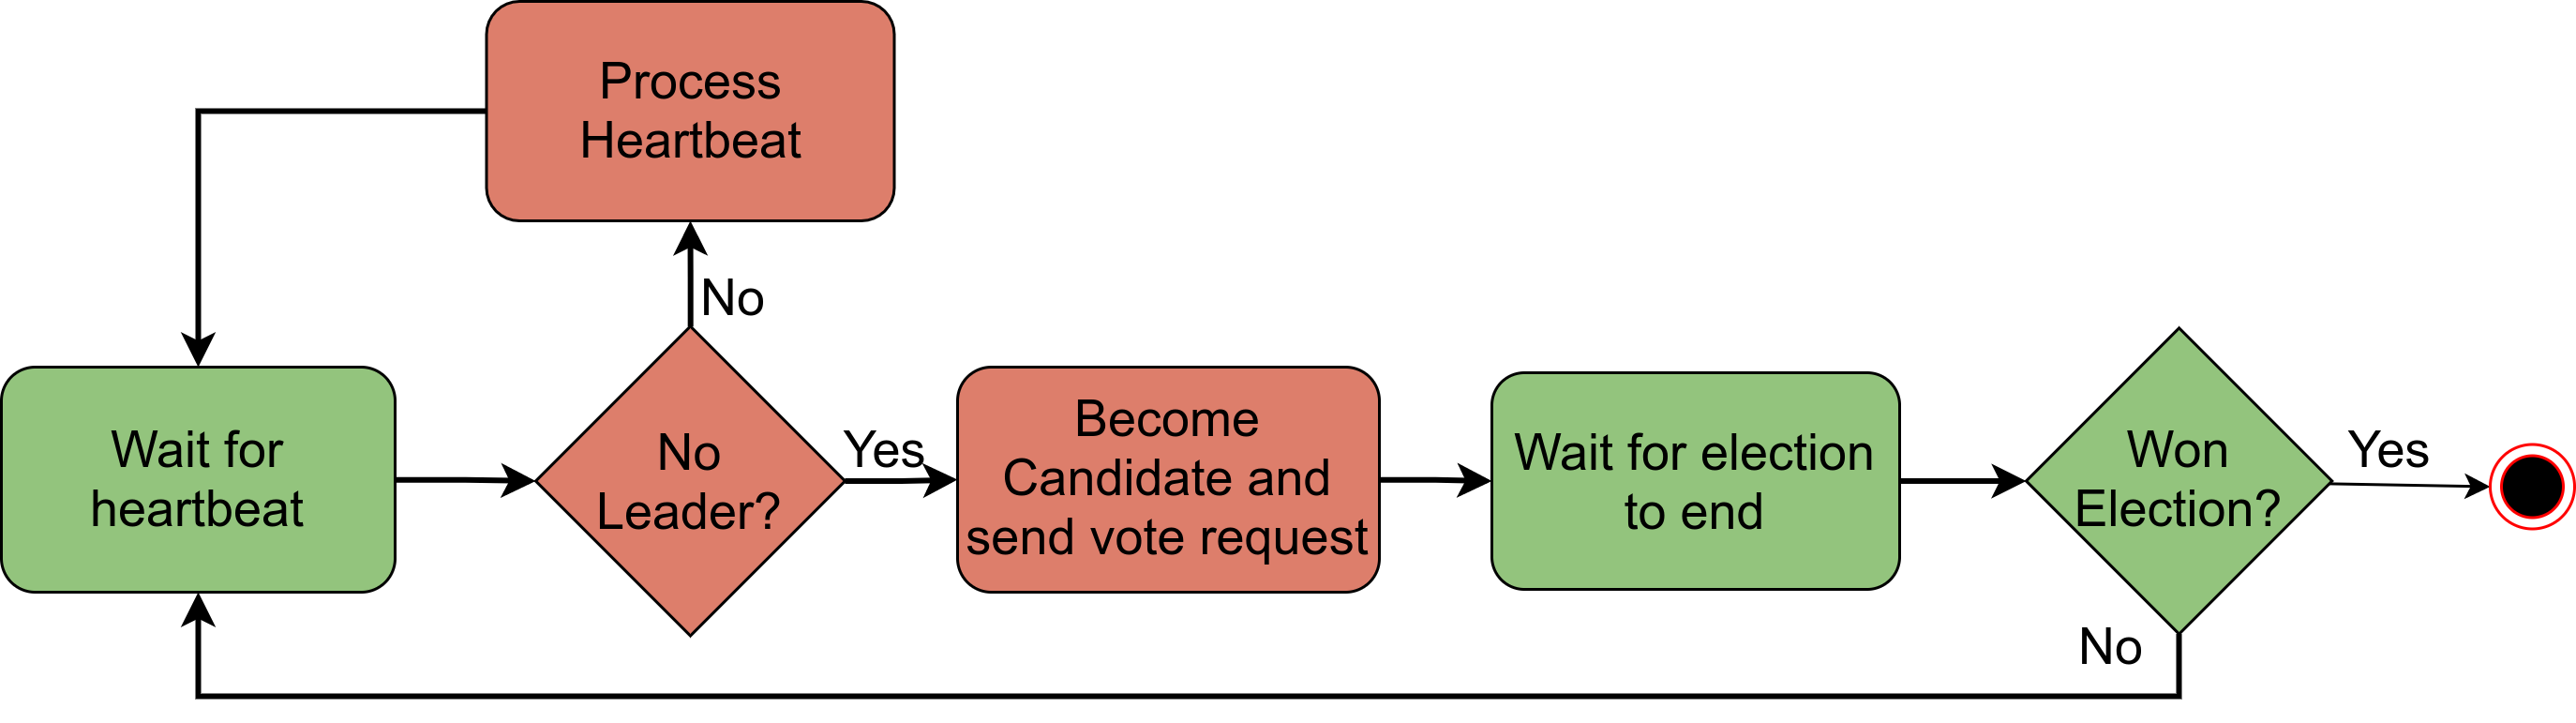
\includegraphics[width=0.9\linewidth]{images/LeaderElectionHeartbeatThread}
	\caption{One part of the leader election process is the monitoring of heartbeat messages. This task is performed by replicas that are in follower state and is used to identify a leader's absence. When no heartbeat messages are received for a certain period of time, a new leader election starts.}
	\label{fig:LeaderElectionHeartbeatThread}
\end{figure}

\begin{figure}[!hb]
	\centering
	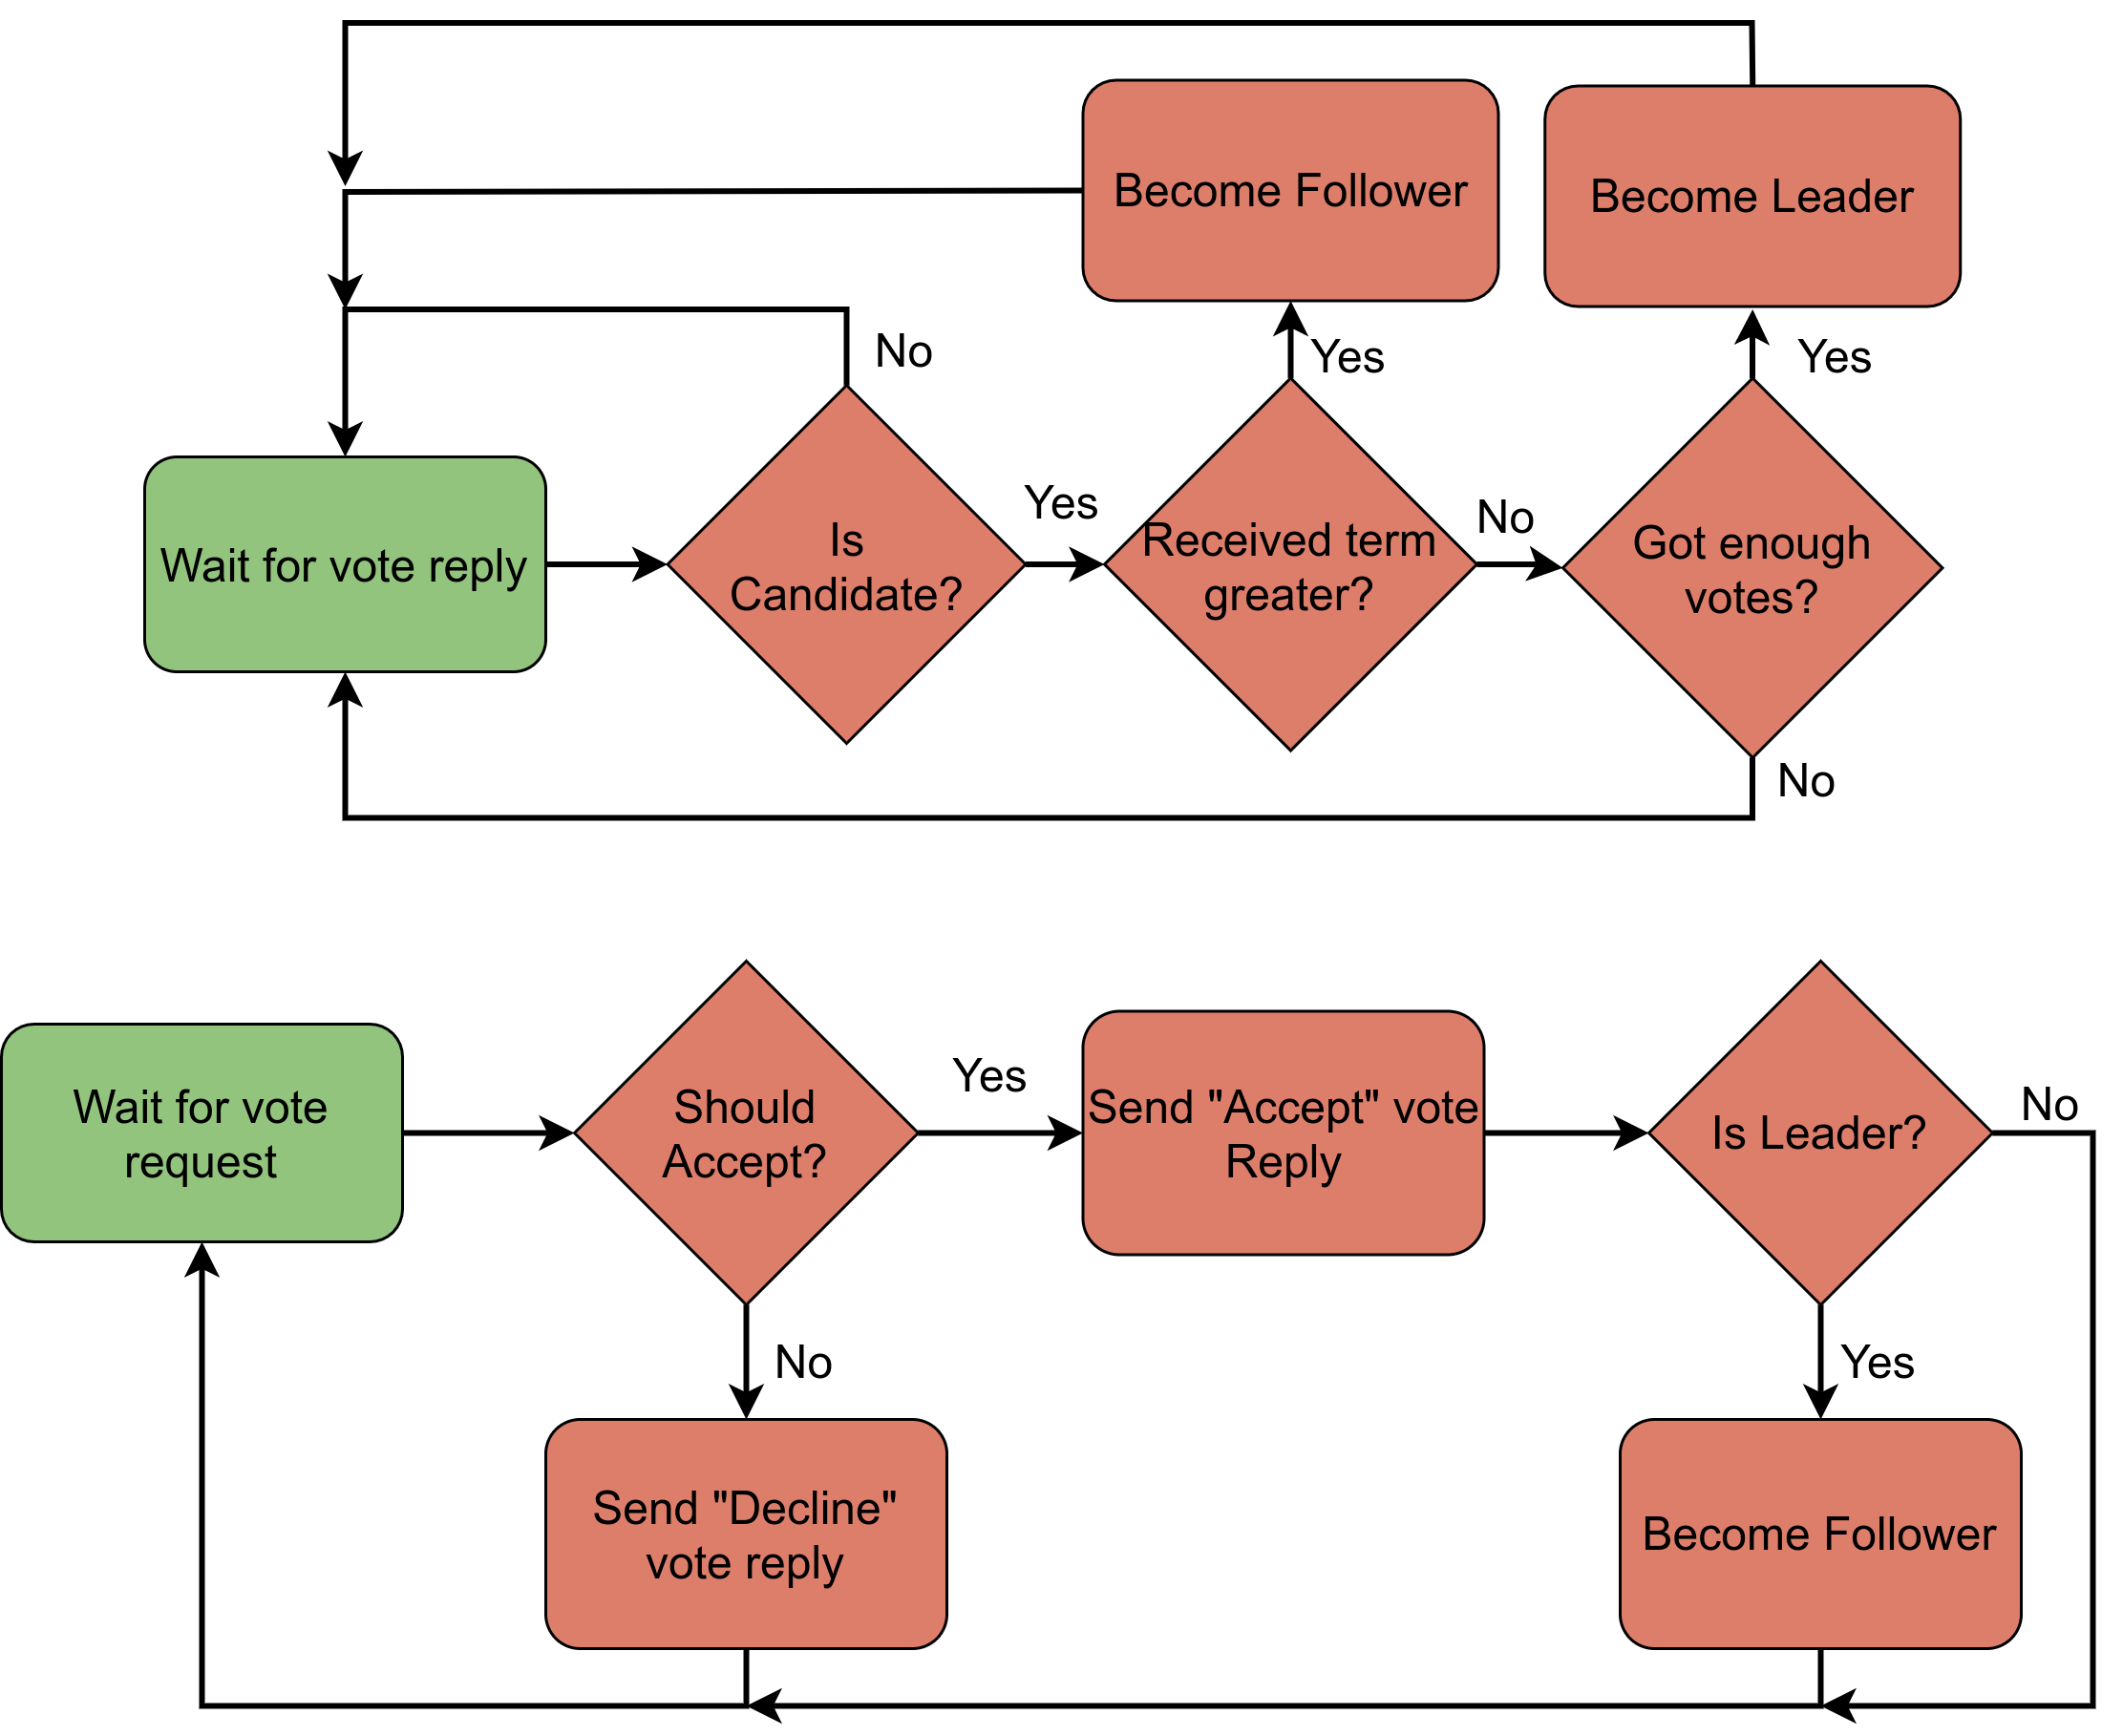
\includegraphics[width=0.9\linewidth]{images/LeaderElectionVoteThread}
	\caption{One part of the leader election process is making and answering vote requests. All replicas are permanently waiting for vote requests. Replicas in candidate state ask the other replicas for their votes and become the new leader after enough votes got accepted.}
	\label{fig:LeaderElectionVoteThread}
\end{figure}


The leader election algorithm is structured into three parts executed on two \abr{OS} threads.
One part is the processing of heartbeat messages in a \texttt{Heartbeat Thread}, as depicted in~\autoref{fig:LeaderElectionHeartbeatThread}.
In the \texttt{Heartbeat Thread}, a follower listens for heartbeat messages and starts a leader election process by sending vote requests when the corresponding timeout expires.
The other two parts, namely answering vote requests and processing replies to vote requests, are handled in another thread and are depicted in~\autoref{fig:LeaderElectionVoteThread}.
Replica-internal race conditions are prevented by utilizing a mutex in order to ensure that its private state - including the replica's \texttt{Raft} role, the current term, and voting information - does not change while answering a message.
Race conditions among replicas are prevented through a history \abr{QOS} policy and a continuously increasing term number.
The history \abr{QOS}-policy ensures that new requests are buffered in a \texttt{DataReader} while another is processed.
This ensures that no request is neglected.
Further, a continuously increasing term number enables the system to detect outdated requests or recognize when the replica itself is outdated.

\subsubsection{Timing Considerations}
\label{subsub:timeConsiderations}

Because each \texttt{WaitSet} in \abr{DDS} can be attached with a timeout, the maximal time that the system is without a leader can be determined.
This is further measured and analyzed in~\autoref{cpt:evaluation}.
There are two timeouts involved in the leader election process, namely the \textit{election timeout} - whereby a missing leader is detected - and the \textit{leader ready timeout}.
An expiring \textit{leader ready timeout} indicates that the system could not elect a new leader for the given term.
This can, for example, happen due to split votes when multiple followers try to become the new leader at the same time or because there are not enough active replicas in the system.
The proposal that \texttt{Raft} makes to reduce the risk of split votes is to use randomized \textit{election timeouts}.
However, this does not prevent split votes from happening at all.
Therefore, in this implementation, the \textit{election timeout} is made directly dependent on the replicas' unique identification number, so that they never try to become a leader at the same time.
Replicas with certain identification numbers are thereby preferred in the leader election process.
However, this approach is not a disadvantage because - due to \abr{DDS}'s global data space - no replica is ever more suitable for becoming the new leader than some other.
Further, a replica with an outdated term number is still excluded from becoming a leader because their vote requests would get declined.

The problem that not enough replicas are active for an election can be solved by specifying the maximum number of consecutive terms that an election is allowed to fail.
Since the \textit{leader ready timeout} states the maximum duration of a failed election, a maximal time that the system is allowed to be without a leader can be specified.
Any replica that recognizes that an election is impossible can then bring the train to a halt.
Altogether, when enough replicas are present in the system and communication is possible without any delays, the system will not be without a leader for the maximum time of $\textit{election timeout} + \textit{leader ready timeout}$.
\\

Whether a replica writes data onto a topic or reads data from a topic depends on its \texttt{Raft} role.
For example, the leader publishes heartbeat messages while a follower receives the heartbeat messages to detect a missing leader.
Because a replica can become the leader or a follower at any point in time, it cannot be predicted when it transitions from publisher to subscriber or from subscriber to publisher.
This can be a safety hazard because registering a publisher or subscriber can fail and it takes time to register an \abr{DDS} entity to a topic.
Therefore, every replica is set up to simultaneously act as a publisher and subscriber to every topic, with an exception to the \texttt{Input} topic.

However, this also means that each replica receives its own messages.
Therefore, after reading each data sample, the application code must manually verify that the message was not published by the same replica reading the message.
This is done by comparing the receiving replica's identification number with the received \textit{senderID}.
Even though this results in a consistent computational overhead, it increases the implementation's predictability and, thereby, its safety.

\subsection{Decision Making}
\label{subsec:ImpInputProcessing}

\begin{figure}[!hb]
	\centering
	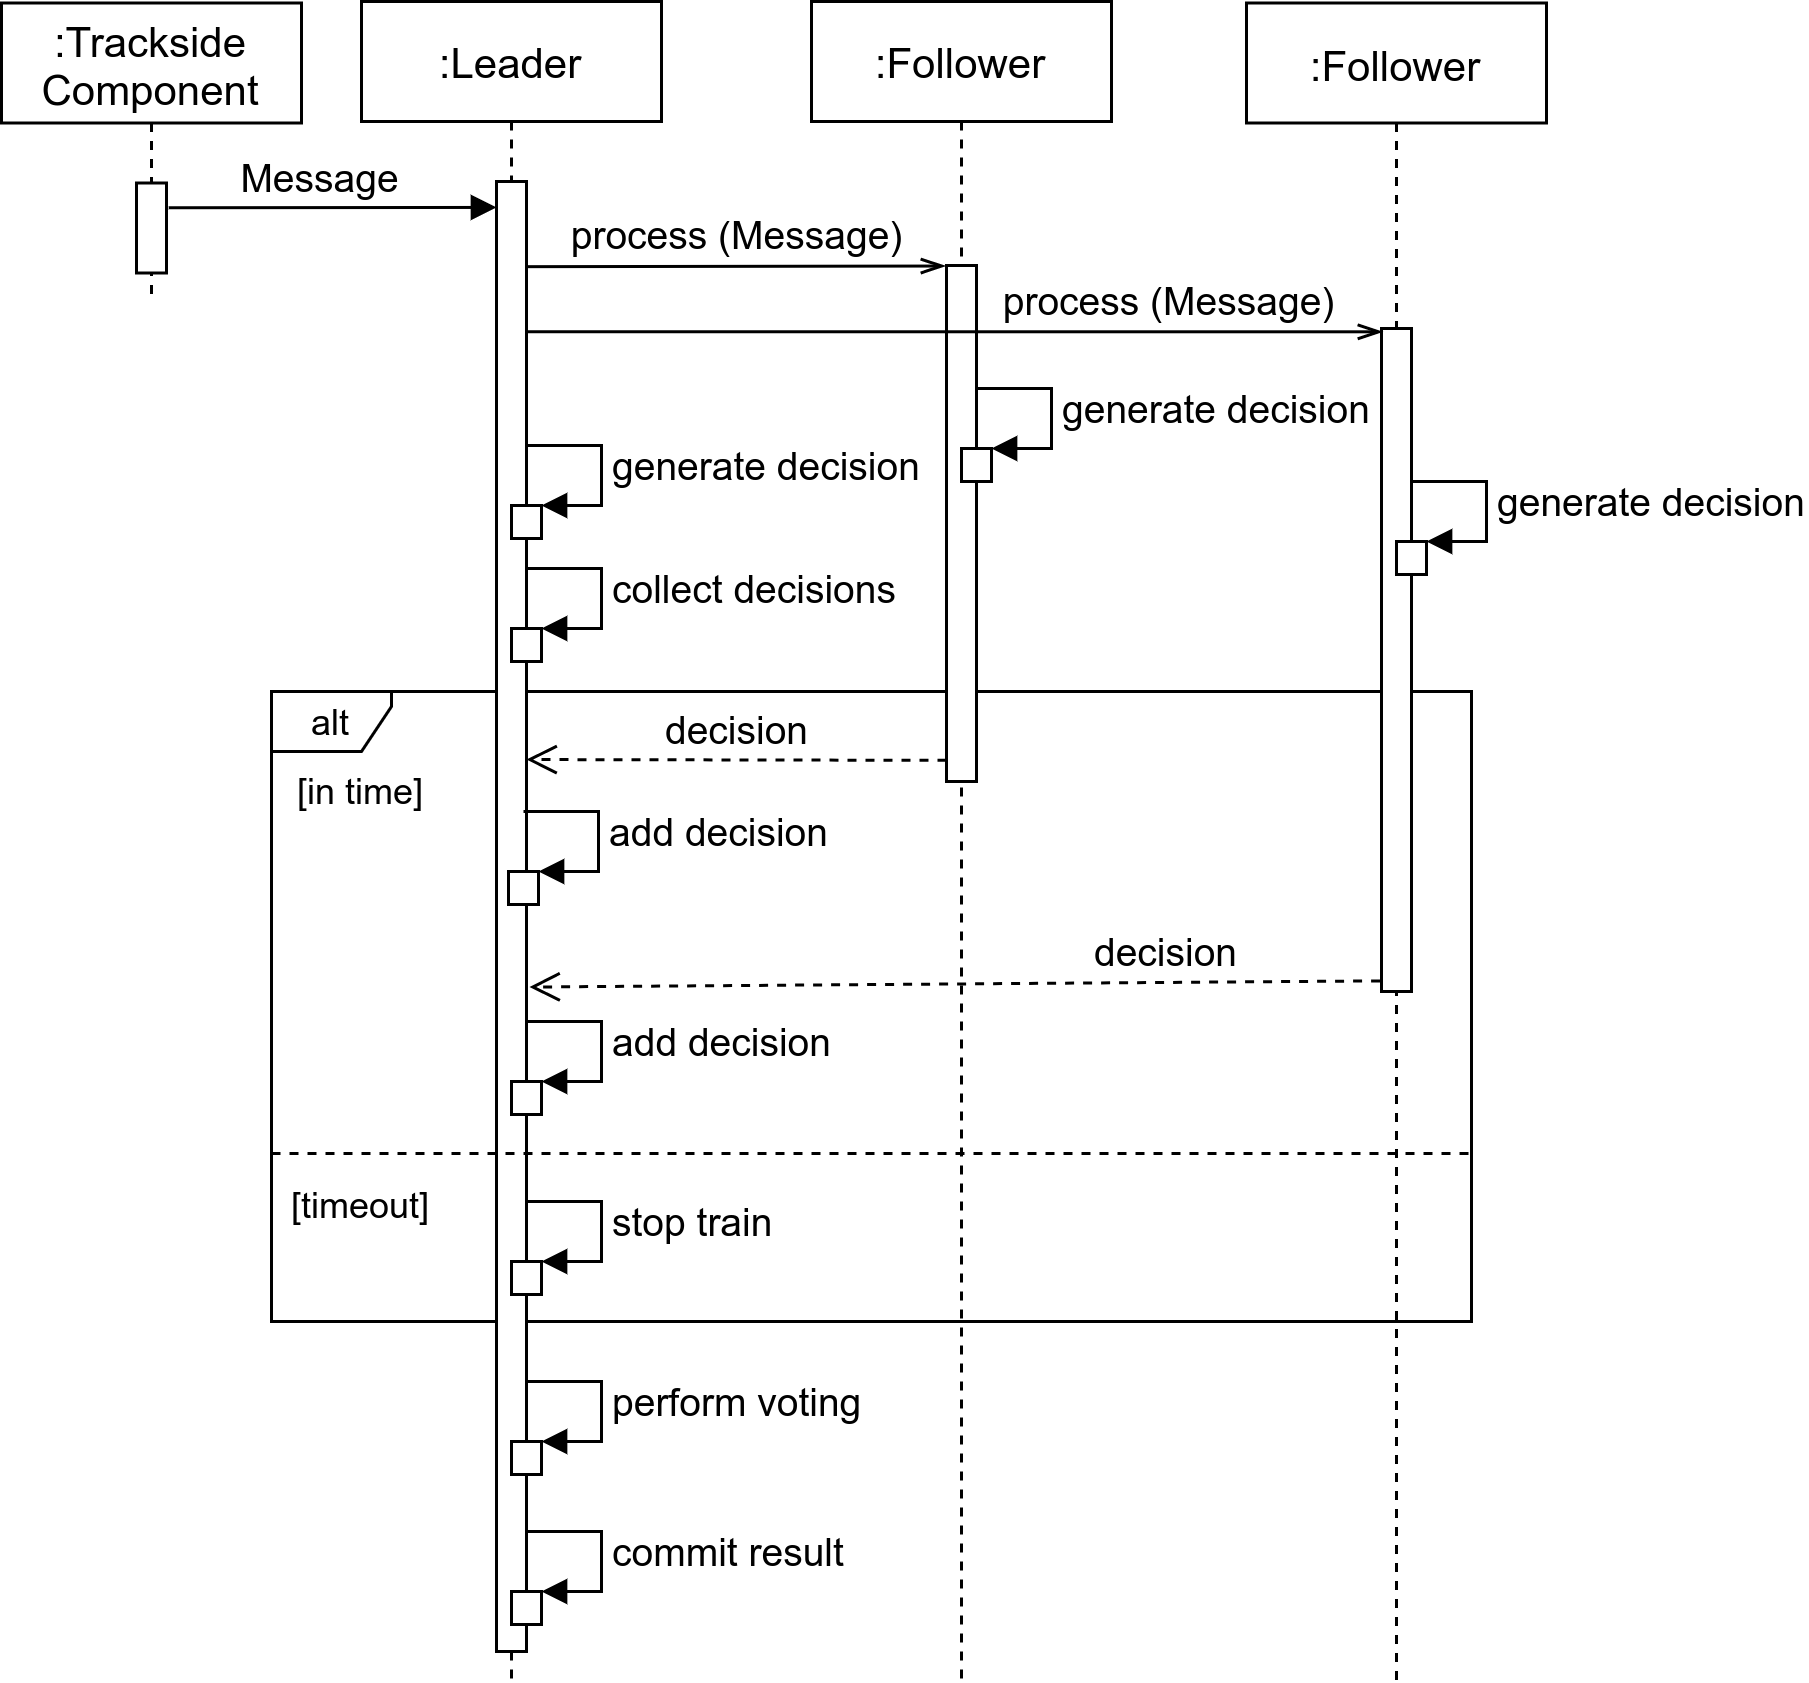
\includegraphics[width=0.8\linewidth]{images/sequence/CollectResults}
	\caption{The leader records input messages from track-side components. Afterward, the leader sends a message with an input reference to each follower in order to request a decision. Then, the leader and each follower process the input and generate a decision based on the input and the global system state. The decisions are collected by the leader that performs a voting when enough decisions are present. Meanwhile, the leader ensures that time constraints are met using timeouts. If there are not enough decisions for voting after the timeout expires, the train must be slowed down.}
	\label{fig:SeqCollectResults}
\end{figure}

Critical input messages, such as balise telegrams, require safety-critical computations and are therefore redundantly processed by the system.
Based on these redundant decisions, the system's leader generates a final system output by performing a majority voting.
A coarse overview of how the redundant computation and voting is performed is shown in~\autoref{fig:SeqCollectResults}.
\\

It is the leader's responsibility to record new inputs, request redundant decisions from the remaining replicas, and generate a voted output based on the redundant decisions.
Therefore, the leader sends a \textit{process} request and a reference to the corresponding input to each follower.
Upon receiving this request, the replicas start to generate a decision for the input.
After sending the request, the leader generates a decision itself and waits for the remaining replicas' decisions.
The leader can perform a majority voting when it received enough redundant decisions after a certain period of time called \textit{processing timeout}.
If there are too few decisions and the system's time constraints are violated, the train must be stopped.
\\

After the leader successfully performed a voting, it commits the final decision.
The commit phase consists of three steps.
First, the system's global state is altered based on the voted decision.
For example, when a linked balise's telegram has been processed, the confidence interval is adjusted to the balise's position.
Second, the leader outputs the voted decision as the system's output.
Third, the corresponding input is marked as processed on the \texttt{Input} topic by disposing of the corresponding \abr{DDS} instance.
This ensures that the next leader will read and process the input if the previous leader is deselected or crashed before committing a result.
\\

Communication between the leader and its followers happens via \abr{DDS} topics.
A \texttt{WaitSet}, attached with a \texttt{ReadCondition}, is used to recognize new messages on the \texttt{Input} topic.
As soon as the leader recognizes a new input message, it sends a \textit{process} request.
The \textit{process} request follows \texttt{Raft}'s log replication approach and is transmitted via the \texttt{AppendEntries} topic.
As soon as a follower receives the \textit{process} instruction, it starts to generate a decision for the referenced input and publish the decision to the \texttt{AppendEntriesReply} topic.
Simultaneously, the leader also generates a decision and waits for follower responses on the \texttt{AppendEntriesReply} topic using a \texttt{WaitSet} and a \texttt{ReadCondition}.

\subsubsection{Safety Considerations}

In order to ensure the train's integrity, every replica's default decision is to brake.
When a balise telegram is received, the train is only allowed to continue its journey if all of the following conditions are met:

\begin{enumerate}
\item The train is currently driving.
\item The balise, to which the received telegram belongs, has been linked.
\item According to the linking information, the balise telegram has been received at the position where the balise should be.
\item According to the braking curve, the train would not reach the current \abr{MA}'s end.
\end{enumerate}

Further, the train's braking curve needs to be periodically monitored independently of incoming balise telegrams.
Therefore, a timeout is attached to the \texttt{Input} topic's \texttt{WaitSet} that expires when no input message is received for a specific period.
Upon expiring, the leader behaves as if an input message has been received.
First, the leader requests redundant decisions whether the train should brake or continue its journey.
Second, the leader calculates a decision itself by calculating the braking curve and comparing it to the current \abr{MA}'s end position.
Third, it waits for results from the remaining replicas and performs a majority voting.
Finally, the voted result is send as a system output.

In the following, both monitoring the braking curve and handling critical inputs is referred to as \textit{input processing}.
\\

When the leader crashed during the small time frame between serving the voted decision as the system's output and marking the corresponding input as processed, an input could be processed twice.
However, it is assumed to be very unlikely that such a situation happens.
In an alternative situation, when the leader would not mark the input as processed, the leader might crash while processing the input, and the input would not be processed at all.
The probability that the leader crashed while processing the input is higher than the probability that it would crash between serving the output and marking the input as processed.
Therefore, the risk of a single input being processed twice is accepted because the alternative is worse and more likely.
\\

For the replicas to generate deterministic and relevant decisions, every replica requires access to the system's most recent global state.
Thus, \abr{DDS} is utilized to manage the system's global state in state topics.
The \texttt{State Manager} component, that is responsible for managing the global state, is described in~\autoref{sec:stateManager}.

Because only the leader can change the global state, updates must be sent to all replicas.
Hence, redundant decisions can be based on different state information and thereby affect the system's safety.
A possible way to reduce the chance of such situations, input processings should be repeated when the leader's decision was outnumbered in the voting.
However, only if the repetition would not jeopardize any time constraints.

\subsubsection{Timing Considerations}

After the leader sent a decision request to every other replica and generated a decision itself, it waits for responses to continue with voting.
Since the system consists of independent replicas, it is impossible to predict how long it will take the other replicas to generate a decision.
In order to prevent the voting process from being deferred indefinitely, a timeout is attached to the \texttt{WaitSet} for the \texttt{AppendEntriesReply} topic.
Consequently, two situations are possible while the leader waits for responses on the \texttt{AppendEntriesReply} topic.
First, the leader receives a response from every replica before the timeout expires.
Second, the timeout expires before a response from every replica has been received.
In the first situation, voting is possible without any problems.
In the second scenario, the leader can only continue when a response from more than half of the replicas in the system have been received.
If the leader received an even number of decisions, split votes in the voting process are possible.
In case of split votes, the most restrictive one has to be chosen.
Receiving too few decisions is a safety risk and the leader must stop the train.
\\

In addition, a leader could repeatedly crash while processing an input.
Thereby, the system would not be able to generate an output for a critical input.
he presented system cannot cope with such a situation because it would require a distributed timeout that is not possible for an asynchronous system~\cite{FLPProblemConsensus}.
It could be solved by an external instance that recognizes incoming inputs and stops the train when it is not notified that an output has been generated.
In practice, the antenna unit could perform this task by applying a counter and being connected to the on-board unit's output line.

\section{System Recovery}

The failure of system components reduces the system's reliability (ref.~\autoref{sec:techniquesSafetyReliability}).
This section describes methods by which the system can recover from the failure of individual components and thus retain its reliability.
Such procedures are based on the concepts of error detection, location, and recovery.
\\

First, the implementation of hot standby redundancy using DDS concepts is described.
Afterward, it is explained how the hardware watchdog of the \textit{Revolutions Pis} can be used to increase reliability - as proposed by Sakic and Kellerer~\cite{SakicTimeInConsensus}.

\subsection{Hot Standby}
\label{sec:HotStandby}

\begin{figure}[!ht]
	\centering
	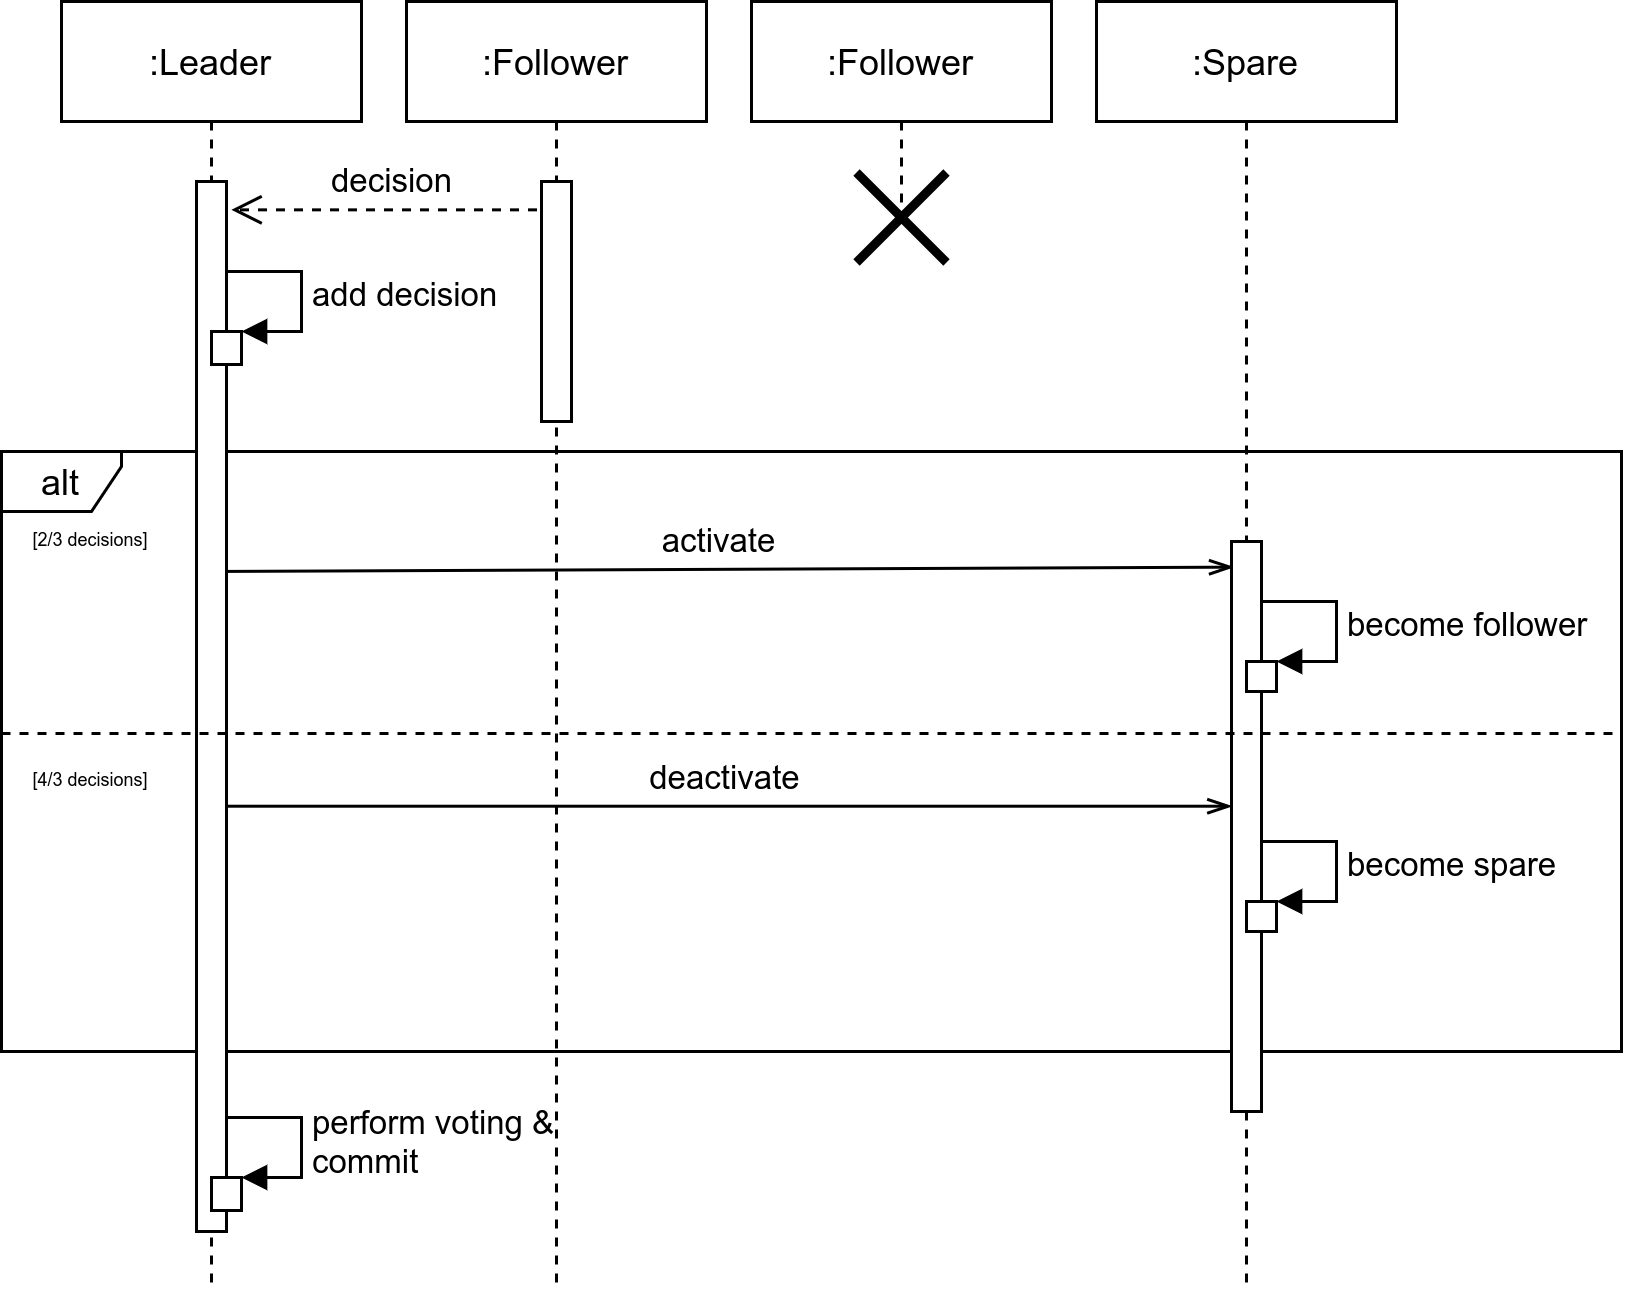
\includegraphics[width=0.75\linewidth]{images/sequence/ActivateSpare}
	\caption{When the leader, after reading an input message and instructing its followers to process the input, receives too few decisions after a certain time, it activates the spare replica. When the follower receives more than necessary, the spare component gets deactivated again.}
	\label{fig:SeqActivateSpare}
\end{figure}

Active hardware redundancy facilitates systems to recover from individual component failures.
An algorithm for adding a spare component as a hot standby is depicted in~\autoref{fig:TMRWithSparesDDS}.
If the leader receives too few decisions when processing an input, it assumes that any non-responsive replica has crashed.
Thereupon, the leader activates the spare by publishing a message to a \abr{DDS} event topic called \texttt{ActivateSpare}.
If the replica has was assumed to be crashed responds again, the spare can be deactivated again by publishing a corresponding message to the \texttt{ActivateSpare} topic.
\\

For creating a hot standby, a component must be initialized in spare mode.
Spare mode implies that the component is initialized as any other component but additionally subscribes to the \texttt{ActivateSpare} topic.
Further, a spare utilizes a \texttt{WaitSet} to wait for any activate message.
\\

Unlike the other replicas, a spare component can only be in \texttt{spare} or \texttt{follower} mode and is excluded from becoming the leader, as well as from voting for other leaders in the leader election process.
This is because a spare component can be activated or deactivated at any time.
Upon being activated, a spare component participates in the input processing process by responding to leader requests.
\\

Although only a single spare component is currently supported, multiple spares can be added by introducing a \texttt{spareID} field to \texttt{ActivateSpare}.

\subsection{Watchdog}

A watchdog is an important safety feature and proposed by Sakic and Kellerer~\cite{SakicTimeInConsensus} to increase a system's probability to respond when a component failed.
The \textit{Revolution Pi Connects} install a configurable hardware watchdog in the form of a watchdog timer on a dedicated hardware chip.
The timer must be manually and periodically reset.
When it is not reset, the timer expires and the corresponding \abr{PLC} gets restarted.
This allows the watchdog to restart a replica when the on-board unit software stops responding.
\\

In order to take advantage of the hardware watchdog, the heartbeat mechanism used for the consensus algorithm is exploited.
Each time the leader sends a heartbeat, it also resets the watchdog timer.
For followers, the watchdog timer is reset upon receiving a heartbeat message.

On the one hand, this increases the system's reliability because certain exceptions and faults such as memory corruptions that result in a stopped software can be repaired by restarting the system.
On the other hand, an appropriate watchdog timeout must be small enough to restart a faulty component as soon as possible but long enough not to trigger false positives.
Since resetting the timer is bound to the heartbeat mechanisms, the maximum time that the system can be without a leader needs to be known.
This is analyzed in~\autoref{subsec:LeaderElectionEval} and marks the watchdog timer's lower limit.











\iffalse






\begin{figure}[!hb]
	\centering
	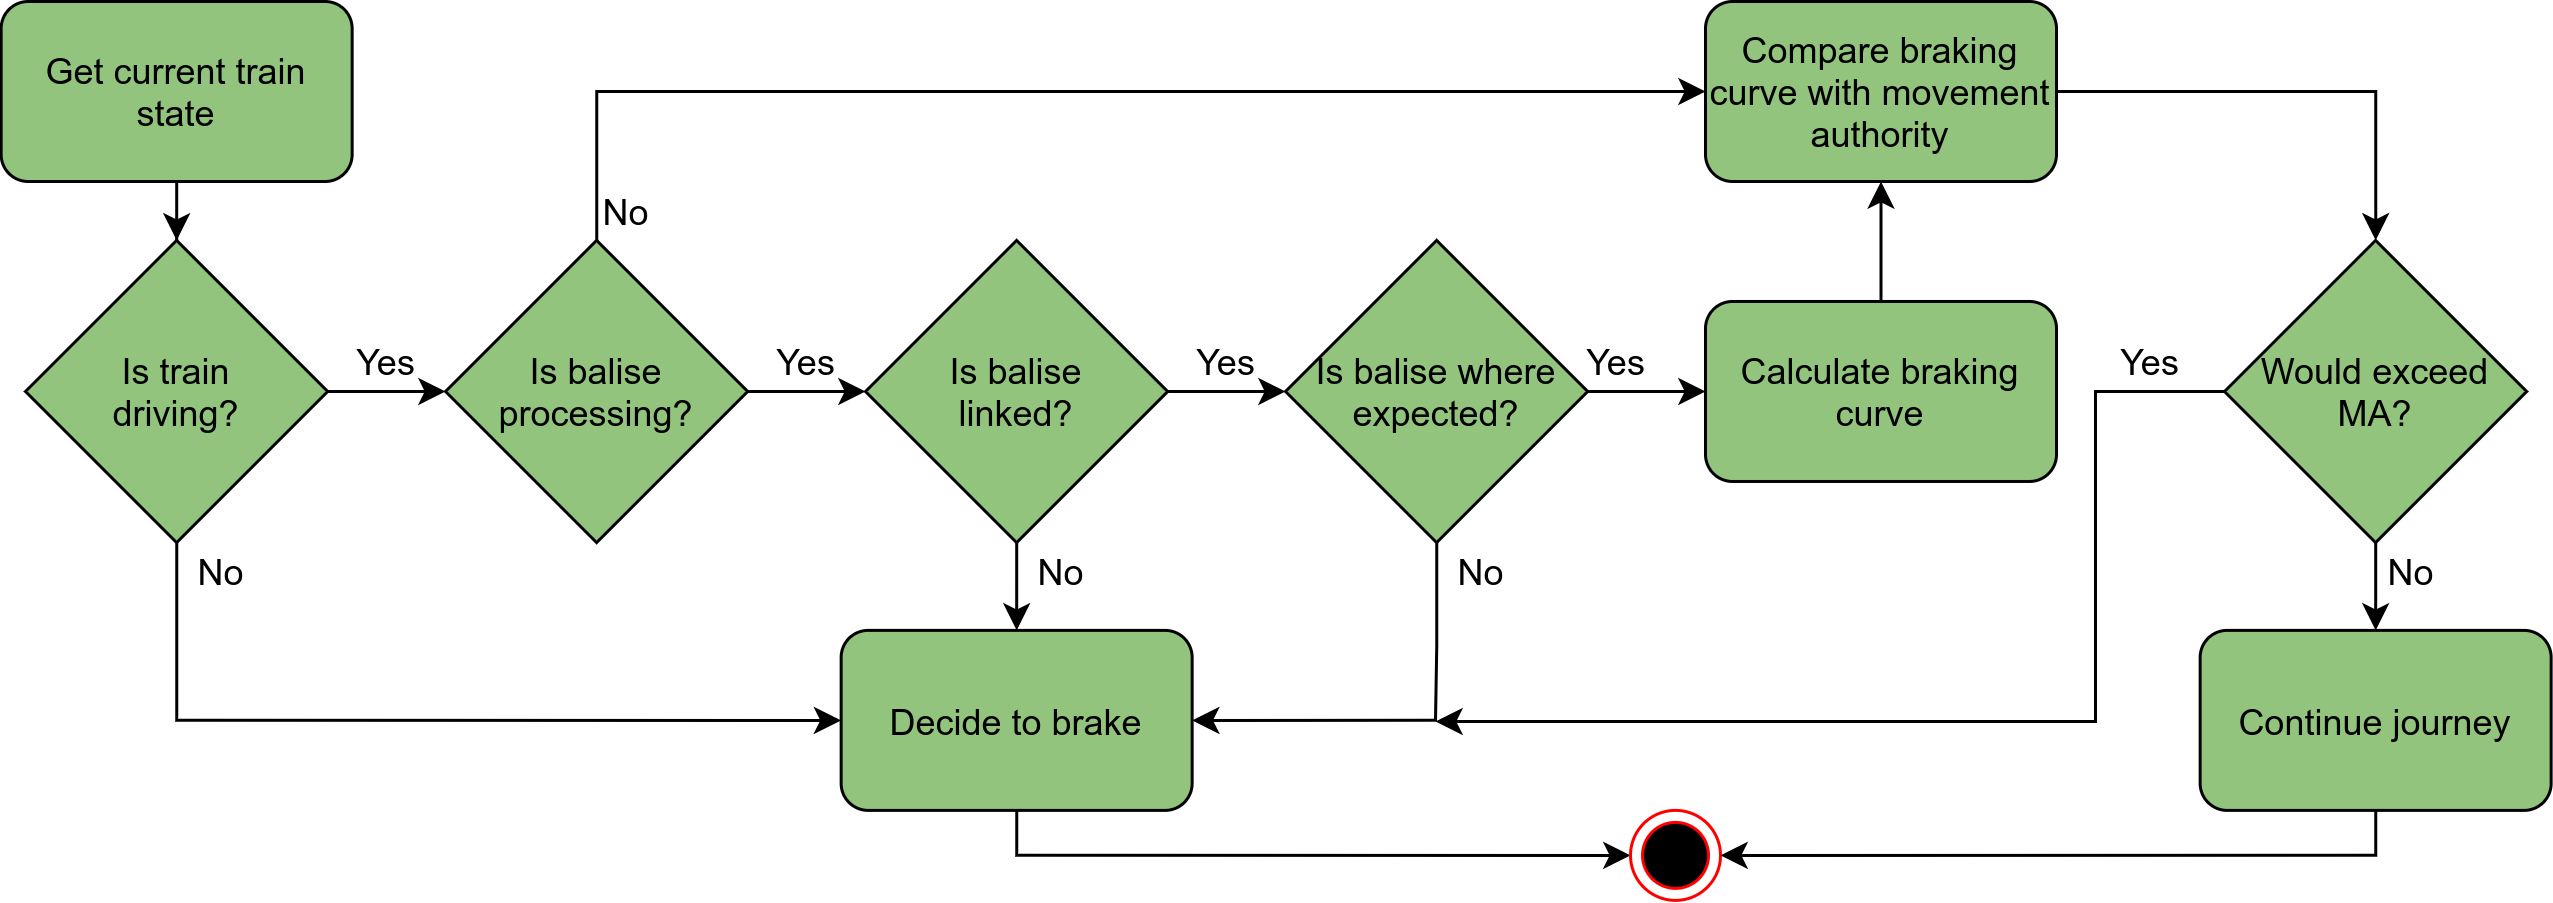
\includegraphics[width=0.75\linewidth]{images/DecisionMaking}
	\caption{To decide whether the train should brake or can continue its journey, this algorithm is executed. When the train is not driving, it should brake. IF a balise telegram is evaluated, it is checked whether the balise is linked and whether the calculated train position corresponds with the balise's expected position. Finally, the train's braking curve is calculated and it is checked, whether the train would reach the current \glsentryfull{MA}'s end position when it would brake in this moment. Only if everything goes as planned may the train continue its journey.}
	\label{fig:DecisionMaking}
\end{figure}

\begin{algorithm}[H]\caption{TODO.}\label{algo:DecisionMaking}
\SetKwData{MA}{\textit{\abr{MA}}}
\SetKwData{LinkedBalises}{\textit{linked balises}}
\SetKwData{TrainState}{\textit{train state}}
\SetKwInOut{Input}{input}
\SetKwInOut{Output}{output}

\Input{A balise telegram to process, the current \MA, the set of \LinkedBalises, and the \TrainState}
\Output{Decision to brake or continue the journey}
\BlankLine

\If{The train is not driving}{
brake\;
return\;
}
\If{processed balise is not linked}{
brake\;
return\;
}
\If{processed balise's position not in confidence interval}{
brake\;
return\;
}
calculateBrakingCurve()\;
\If{Train would reach end of \MA when braking now}{
brake\;
return\;
}
continue journey\;
return\;
\end{algorithm}





\lstset{language=C}
\begin{lstlisting}[caption={\abr{IDL} definition for the \texttt{AppendEntries} topic. The \texttt{term} variable represents the latest term that the replica has seen, while the \texttt{senderID} encodes which replica sent this message. With \texttt{entries}, a payload can be send via the topic. This is used by a leader for instructing its followers to process certain data. The \texttt{entries} field is left empty for heartbeat messages.}, label=code:appendEntries]
struct AppendEntries {
    long term;
    long senderID;
    sequence<Entry> entries;
};
#pragma keylist AppendEntries term
\end{lstlisting}

\begin{lstlisting}[caption={\abr{IDL} definition for the \texttt{RequestVote} topic. The \texttt{term} variable represents the candidate's term, while \texttt{candidateID} encodes the candidate that requested the vote.}, label=code:requestVote]
struct RequestVote {
    long term;
    long candidateID;
};
#pragma keylist RequestVote
\end{lstlisting}

\begin{lstlisting}[caption={\abr{IDL} definition for the \texttt{RequestVoteReply} topic. The \texttt{term} encodes the sender's term for the candidate to update itself. \texttt{voteGranted} shows whether the replica granted the vote request for the given term. The \texttt{candidateID} and \texttt{senderID} are used to identify which replica granted the vote for which replica respectively.}, label=code:requestVoteReply]
struct RequestVoteReply {
    long senderID;
    long term;
    long candidateID;
    long voteGranted;
};
#pragma keylist RequestVoteReply
\end{lstlisting}



\begin{lstlisting}[caption={\abr{IDL} definition for the \texttt{LinkedBalises} topic. Each linked balise has an unique identifier and a position that is communicated to the system by the \abr{RBC}.}, label=code:linkedBalises]
struct LinkedBalises {
    short ID;
    long position;
};
#pragma keylist LinkedBalises ID
\end{lstlisting}

\begin{lstlisting}[caption={\abr{IDL} definition for the \texttt{MovementAuthority} topic. The \texttt{start\_position} encodes where the \abr{MA} starts and the \texttt{end\_position} encodes until where it is valid.}, label=code:movementAuthority]
struct MovementAuthority {
    long start_position;
    long end_position;
};
#pragma keylist MovementAuthority
\end{lstlisting}

\begin{lstlisting}[caption={\abr{IDL} definition for the \texttt{TrainState} topic. The train's state consists of a current position and a current speed. Due to inaccuracies of the position sensors, a train's position cannot be determined exactly. Therefore, a confidence interval is maintained that defines an area where the train certainly is. This area is bounded by \texttt{max\_position} and \texttt{min\_position}. With \texttt{is\_driving} it is encoded whether the virtual train drives or stands still. The \texttt{lastUpdateTime} variable is used to simulate the train's position based on its speed.}, label=code:trainState]
struct TrainState {
    double position;
    double max_position;
    double min_position;
    double speed;
    boolean is_driving;
    unsigned long long lastUpdateTime;
};
#pragma keylist TrainState
\end{lstlisting}

\begin{lstlisting}[caption={\abr{IDL} definition for the \texttt{ActivateSpare} topic. This topic is used to activate or deactivate spare replicas. The \texttt{term} field encodes the term in which the activate or deactivate call has been made and \texttt{activate} gets interpreted as a boolean that encodes whether the spare should be activated or deactivated.}, label=code:activateSpare]
struct ActivateSpare {
    long term;
    long activate;
};
#pragma keylist ActivateSpare
\end{lstlisting}

\fi

    \chapter{Evaluation}
\label{cpt:evaluation}
In this chapter, the developed system is evaluated with respect to various criteria.
At first, an overview about the utilized \abr{DDS} subset is described and the necessity of each feature is justified.

This is followed by an system evaluation where both the system's hardware structure as well as the implemented software are evaluated.
Within the implementation evaluation, all characteristics that correspond with the manner of how the software is implemented, are considered.
First, general system properties are analyzed, such as the time needed to send and receive messages or the maximum time the system can be without a leader.
This allows to answer fundamental questions about the system's reliability because the average time to synchronize the components can be derived.
Afterwards, metrics related to the execution of specific scenarios are examined.
These include the utilization of system resources on the one hand and the number of messages sent and received on the other.
From these metrics it can be seen at which points in time an increase in system performance can be expected and that enough resources are always available in the applied system.

\section{DDS Subset Identification}

For reducing costs incurred in the system approving process, it is important to limit the amount of utilized features and lines of code.
Therefore, a subset of \abr{DDS} features from OpenSplice DDS, that is sufficient for building a redundant system, is identified.
An overview about this subset is given and justified in the following.
This overview only contains the methods and functionalities that are directly used by the application, the middleware, however, might utilize other functionalities to implement the features mentioned in this section.

\paragraph{Domain Module}
A \abr{DDS} application's main building blocks comprise a \texttt{Domain}, one or multiple \texttt{DomainParticipants}, as well as a \texttt{DomainParticipantFactory} for creating new \texttt{DomainParticipants}~\cite{omgDDSspec}.
Besides these classes, the domain module contains various functionalities, from which only the following subset is used within the exemplary implementation.

\begin{itemize}
\item \textit{DDS\_Entity\_get\_instance\_handle} Is used for acquiring an instance handle to mark it as processed in the leader's commit phase.
\item \textit{DDS\_DomainParticipant\_create\_(publisher|subscriber|topic)} Is used for creating \abr{DDS} publishers, subscribers or topics.
\item \textit{DDS\_DomainParticipant\_delete\_(publisher|subscriber|topic)} Is used for deleting \abr{DDS} publishers, subscribers or topics.
\item \textit{DDS\_DomainParticipantFactory\_get\_instance} Used for acquiring the \texttt{DomainParticipantFactory} singleton.
\item \textit{DDS\_DomainParticipantFactory\_(create|delete)\_participant} Used for creating a new participant in the \abr{DDS} domain.
\end{itemize}

Even though \textit{DDS\_DomainParticipant\_get\_default\_(publisher|subscriber|topic)\_qos} is used in the implementation, it is not mandatory because one could set the default \abr{QOS} settings directly on the corresponding entity.

\paragraph{Topic-Definition Module}
The topic definition module contains everything related to topics.
The exemplary implementation utilizes \texttt{Topics}, for describing data in the application, and \texttt{TypeSupport} which describes a data type that is bound to a \texttt{Topic}.
Apart from these two classes, the following methods are used:

\begin{itemize}
\item \textit{DDS\_TypeSupport\_\_alloc} Used for creating a new \texttt{TypeSupport}.
\item \textit{DDS\_TypeSupport\_get\_type\_name} Used for getting a data type's default name, which is required to register it later on.
\item \textit{DDS\_TypeSupport\_register\_type} Used for registering a new data type name on a \texttt{DomainParticipant}.
\end{itemize}


\paragraph{Publication Module}
\texttt{Publishers}, as well as \texttt{DataWriters}, which are used for data distribution, are located within the publication module.
Besides these two classes, the following functionality is required for the exemplary implementation:

\begin{itemize}
\item \textit{DDS\_Publisher\_(create|delete)\_datawriter} Used for creating, respectively deleting, \texttt{DataWriter} objects.
\item \textit{DDS\_DataWriter\_write} Used for writing new data to an instance on a \abr{DDS} topic.
\item \textit{DDS\_DataWriter\_dispose} Used for marking processed inputs for deletion so that they are not processed twice.
\end{itemize}

\textit{DDS\_Publisher\_copy\_from\_topic\_qos} and \textit{DDS\_Publisher\_get\_default\_datawriter\_qos} are not necessarily required due to the same reasons stated above.

\paragraph{Subscription Module}
The subscription module resembles the publication module, but for reading and receiving data.
However, besides \texttt{Subscribers} and \texttt{DataReaders}, it also contains \texttt{DataSample}, \texttt{SampleInfo}, \texttt{ReadCondition}, and \texttt{QueryCondition}, which are utilized in the exemplary implementation.
\texttt{Subscribers} and \texttt{DataReaders} are required for receiving data, which is represented by a \texttt{DataSample}.
The \texttt{SampleInfo} data structure contains additional information for each \texttt{DataSample}, such as its instance handle or state, which makes it mandatory for the implementation as well.
\texttt{ReadConditions} are used in combination with \texttt{WaitSets}, so that the application can react to certain middleware states.
\texttt{QueryConditions} are extensions for \texttt{ReadConditions} that allow to filter the data samples that are covered by a \texttt{ReadCondition}.
All filter operations could be implemented directly in the application code, which would make \texttt{QueryConditions} redundant.

Further, the following functionalities from the subscription module were used:

\begin{itemize}
\item \textit{DDS\_Subscriber\_(create|delete)\_datareader} Used for creating, respectively deleting, \texttt{DataReaders}.
\item \textit{DDS\_DataReader\_(create|delete)\_readcondition} Used for creating, respectively deleting, \texttt{ReadConditions}.
\item \textit{DDS\_DataReader\_create\_querycondition} Used for creating \texttt{QueryConditions}.
\item \textit{DDS\_DataReader\_take\_w\_condition} Used for reading and removing data from a \texttt{DataReader}, filtered by a \texttt{ReadCondition}.
\item \textit{DDS\_DataReader\_return\_loan} Required for indicating the middleware that the application finished accessing a sequence of data. This allows the middleware to work with the data again.
\end{itemize}

\paragraph{Infrastructure Module}
The classes that are used from the infrastructure module include \texttt{QosPolicy} and \texttt{WaitSet}.
The \texttt{QosPolicy} class implements \abr{DDS}'s \abr{QOS} functionalities and is therefore mandatory for the system's correctness.
\texttt{WaitSets} are applied for ensuring the application's compliance with its time restrictions, because they allow the assignment of timeouts.
In addition to that, the following functionalities from the infrastructure module are applied:

\begin{itemize}
\item \textit{DDS\_WaitSet\_\_alloc} Used for creating new \texttt{WaitSets}.
\item \textit{DDS\_WaitSet\_attach\_condition} Used to attach a condition to the corresponding \texttt{WaitSet}.
\item \textit{DDS\_WaitSet\_detach\_condition} Used to detach a condition from the corresponding \texttt{WaitSet}.
\item \textit{DDS\_WaitSet\_wait} Stops the according thread until at least one of the attached conditions evaluates to true.
\end{itemize}

Further, the following \abr{QOS} are applied in the application:
\todo{Add after deciding}


\section{System Evaluation}
At first in this section, general system metrics are analyzed.
Afterwards, metrics related to concrete, simulated scenarios are considered.
For this purpose, three scenarios are processed one after the other by the redundant system and certain data are collected during this process.

\subsection{General System Characteristics}
General system properties include those that are independent of environmental influences.
This includes the time it takes the system to elect a new leader, from which the maximum time that the system without a leader can be derived.
The election time is limited by the replica's computational resources and by the speed of data transmission.
The latter is investigated in the next step by publishing and reading messages of different sizes through \abr{DDS} topics.
Finally, the resource utilization of the system in idle mode is examined.
Idle means that the train is at a standstill and the system is ready to start the journey.

\paragraph{Leader Election Time}
\todo{Redo measurements}
\begin{figure}[!hb]
	\centering
	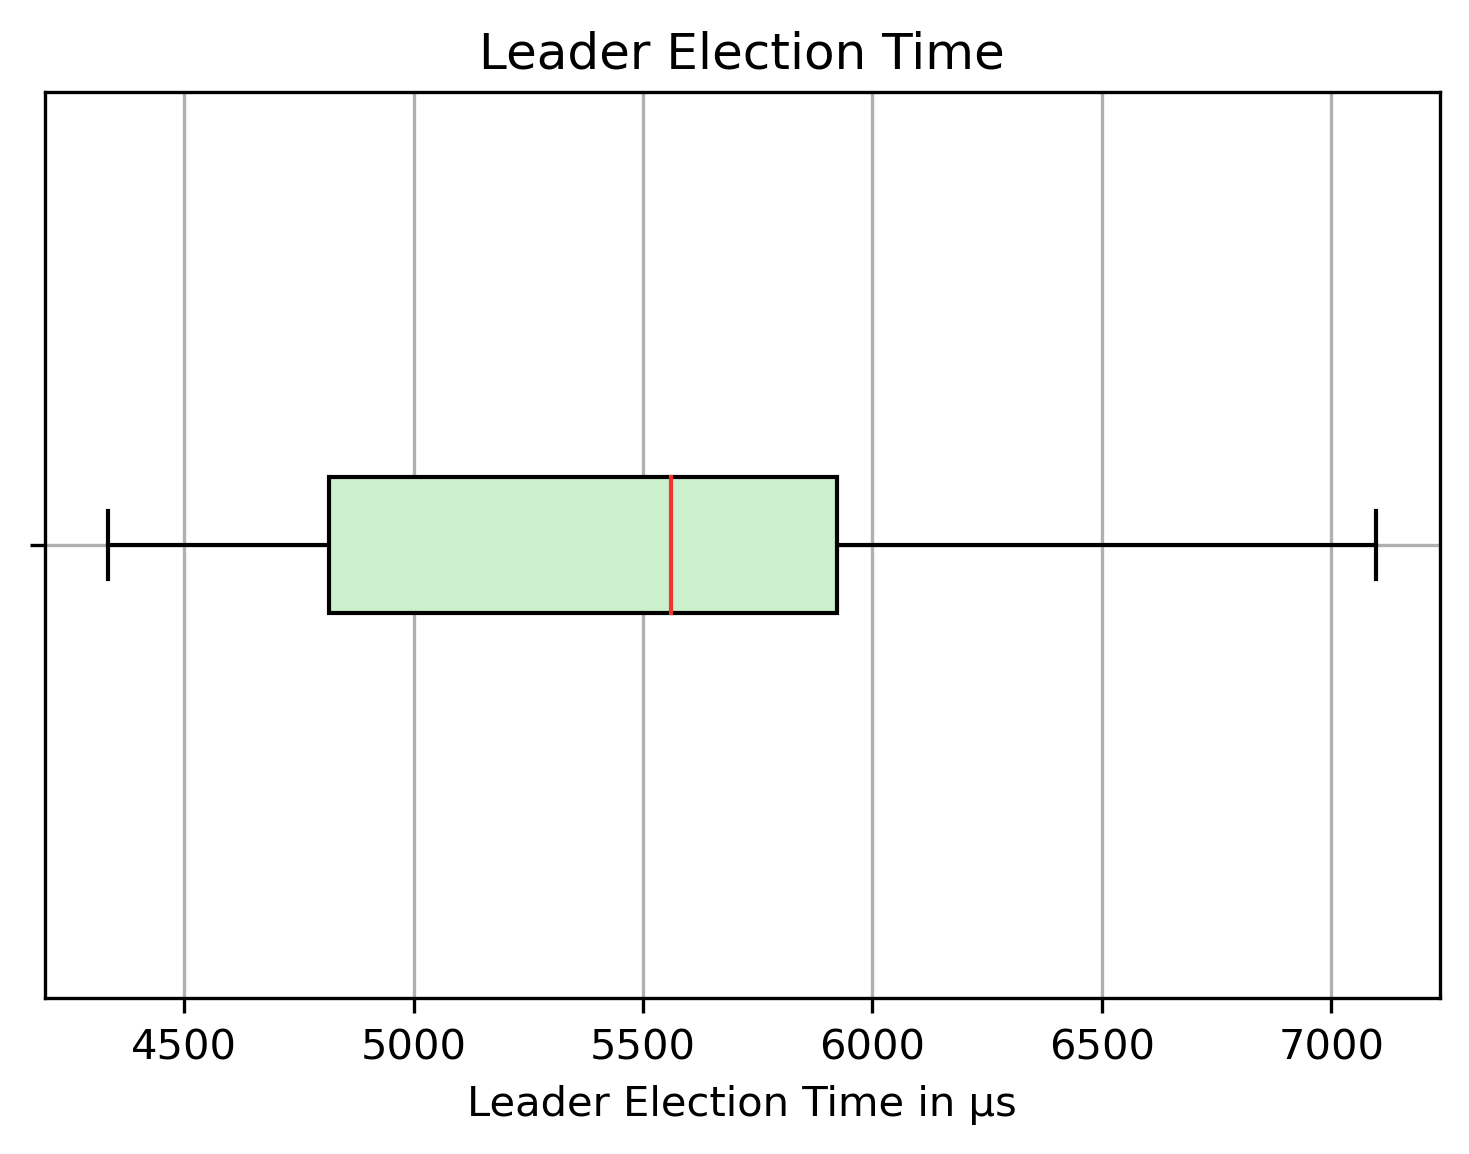
\includegraphics[width=0.75\linewidth]{images/plots/timeWithoutLeader}
	\caption{Time that the system is without a leader in each term for 20 terms. The average of 5472µs is marked by the red line.}
	\label{fig:PlotTimeWithoutLeader}
\end{figure}

When the system's leader crashes, the current \texttt{Raft} term ends and a new leader gets elected.
The leader election process consists of requesting and collecting votes from all replicas in the system.
In order to investigate how long the leader election process takes, the time for 20 elections was measured.
This has been done by starting a timer when a missing leader got noticed until a heartbeat message from a new leader was received.
The results can be seen in~\autoref{fig:PlotTimeWithoutLeader} and show that the process takes around 5500µs on average and at worst 7000µs.
However, since the system utilizes a timeout to detect an absent leader, the total time that the system is without a leader arises from the sum of the applied election timeout and the election duration from~\autoref{fig:PlotTimeWithoutLeader}.

\paragraph{Data Transmission Time}
\begin{figure}[!hb]
	\centering
	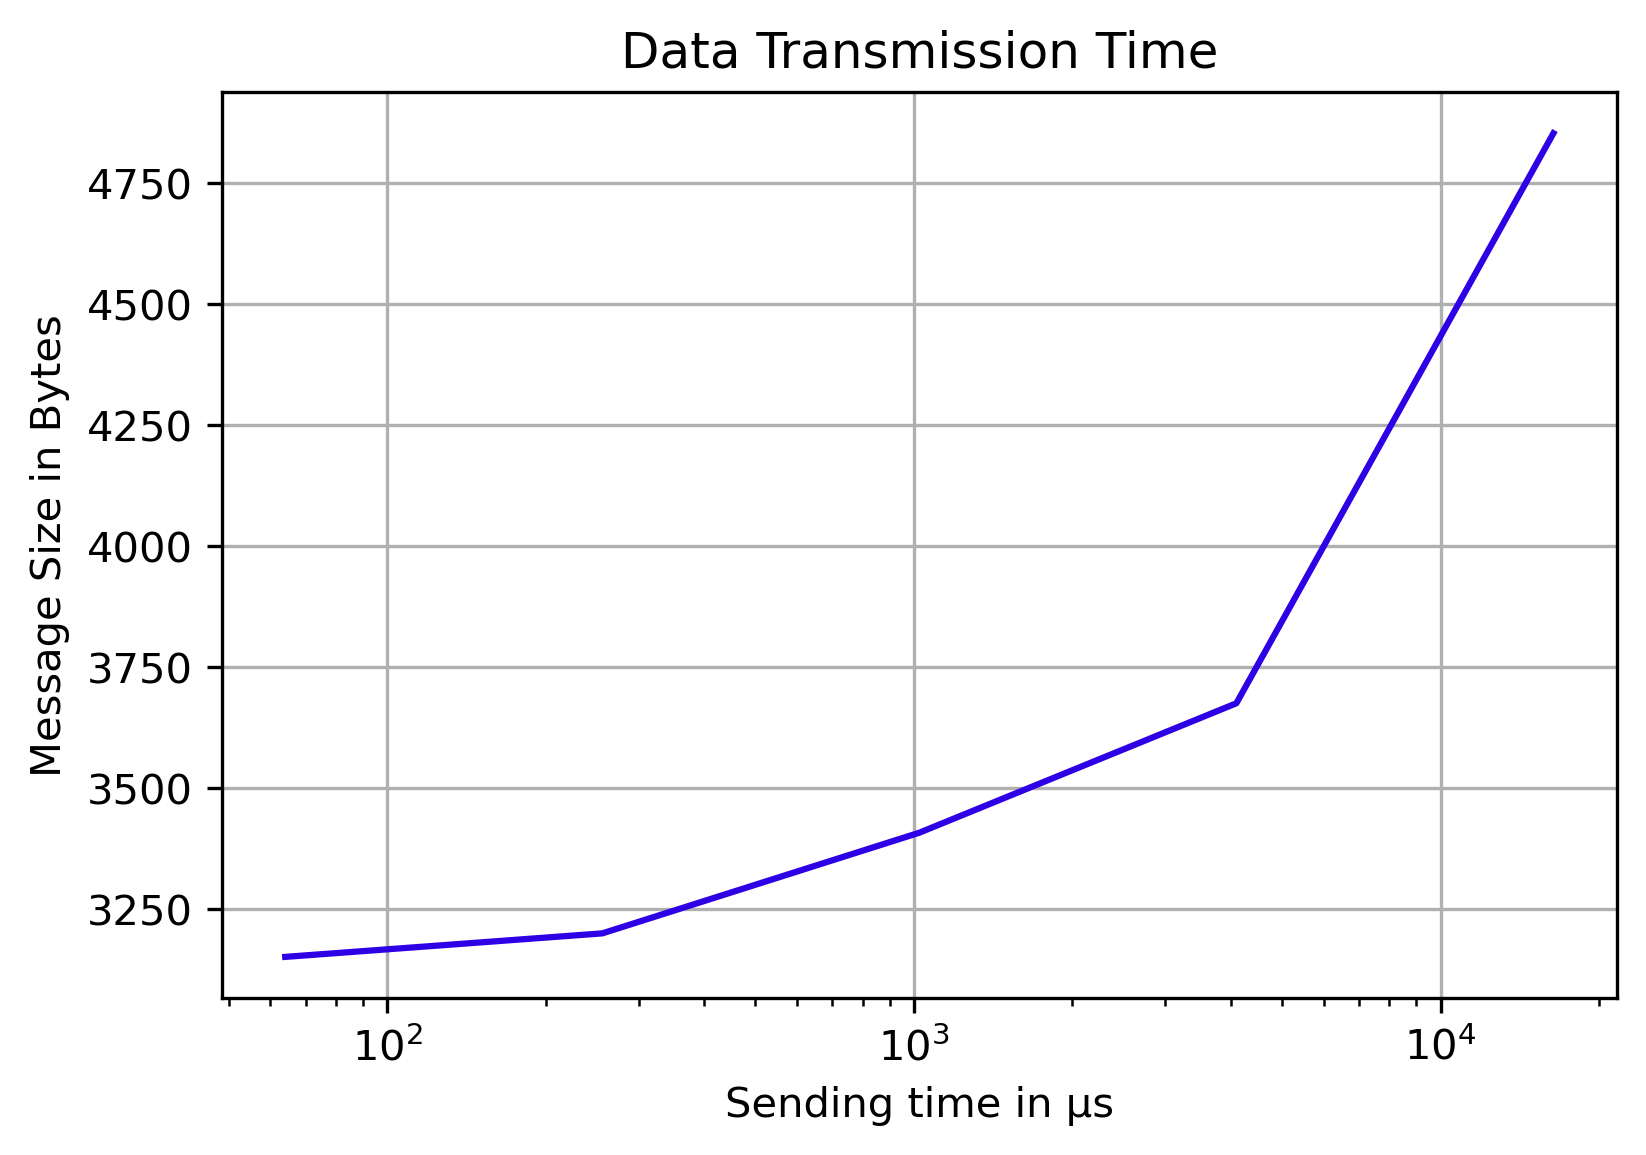
\includegraphics[width=0.75\linewidth]{images/plots/sendingTimes}
	\caption{Time that is required to transmit messages with different payload sizes via a \abr{DDS} topic. The times were determined by calculating the mean sending time out of 200 messages.}
	\label{fig:PlotSendingTimes}
\end{figure}


A end-to-end probing approach has been chosen over a \abr{IP} \abr{TTL} technique, which has been proposed by~\cite{SinhaMeasureNetworkLatency}, because the applied network has the same diameter for each node.
When a component publishes data to a \abr{DDS} topic, the middleware ensures that the data is transmitted to all registered subscribers.
In the system that is deployed for this thesis, data is transmitted via an \textit{Ethernet} connection.
The replicas are interconnected via a network switch that allows up to 2000 Mbit per seconds for each port.
In order to verify the applied topology the time that is required to send a message with a certain payload size between two replicas is measured.
For bypassing clock skews in the system, a request/response approach is used, where one replica publishes a message with a certain payload size and waits until a receiving replica confirms the message's receipt.
The receiving replica constantly checks for new messages and, as soon as it receives some, publishes a confirmation messages on another topic.
Any time that is required to send the confirmation message is negligible because it only consists of a 8-bit identification number, that assigns it to a payload carrying message.
The results, which are shown in~\cite{fig:PlotSendingTimes}, were determined by measuring the time that elapsed between sending a message and receiving the corresponding confirmation.
This process was repeated 200 times for each payload size and a mean was calculated.
What emerged is, that the transmission time is directly dependent on the published message's size.
\\

\begin{table}[h!]
	\begin{center}
		\caption{All topics that are utilized in the system have a certain data schema. From the resulting message size, the transmission time in the system can be calculated. The size and transmission time of the \texttt{AppendEntries} and \texttt{Input} depends on the length of the data sequence (\textbf{l}).}
		\label{tab:topicSendingTimes}
		\begin{tabularx}{\textwidth}{|X|X|X|}
			\hline
			\textbf{Topic} & \textbf{Message Size in Bytes} & \textbf{Expected Transmission Time in µs} \\
			\hline \hline
			AppendEntries & $12 + 4 * l$ & $0.402768 * l + 3219.11$ \\
			\hline
			AppendEntriesReply & 18 & 3219.7 \\
			\hline
			RequestVote & 8 & 3218.7 \\
			\hline
			RequestVoteReply & 13 & 3219.21 \\
			\hline
			Input & $4 + 4 * l$ & $0.402768 * l + 3218.3$ \\
			\hline
			ActivateSpare & 5 & 3218.40 \\
			\hline
			LinkedBalises & 6 & 3218.5 \\
			\hline
			TrainState & 41 & 3222 \\
			\hline
			MovementAuthority & 8 & 3218.7 \\
			\hline
		\end{tabularx}
	\end{center}
\end{table}

By the data size of the messages for the topics used in the system, the expected transmission times can be calculated.
These are listed in the~\autoref{tab:topicSendingTimes}.
The sizes are based on the \textit{Revolution Pi}'s system characteristics.
In ADLINK's \texttt{OpenSplice DDS}, the \textit{short} \abr{IDL} datatype resolves to a \textit{short int} C type, \textit{long} resolves to \textit{int} for the C programming language, \textit{unsigned long long} resolves to \textit{unsigned long long int}, and the \textit{boolean} datatype resolves to an \textit{unsigned char}.
A \textit{double} \abr{IDL} datatype resolves to an \textbf{double} C type.
The replica system's size characteristics for an \textit{short int} are two bytes, for an \textit{int} are four bytes, for an \textit{unsigned long long int} are eight bytes, for a \textit{double} are eight bytes, and for an \textit{unsigned char} is one byte.
The transmission time was calculated via the equation $transmissionTime(size) = 0.1100692 * size + 3217.9$ that has been derived by regression from~\autoref{fig:PlotSendingTimes}.
For the \texttt{AppendEntries} and \texttt{Input} topic, the actual data size and thereby the expected transmission time depend on the data sequence's length. 

\todo{Was bedeutet das für das konkrete System}

\paragraph{Idle Resource Utilization}
\begin{figure}[!hb]
	\centering
	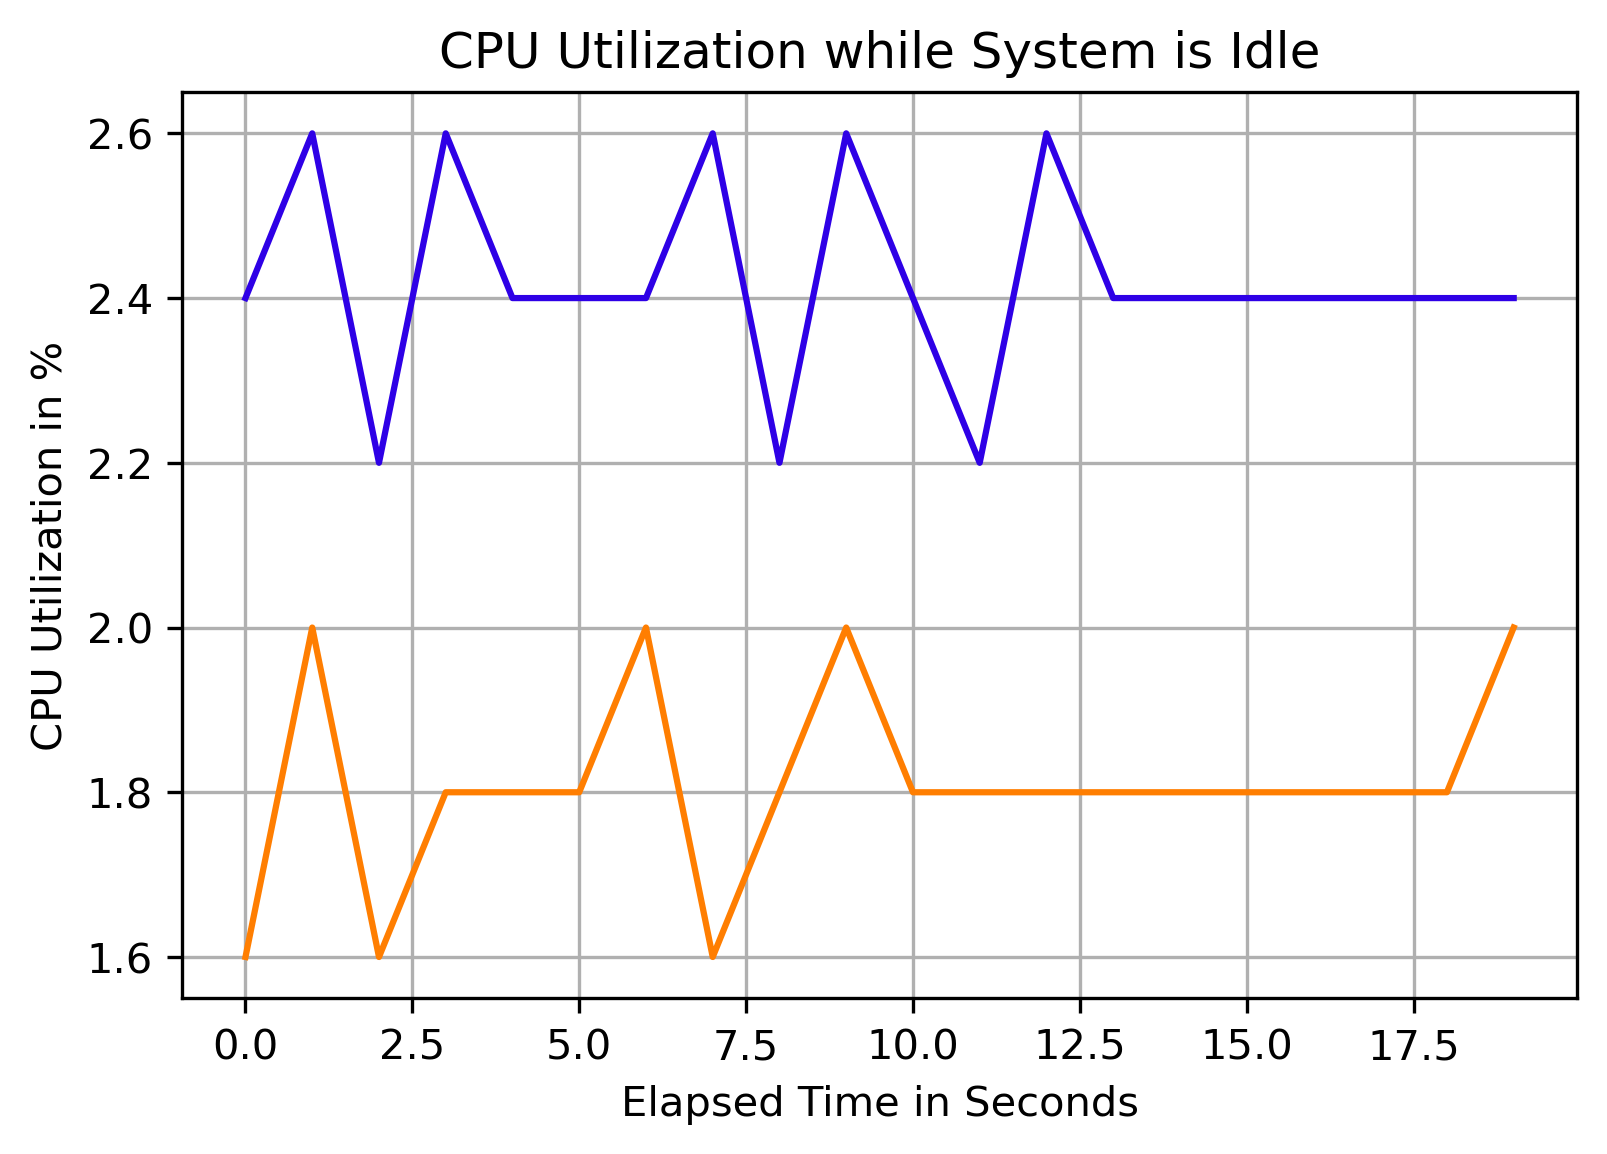
\includegraphics[width=0.75\linewidth]{images/plots/CPUUsageIdleTime}
	\caption{This plot shows the \glsentryfull{CPU} utilization in \% for both leader and follower in idle mode where only heartbeat messages are exchanged.}
	\label{fig:PlotCPUUsageIdleTime}
\end{figure}

In this paragraph, the utilized \abr{CPU} resources for leaders and followers are examined in both idle mode and when the system receives input messages.
Measurements were made with \textit{pidstat}, a tool that monitors individual tasks that are managed by the linux kernel.
\\

In idle mode, the train is not driving and only heartbeat messages are exchanged between the leader and its followers.
The \abr{CPU} usage for both a leader and a follower in idle mode are depicted in~\autoref{fig:PlotCPUUsageIdleTime}.
It can be seen that the utilization rate is consistently higher for the leader than for a follower.
On average, the follower utilized 1.81\% in 90 seconds, while the leader utilized 2.42\% of the applied \abr{CPU}.
In system mode, 0.21\% are used for the leader and 0.25\% for a follower on average.
For user mode, the leader utilizes on average 1.0\%, while a follower uses 0.66\%.
This can be explained by the fact that the leader has more responsibilities in idle mode.
It not only periodically sends heartbeat messages, but also observes whether the train has a valid \abr{MA} and can start driving.


\subsection{Scenario Simulation}
\todo{Redo all measurements in one scenario}
The simulated scenarios, that have been described in~\autoref{subsec:ScenarioSimulation}, are used for integration testing.
For this purpose, a functionality that writes the system's reactions to external factors into an evaluation file was patched into the on-board unit.
Said external factors include \abr{RBC} messages containing linking and \abr{MA} information, balise telegrams, as well as braking curve monitoring.
Every time the system reacts, the current position, the performed action, the encountered balise, and the reason for the action are listed.
A python script, that invokes the simulator and assesses the system's evaluation file, is used for automated integration testing.
\\

The following scenarios are supported and successfully processed by the replicated system:

\begin{table}[h!]
	\begin{center}
		\caption{A Python program is used for automatic integration testing. The scenarios that are traversed in the process differ in the relation of linked and unlinked balises and their expected outcome.}
		\label{tab:stateQOS}
		\begin{tabularx}{\textwidth}{|X|X|X|}
			\hline
			\textbf{Name} & \textbf{Number of balises/linked balises} & \textbf{Expected behaviour}\\
			\hline \hline
			Reach End of \abr{MA} & Three/Three & All balise telegrams are evaluated correctly and the train stops before the \abr{MA} ends. \\
			\hline
			Unlinked Balise & Three/Two & The train stops when the unlinked balise is encountered. \\
			\hline
			Balise not where expected & Three/Three & The actual position of one balise does not correspond with its linked position. The train stops when this balise is encountered. \\
			\hline
		\end{tabularx}
	\end{center}
\end{table}

Because the trips are simulated, a reproducible test environment is created.
The only non-deterministic factor is the synchronization of the individual components.
Further, the replica's hardware resources might not meet the scenarios and system's requirements. 
Therefore, the resource utilization, as well as message exchange and the \abr{DDS} feature's correct usage assessed.

\paragraph{Resource Utilization in Operation}

\begin{figure}[!hb]
	\centering
	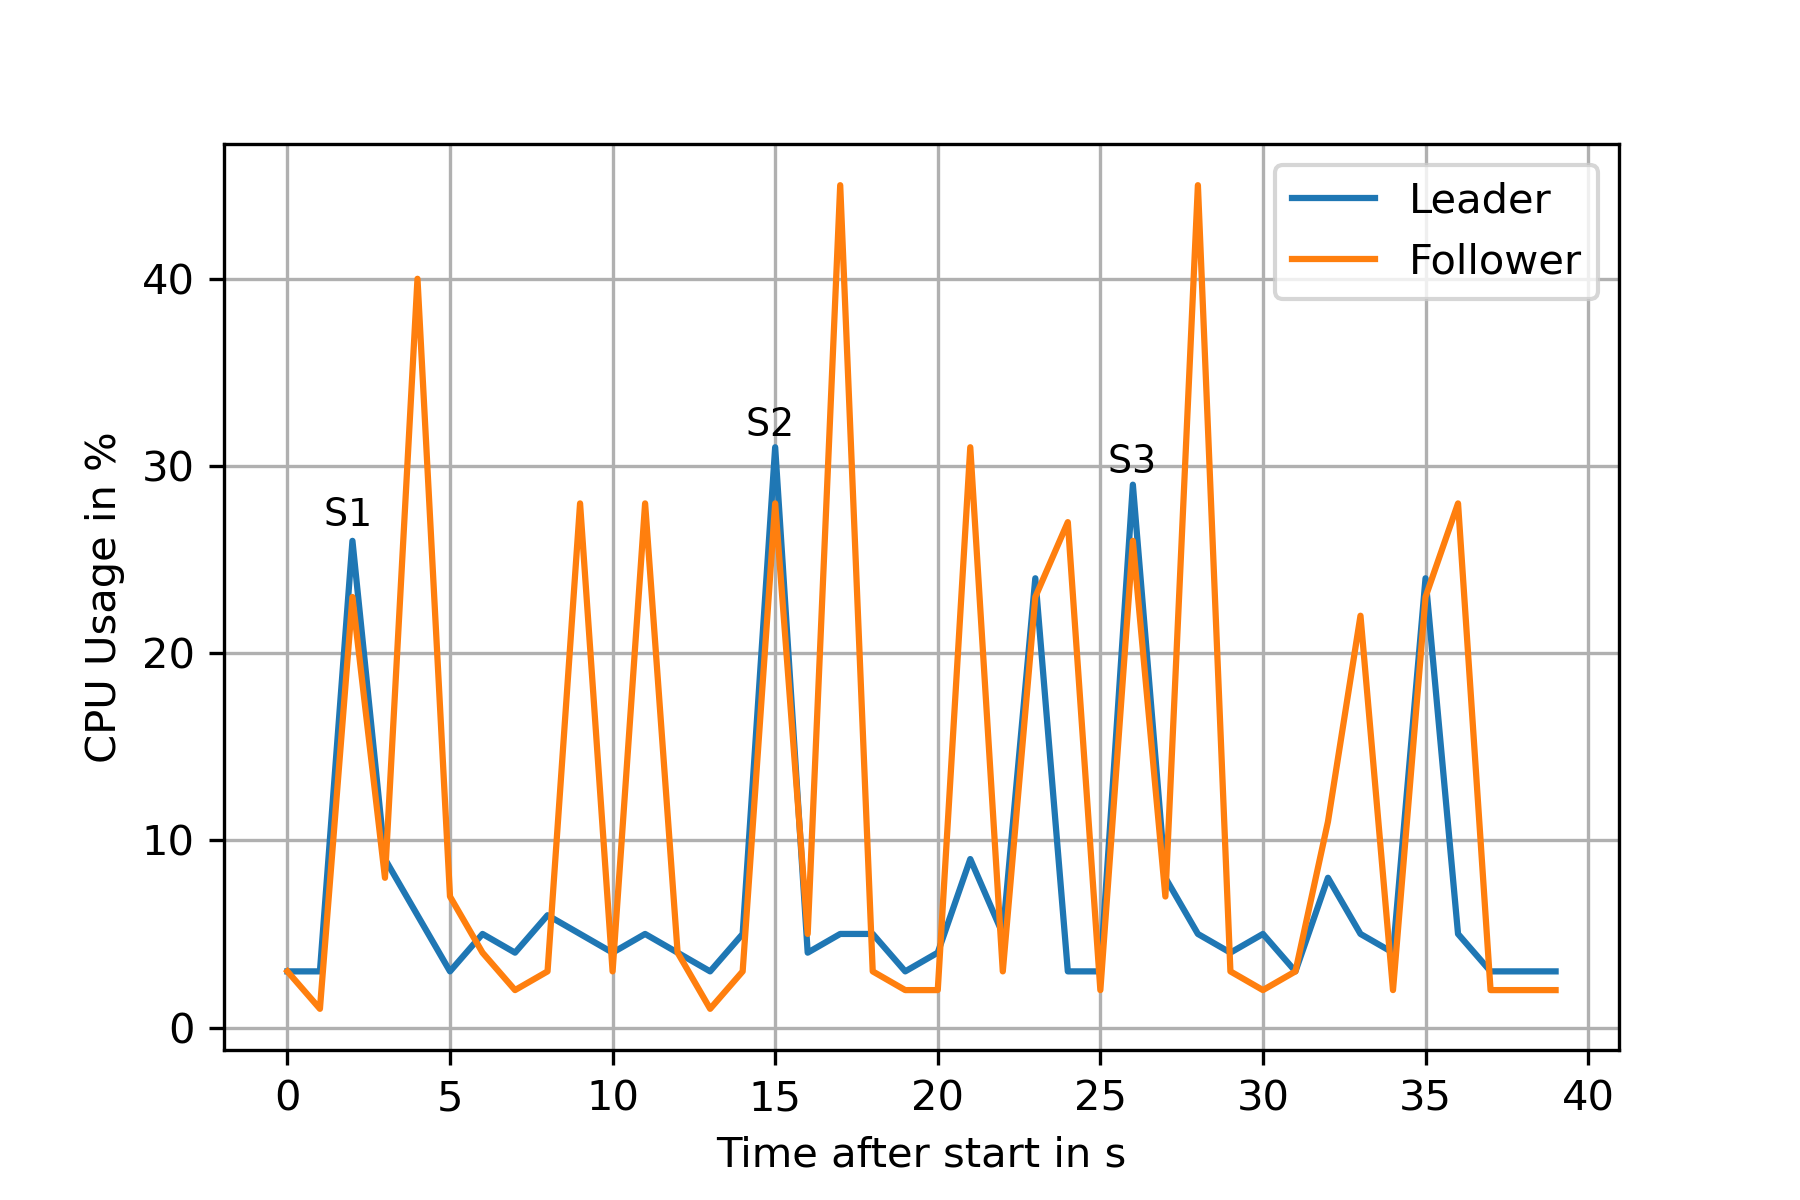
\includegraphics[width=0.75\linewidth]{images/plots/CPUUsage}
	\caption{This plot shows the \glsentryfull{CPU} utilization in \% for both leader and follower while the system receives and evaluates input messages.}
	\label{fig:PlotCPUUsage}
\end{figure}

The \abr{CPU} utilization when the system receives and evaluates input messages is depicted in~\autoref{fig:PlotCPUUsage}.
For this measurement, three scenarios, namely \texttt{Reach End of \abr{MA}}, \texttt{Unlinked Balise}, and \texttt{Balise not where expected} where run and \abr{CPU} utilization has been measured with \texttt{pidstat}.
On average, the leader utilizes 7.4\% of the applied \abr{CPU} resources, while a follower utilizes 12.675\% on average.
In system mode, 1.65\% are used for the leader and 1.05\% for a follower on average.
For user mode, the leader utilizes on average 5.73\%, while a follower uses 11.63\%.
\todo{Explain why follower might have higher CPU utilization}

The first scenario, \texttt{Reach End of \abr{MA}}, starts at 0 seconds.
The leader's first peak after two seconds (S1) is due to the balise and linking information of the first scenario being evaluated.
At the same time, the followers compare the train's braking curve with the new \abr{MA}, for which the \texttt{MovementAuthority} topic is accessed and the first peak on the follower side can be explained.
After four seconds, the follower has another peak in \abr{CPU} utilization.
At this point, the first balise is encountered and the train's position is compared to the linked balises.
Therefore, the train's state and the linked balises are retrieved for the first time from the topic, which together with the decision making leads to a high computational overhead.
The third and fourth peak (after nine and eleven seconds) are again due to an evaluated balise telegram.
However, only the updated train state is retrieved.

The seconds scenario \texttt{Unlinked Balise} (\textbf{S2}) starts after 15 seconds.
The peaks, again, can be explained by data publication and retrieval.
At 23 seconds after the measurements started, an unlinked balise is encountered and the train needs to stop.
This leads to an increase in \abr{CPU} utilization for both the leader and the followers.

The third scenario \texttt{Balise not where expected} (\textbf{S3}) starts at 26 seconds.
At 35 seconds after the measurements were started, an unexpected balise has been encountered, which can be seen in the graph as well.

\subsubsection{Message Exchanges}
\todo{Mention that no spare activation happens in the measurements}
As the scenarios are run, messages are exchanged between the replicas via the different \abr{DDS} topics.
For the message exchange evaluation, the leader has been manually stopped after the second scenario and before the third scenario is run.
The third scenario has been run with only a leader and one follower.
In the following, the number of messages that occur during the simulation of the three successive scenarios, that were described above, is analyzed.
At first, the sent messages are examined.
Therefore, the total number of sent messages, as well as the number of messages for the consensus topics and the state topics are analyzed.
Afterwards, the same is done for the received messages.
Besides the topics named above, the \texttt{Input} topic will be taken into account for the received messages.

For each measurement, the heartbeat timer has been set to 100000µs so that ten messages per second can be attributed to heartbeat messages.

\paragraph{Total Messages Sent}

\begin{figure}[!hb]
	\centering
	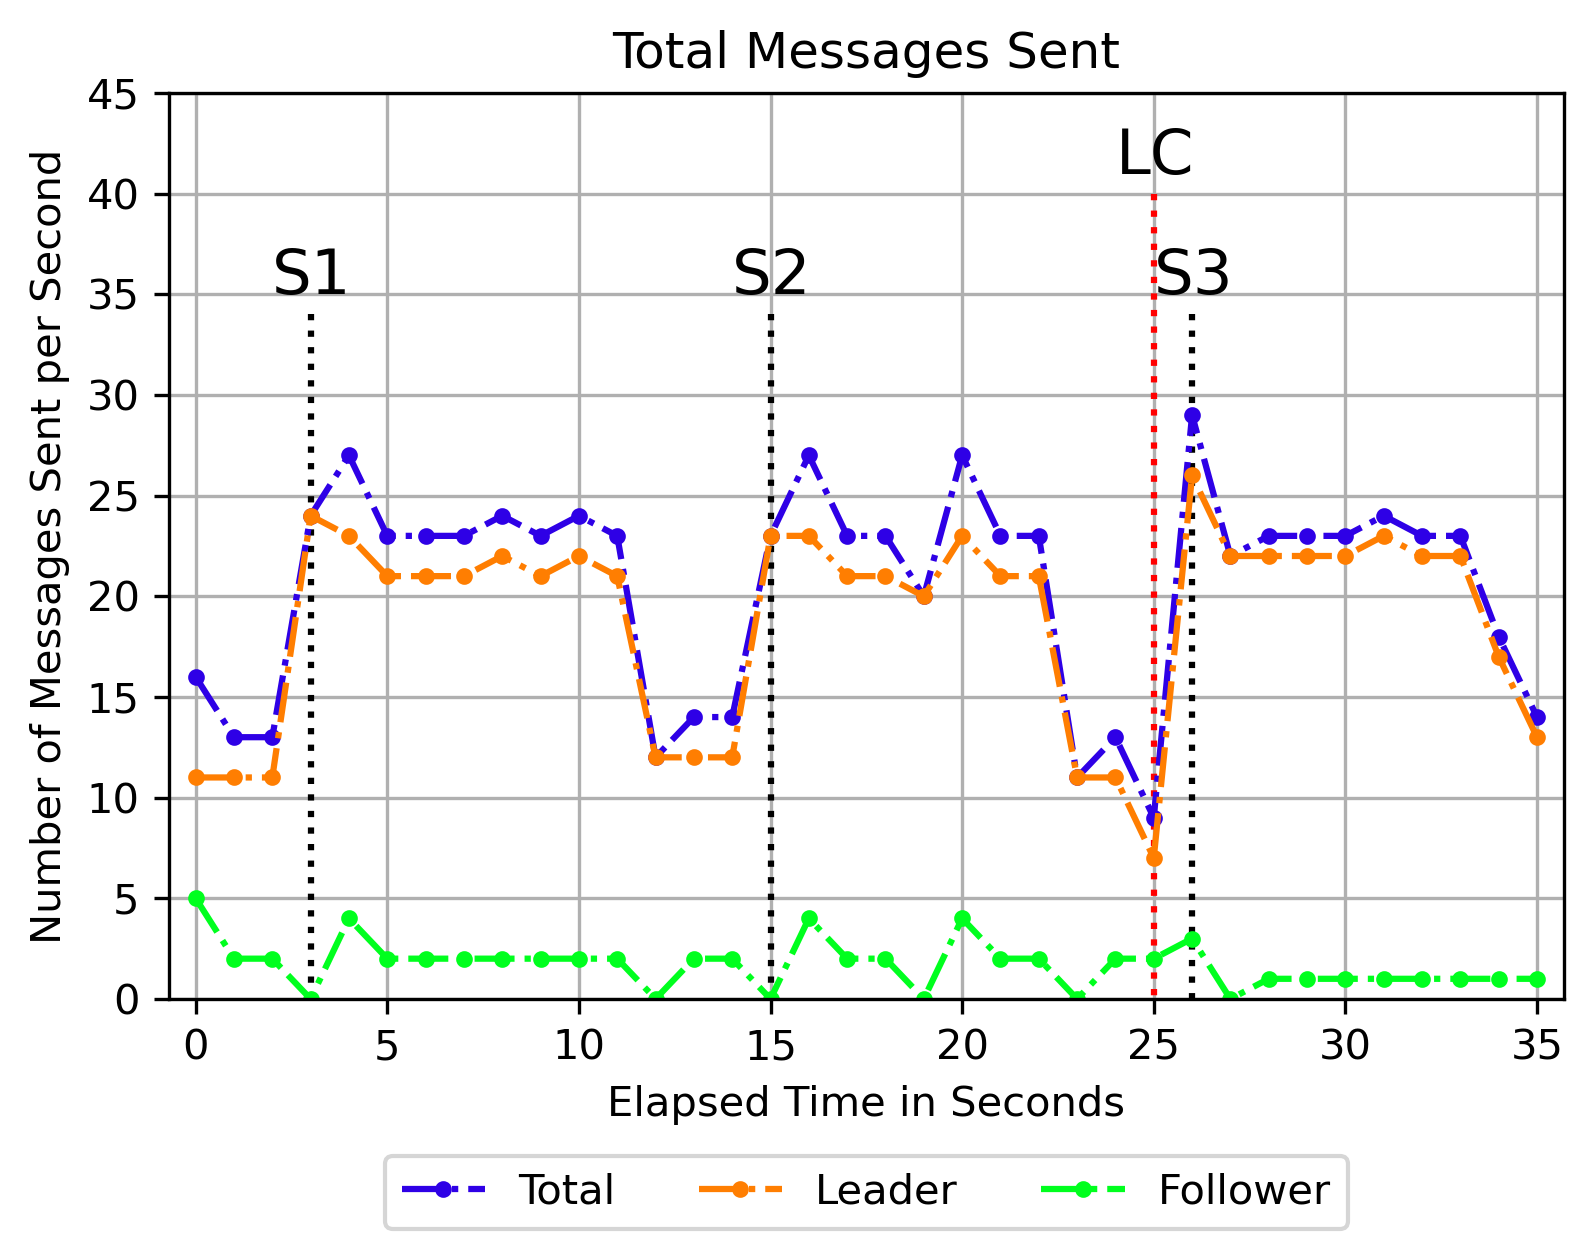
\includegraphics[width=0.75\linewidth]{images/plots/TotalMessagesSent}
	\caption{Overview about sent messages in the system. A distinction is made between the messages that are send by the system's leader and the followers . In addition, the overall number of sent messages is shown.}
	\label{fig:PlotTotalMessagesSent}
\end{figure}

The total number of messages that were sent by replicas in the system per seconds are shown in~\autoref{fig:PlotTotalMessagesSent}.
Beginning and end of each of the three scenarios can be seen in the plot because the total number of sent messages increases to 20-25 messages per second while driving and reduces to twelve messages per second when the train stands still.
A majority of messages is sent by the system's leader of which ten alone are due to heartbeat messages.
The rest accrue from cluster-wide monitoring of the braking curve.
While the train is driving, it is the leader's responsibility to update the system's global state which explains the big increase in sent messages during journey.

\paragraph{Consensus Messages Sent}

\begin{figure}[!hb]
	\centering
	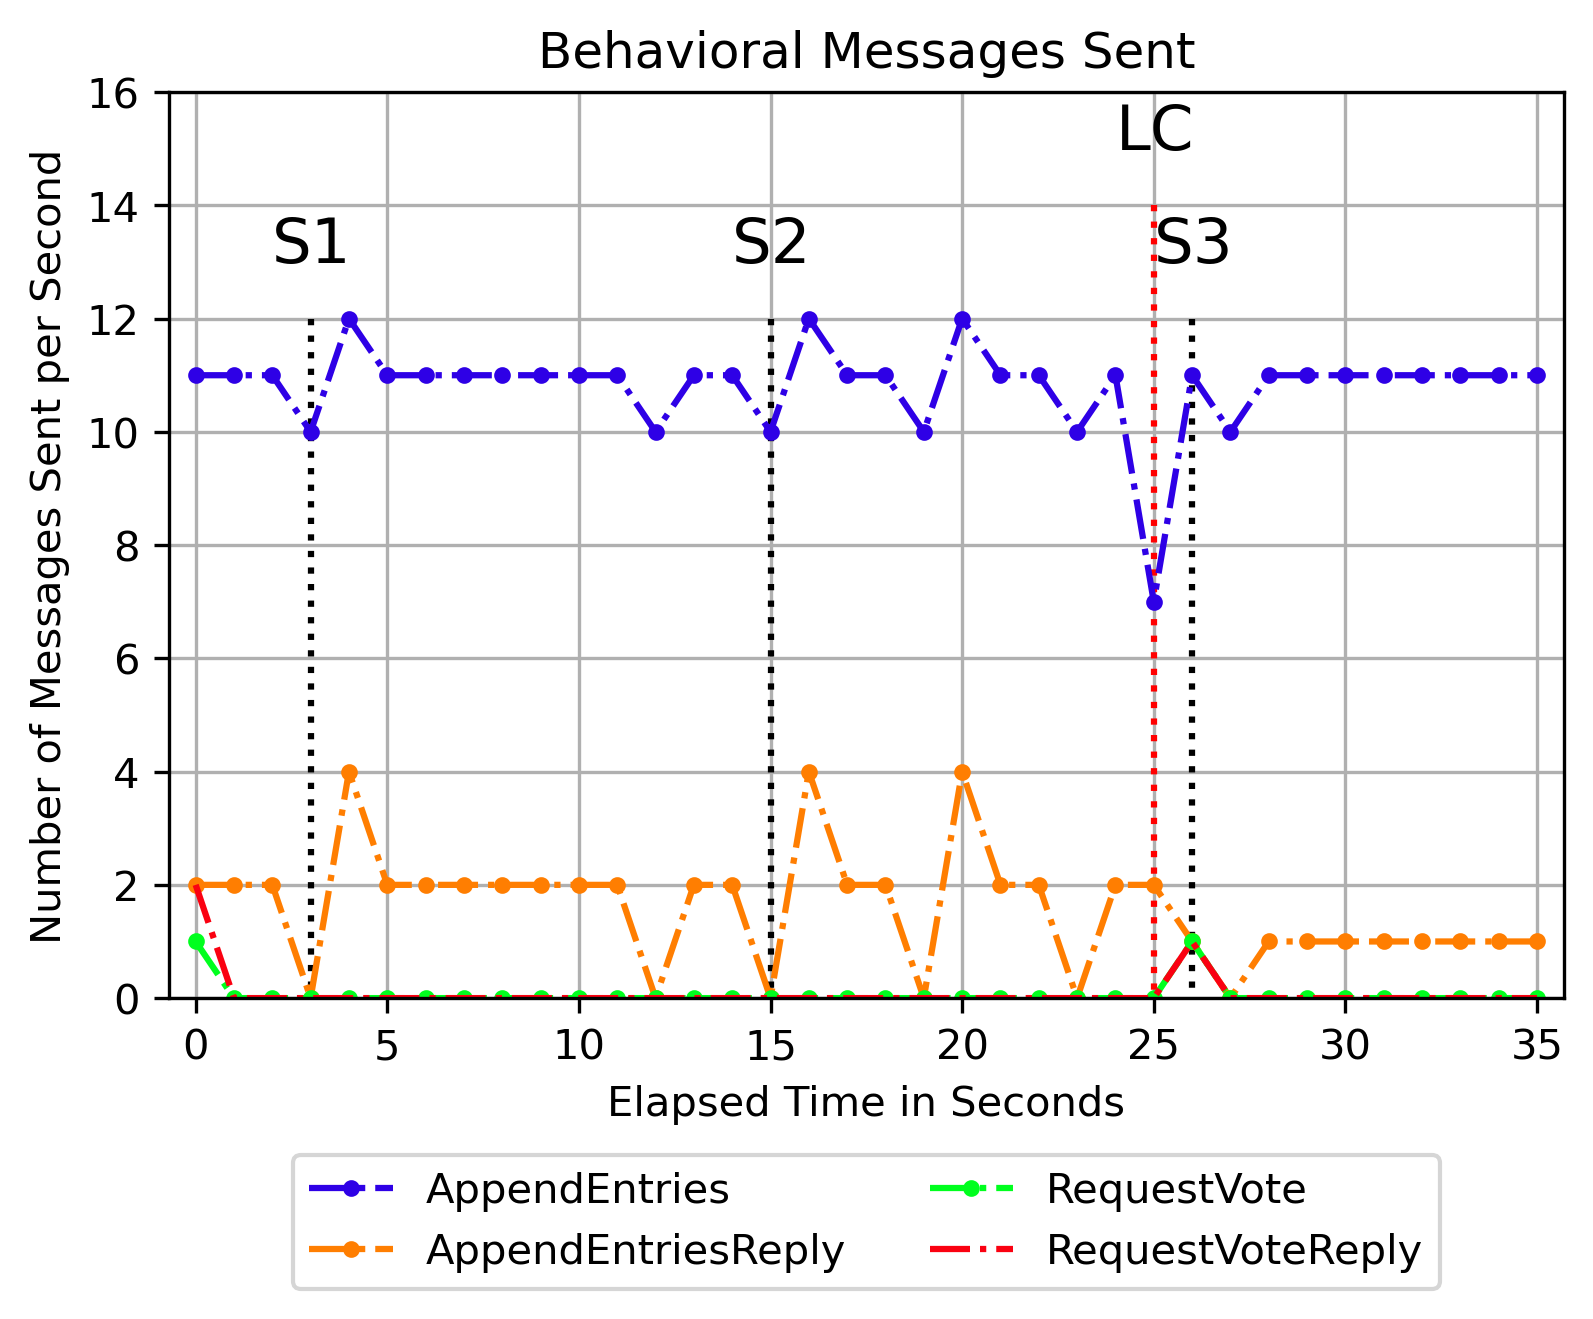
\includegraphics[width=0.75\linewidth]{images/plots/ConsensusMessagesSent}
	\caption{The sent messages for all topics used for the consensus algorithm. \texttt{AppendEntries} is used for heartbeat messages and for log replication. \texttt{AppendEntriesReply} functions as a way to transmit decisions from followers to the leader. Via \texttt{RequestVote} and \texttt{RequestVoteReply}, the leader voting happens. After 25 seconds, the previous leader crashes, which results in a drop of heartbeat messages in the \texttt{AppendEntries} topic. After a new leader is elected, the amount of heartbeat messages goes back to the previous one.}
	\label{fig:PlotConsensusMessagesSent}
\end{figure}

Consensus topics include \texttt{AppendEntries}, \texttt{AppendEntriesReply}, \texttt{RequestVote}, and \texttt{RequestVoteReply}.
The number of messages published to the consensus topics are depicted in~\autoref{fig:PlotConsensusMessagesSent}.
The majority of messages gets published to the \texttt{AppendEntries} topic, because the leader periodically published ten heartbeat messages per second.
It can be seen that a leader election takes place at the beginning, because a vote request and two vote replies are sent.
Another leader election happens after the second scenario has finished after 25 seconds.
The fact that the previous leader crashed is reflected in the collapse of heartbeat messages on the \texttt{AppendEntries} topic.
Again, a vote request is published to the corresponding topic by the first replica that notices the absent leader.
This time, only one vote reply is published because only one other replica remains in the system.
The new leader establishes itself afterwards because the amount of heartbeat messages goes back to the number it was before the previous leader crashed.


\paragraph{State Messages Sent}

\begin{figure}[!hb]
	\centering
	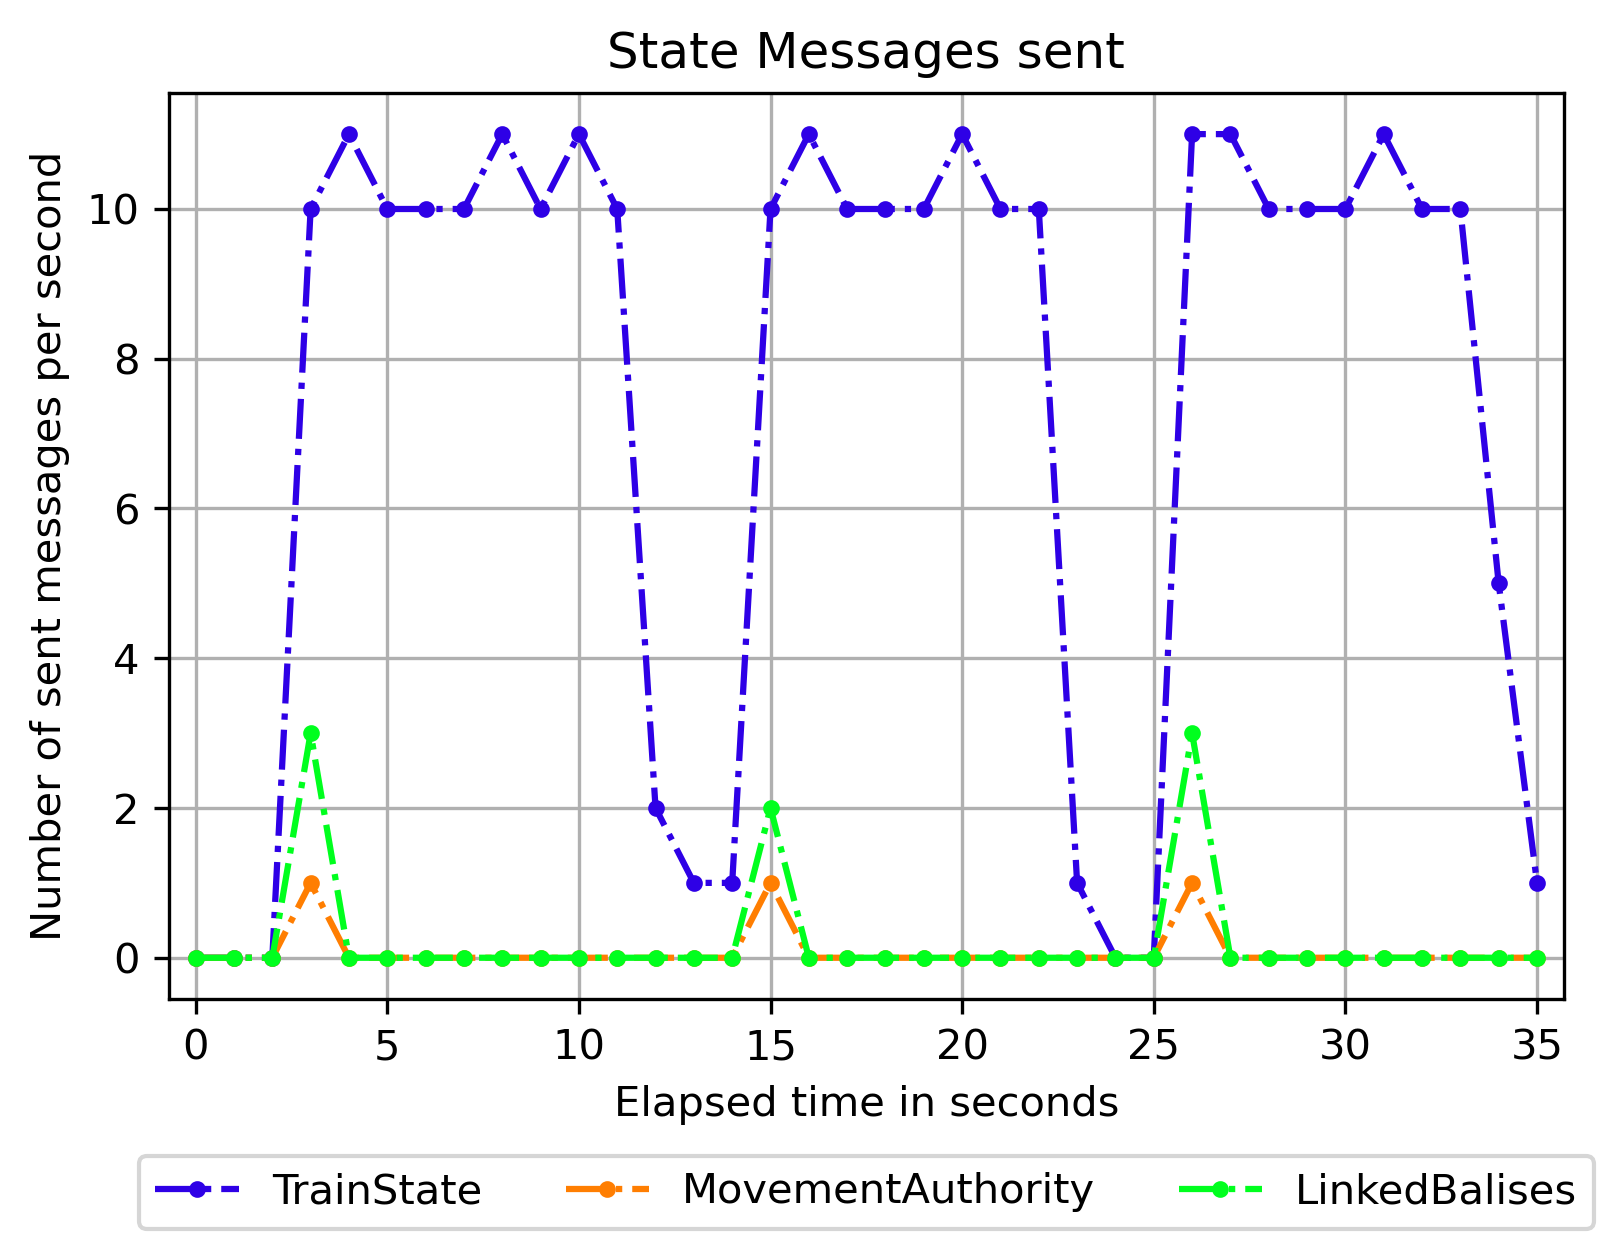
\includegraphics[width=0.75\linewidth]{images/plots/StateMessagesSent}
	\caption{The sent messages for the topics that store the system's global state. It can be seen that, at the beginning of each scenario, a new \glsentryfull{MA} and linked balises are stored. The train's position is simulated and updated every 100ms in the \texttt{TrainState} topic.}
	\label{fig:PlotStateMessagesSent}
\end{figure}

State topics include \texttt{TrainState}, \texttt{MovementAuthority}, and \texttt{LinkedBalises}.
The amount of messages published to these topics can be seen in~\autoref{fig:PlotStateMessagesSent}.
These messages are all sent by the leader, because it is the only replica that is allowed to publish to these topics.
It is noticeable that most state messages are published on the \texttt{TrainState} topic.
This is because the position is simulated every 100000µs and written to \texttt{TrainState}.
The small peaks for the \texttt{TrainState} topic indicate that the train's position is reset when the train encounters a linked balise.
Messages to \texttt{MovementAuthority} and \texttt{LinkedBalises} are only published at the beginning of each scenario, because at this time the \abr{MA} and linked balises are communicated to the system.
It can futher easily be seen that three balises are linked in the first and the third scenario but only two linked balises are added for the second.

\paragraph{Total Messages Received}

\begin{figure}[!hb]
	\centering
	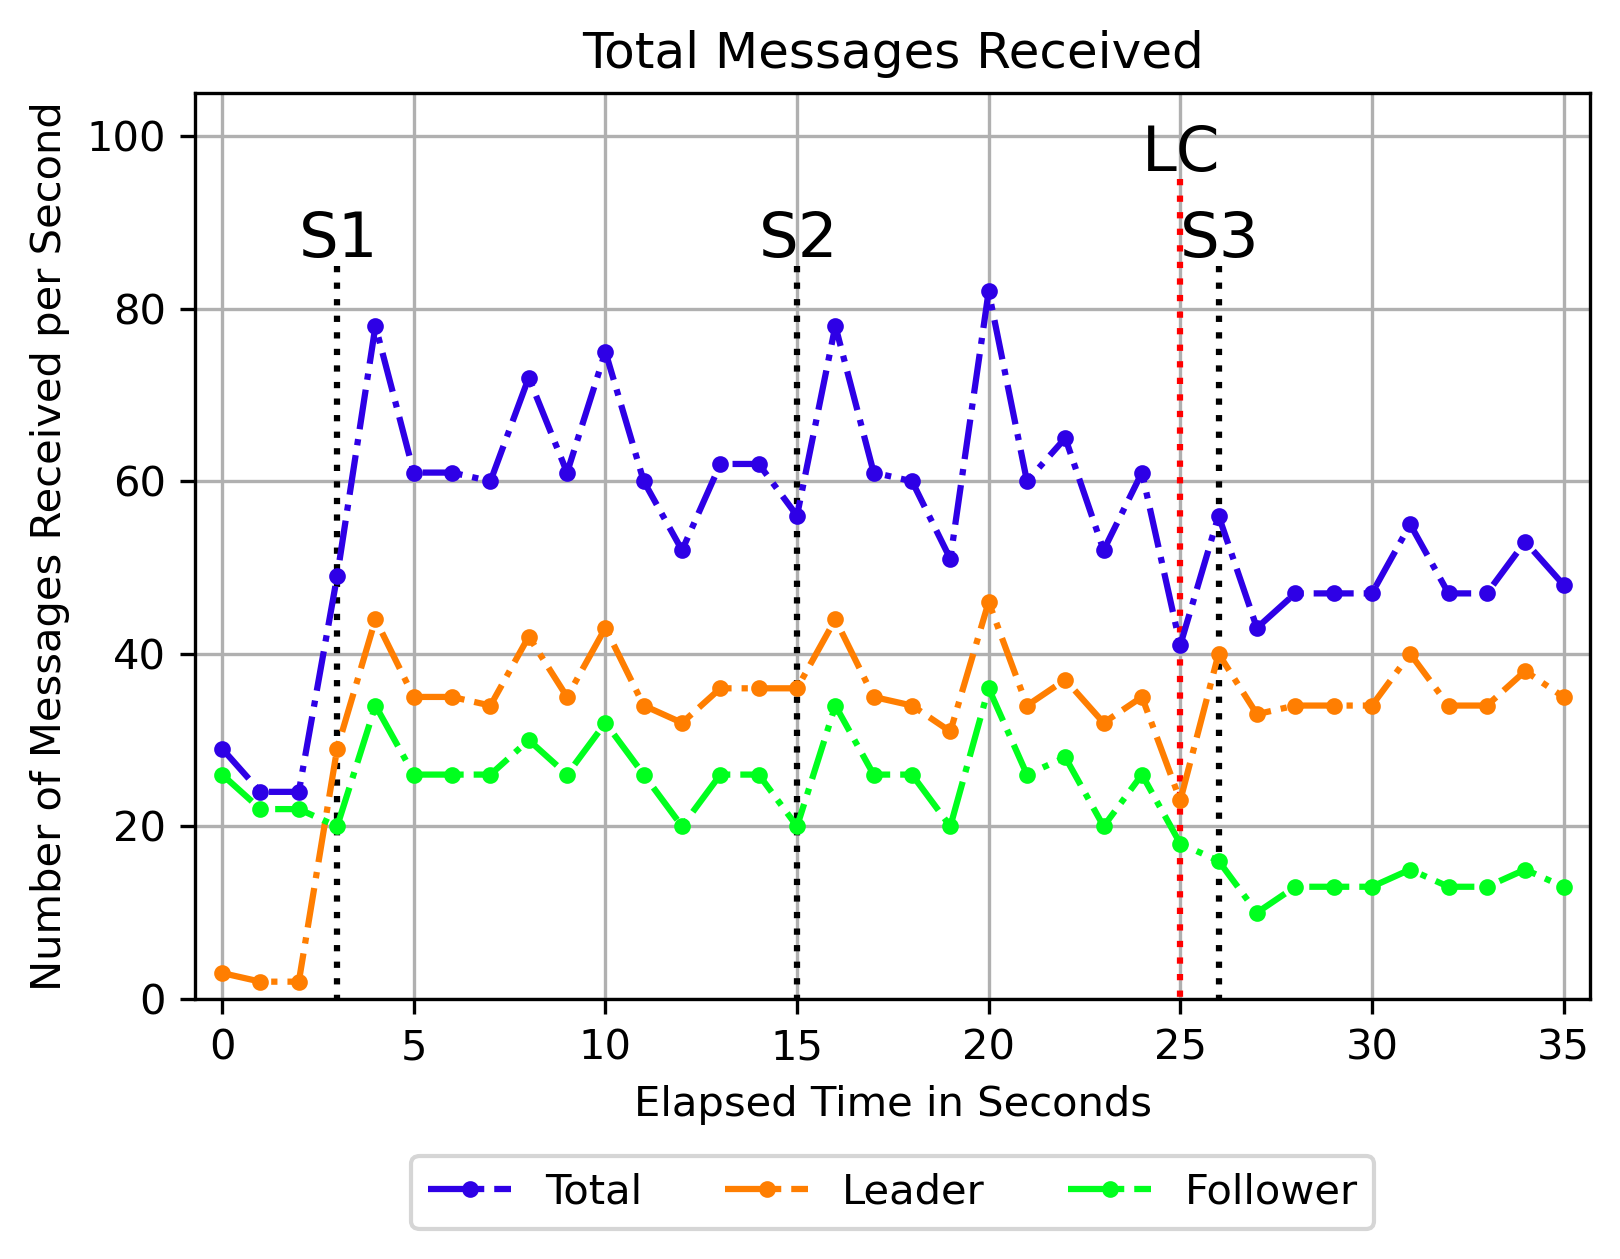
\includegraphics[width=0.75\linewidth]{images/plots/TotalMessagesReceive}
	\caption{Overview about all messages that are received from replicas within the system.}
	\label{fig:PlotTotalMessagesReceive}
\end{figure}

The total number of messages received through \abr{DDS} topics can be seen in~\autoref{fig:PlotTotalMessagesReceive}.
What is interesting is, that the leader receives and reads more messages than the two followers combined.
This is mostly because the leader is responsible for reading the input topic and because it receives and reads messages from both followers.
Another interesting circumstance can be seen after 25 seconds - which is when the previous leader crashes - since the amount of messages that the followers received is halved.
This is because only one, instead of two, followers remain in the system.

\paragraph{Input Messages Received}

\begin{figure}[!hb]
	\centering
	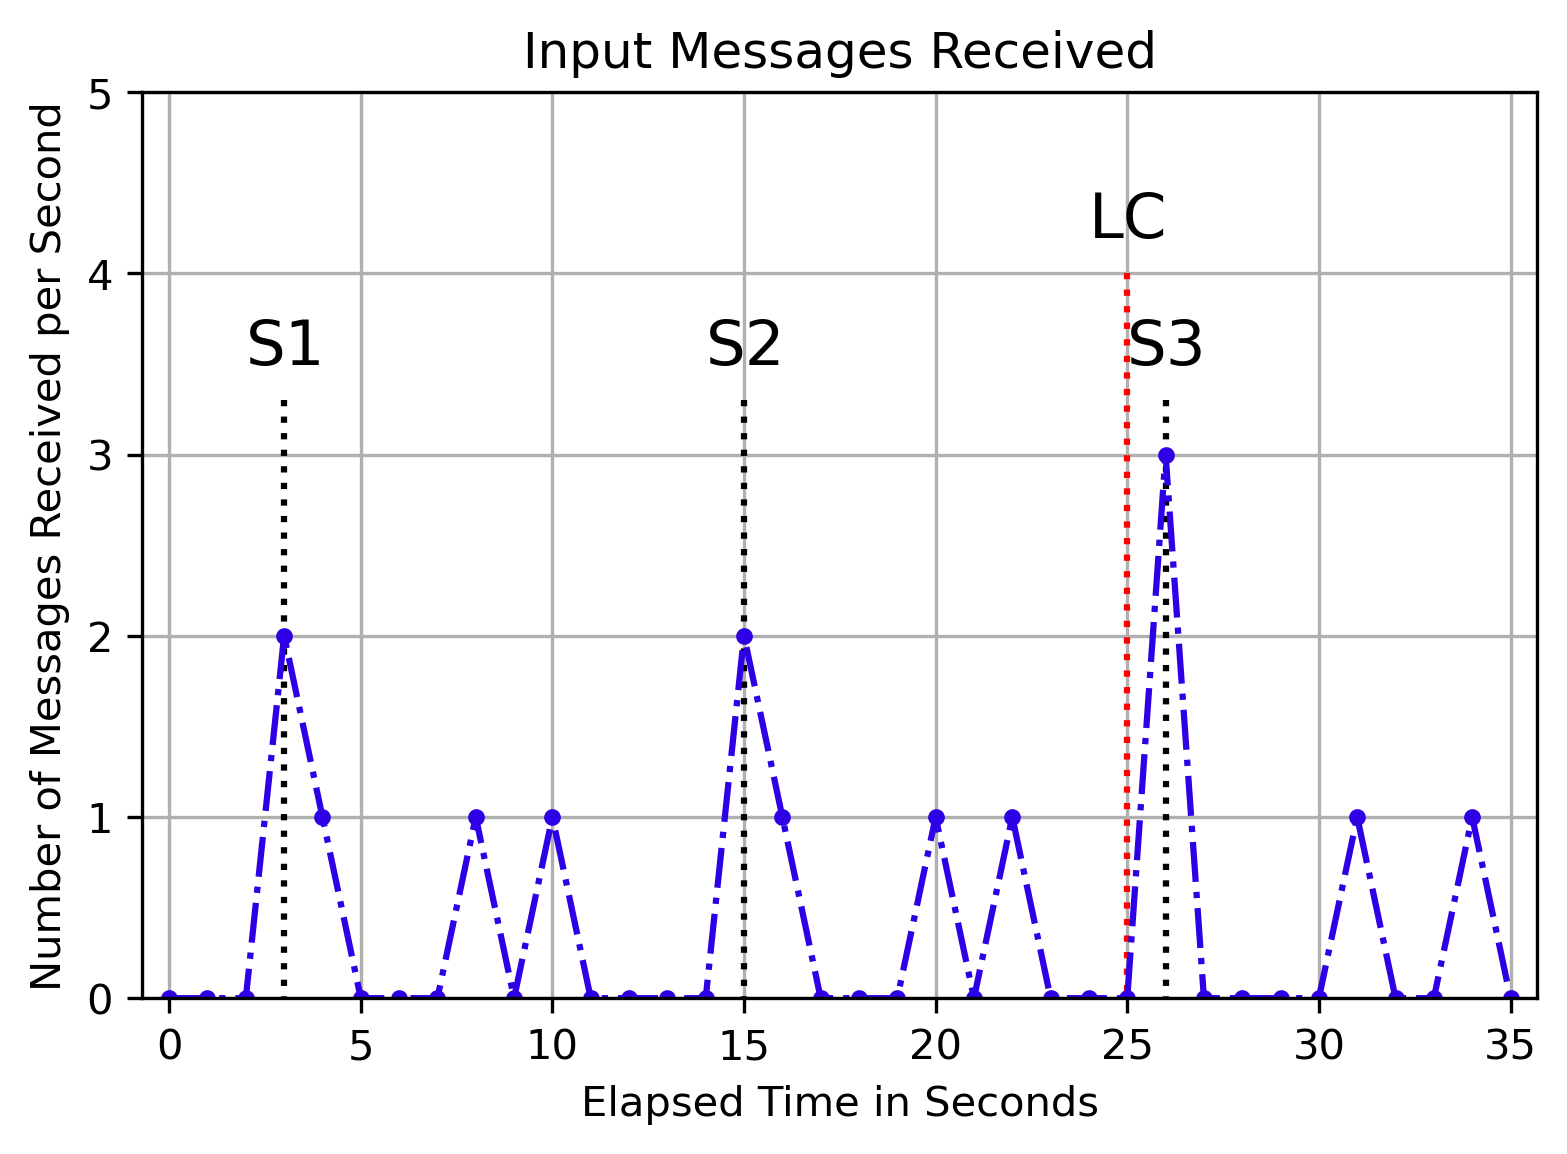
\includegraphics[width=0.75\linewidth]{images/plots/InputMessagesReceive}
	\caption{The number of input messages received by the system per second. Based on the distribution the scenarios procedure can be seen. At the beginning, two input messages contain the \glsentryfull{MA} and linked balises. One second later, the first balise telegram is received. The last two balise telegrams follow each other at an interval of two seconds. The distance between the last two balises is greater for the last scenario. This is because the last scenario, it is simulated that the balise is not at the position that was specified in the linking phase.}
	\label{fig:PlotInputMessagesReceive}
\end{figure}

The individual scenarios' structures can be traced by the input messages that the sytem receives.
This is depicted in~\autoref{fig:PlotInputMessagesReceive}.
At the beginning of each scenario, one message with the \abr{MA} and one with the linked balises are sent.
Because the train's speed is simulated to be constant, the intervals between the incoming balises telegrams are the equal for the first and the second scenario.
In the third scenario it is simulated that the last balise is at a different position than specified in the linking phase.
Therefore, the distance between the last two balises is greater in the third scenario.
It can also be seen that although after 25 seconds the old leader crashes, the system does not miss any input message.
However, unlike the first two scenarios, the input messages are buffered and therefore processed all at once, which is why the peak is higher.

\paragraph{Consensus Messages Received}

\begin{figure}[!hb]
	\centering
	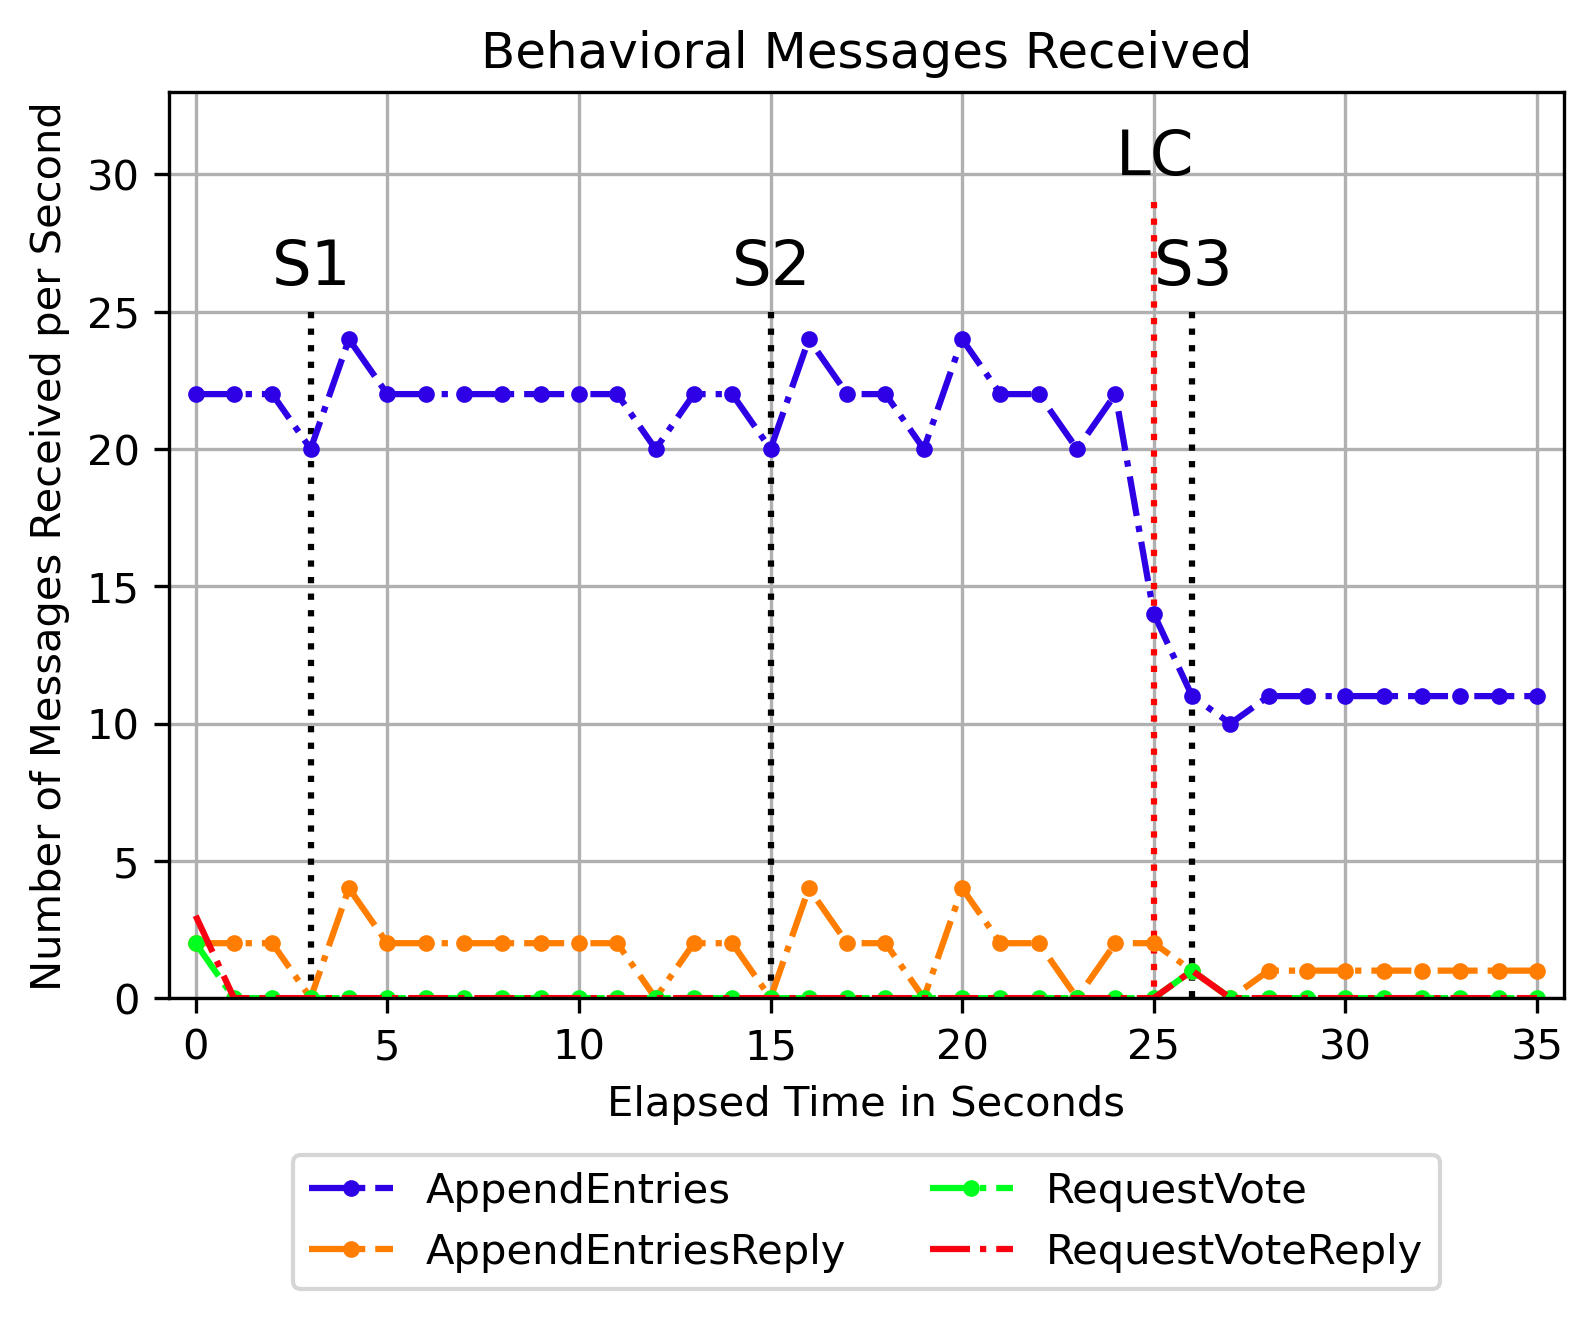
\includegraphics[width=0.75\linewidth]{images/plots/ConsensusMessagesReceive}
	\caption{All messages that are received by a component on the topics used for finding a consensus. After 25 seconds, a new leader is elected and only one follower remains in the system. Therefore, messages are read from \texttt{RequestVote} and \texttt{RequestVoteReply}. Further, since the number of followers got reduced by half, also the number of received heartbeat messages got reduced.}
	\label{fig:PlotConsensusMessagesReceive}
\end{figure}

The number of received messages on the consensus topics is shown in~\autoref{fig:PlotConsensusMessagesReceive}.
It is noticeable that after 25 seconds the number of AppendEntries messages received drops.
Further, a message is received on the \texttt{RequestVote} and on the \texttt{RequestVoteReply} topic, respectively.
From this it can be seen that a leader election occurred.
Because there is only one follower left in the system, the number of received heartbeat messages is halved.


\iffalse
\paragraph{State Messages Received}

\begin{figure}[!hb]
	\centering
	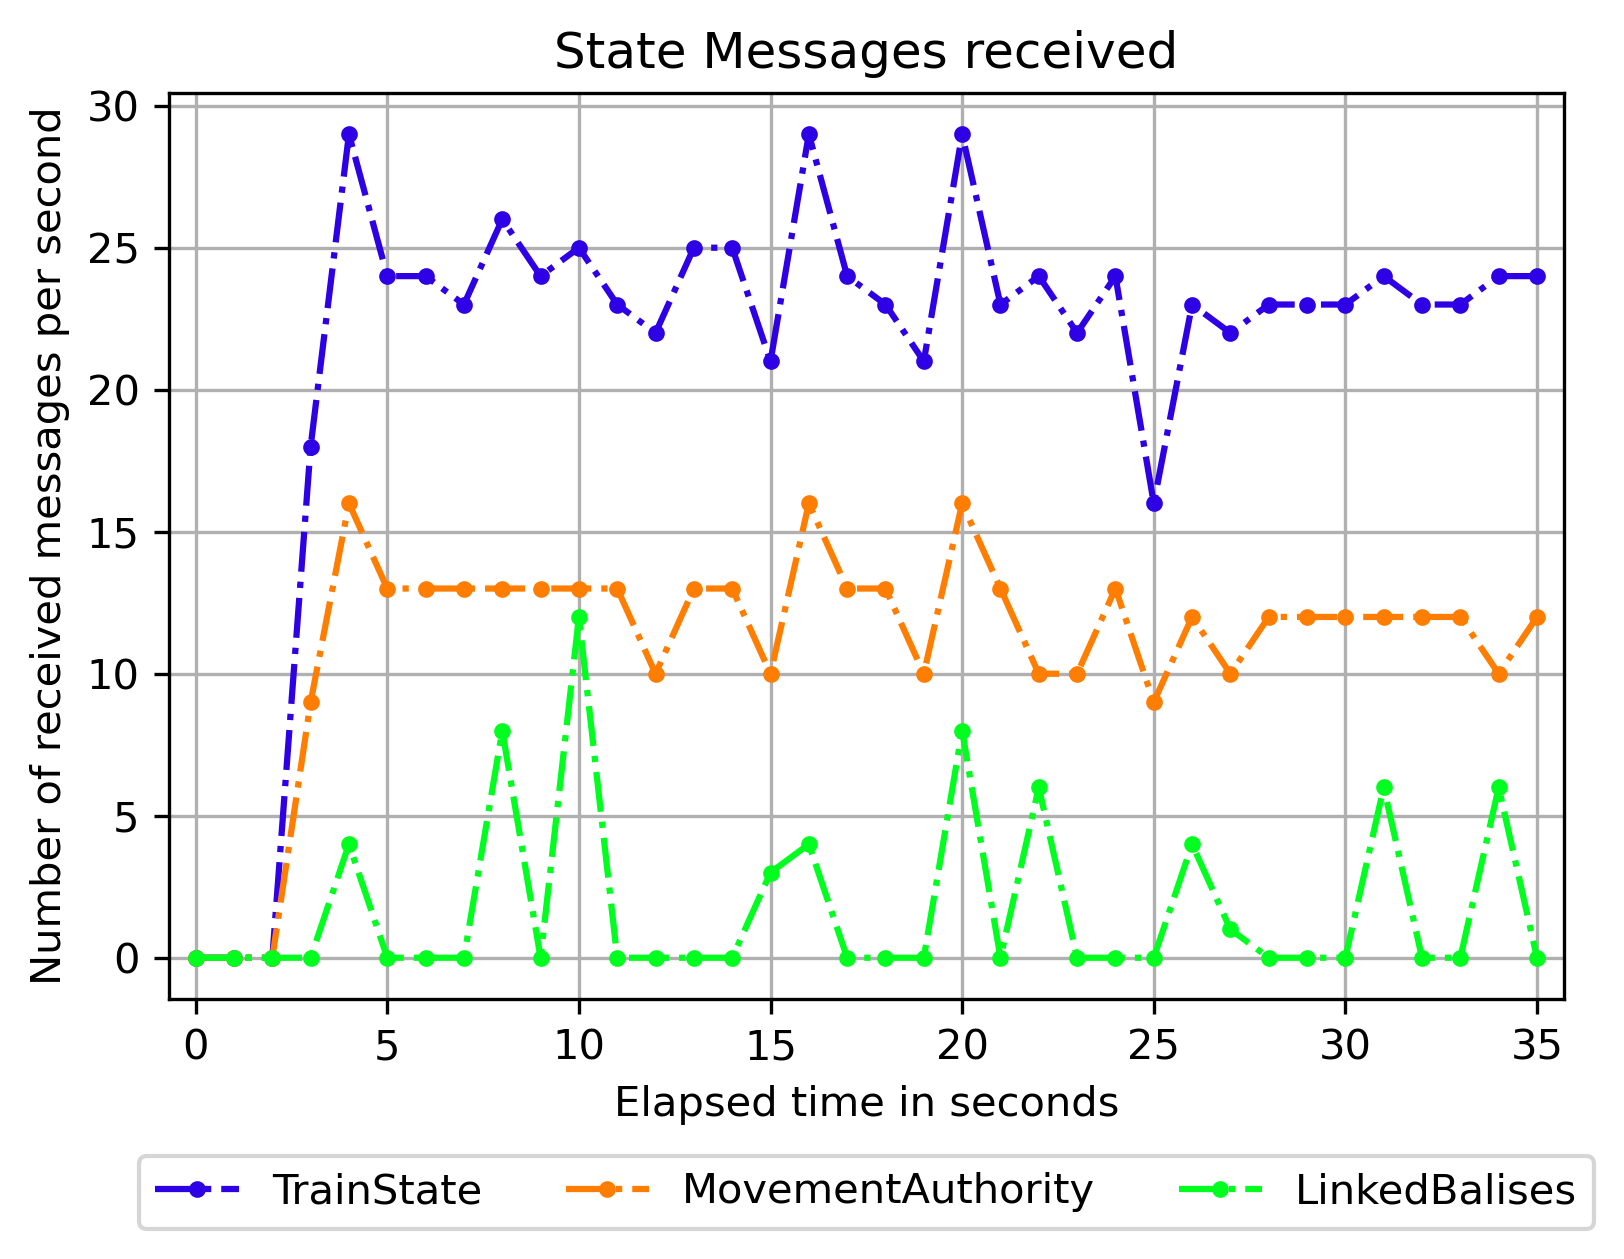
\includegraphics[width=0.75\linewidth]{images/plots/StateMessagesReceive}
	\caption{}
	\label{fig:PlotStateMessagesReceive}
\end{figure}

\todo{Do measurement with killing leader, but this time activate spare and show a topic selection that hot standby works}

Do experiement and structure in way such as SakicTimeInConsensus

Leader stable for 45 minutes with 500000x07x2

For the tranmit time, I measured 20 messages each time and took the average (calculate standard deviation)
\fi

    
	% Bibliographie
	\ifisbook\cleardoubleemptypage\fi
	\phantomsection\addcontentsline{toc}{chapter}{\refname}
	\printbibliography[category=cited]

	% ggf. Anhang
	% \appendix\chapter{\appendixname}

\section*{Eins (ohne extra Eintrag im Inhaltsverzeichnis)}
Lorem ipsum dolor sit amet, consetetur sadipscing elitr, sed diam nonumy eirmod tempor invidunt ut labore et dolore magna aliquyam erat, sed diam voluptua. At vero eos et accusam et justo duo dolores et ea rebum.

\section*{Zwei (ohne extra Eintrag im Inhaltsverzeichnis)}
Stet clita kasd gubergren, no sea takimata sanctus est Lorem ipsum dolor sit amet. Lorem ipsum dolor sit amet, consetetur sadipscing elitr, sed diam nonumy eirmod tempor invidunt ut labore et dolore magna aliquyam erat, sed diam voluptua.

\section*{Drei (ohne extra Eintrag im Inhaltsverzeichnis)}
At vero eos et accusam et justo duo dolores et ea rebum. Stet clita kasd gubergren, no sea takimata sanctus est Lorem ipsum dolor sit amet.

\section*{Vier (ohne extra Eintrag im Inhaltsverzeichnis)}
Stet clita kasd gubergren, no sea takimata sanctus est Lorem ipsum dolor sit amet. % example

	% ggf. bei englischen Arbeiten den deutschen Abstract nach hinten verschieben
	% \ifisbook\pagestyle{plain}\cleardoubleemptypage\include{content/abstract_deu}\fi

	% Eigenständigkeitserklärung
	% \ifisbook\pagestyle{plain}\cleardoubleemptypage% => Laut Aussage des Studienreferats braucht es - auch wenn die Arbeit in englischer Sprache verfasst ist - KEINE separate Version der Eigenständigkeitserklärung auf Englisch. Sowohl für Arbeiten in deutscher Sprache als auch für Arbeiten in englischer Sprache genügt EINE EINZIGE Eigenständigkeitserklärung auf DEUTSCH.
\begin{otherlanguage}{ngerman}

\begin{center}\textsf{\textbf{Eidesstattliche Erklärung}}\end{center}
Hiermit versichere ich, dass meine Masterarbeit \enquote{\hpititle} (\enquote{\hpititleother}) selbständig verfasst wurde und dass keine anderen Quellen und Hilfsmittel als die angegebenen benutzt wurden. Diese Aussage trifft auch für alle Implementierungen und Dokumentationen im Rahmen dieses Projektes zu.\\

\noindent
Potsdam, den \hpidate,
\vspace{2cm}

\begin{center}
\begin{tabular}{C{6cm}}
\hline
{\small({\hpiauthor})}
\end{tabular}
\end{center}

\end{otherlanguage}


\fi

\end{document}
